\documentclass[12pt,openany,oneside,a4paper,english,brazil]{abntbibufjf}
%\documentclass[preprint,review, 12pt]{elsarticle}
\usepackage{subcaption}
\usepackage{mwe}
\usepackage{lmodern}
\usepackage[T1]{fontenc}
\usepackage[utf8]{inputenc}		%% Para converter automaticamente acentos como digitados. Mude utf8 para latin1 se precisar.
                                        %% Permite digitar os acentos no teclado normalmente, sem comandos (\'e \`a , etc.).
\usepackage{lastpage}
\usepackage{indentfirst}
\usepackage{color}
\usepackage{graphicx}
\usepackage{microtype}
\usepackage{floatrow}
\usepackage[portuguese,algoruled,longend, linesnumbered]{algorithm2e}
\usepackage{listings}
\usepackage{color}
\usepackage{pstricks}
\usepackage{multirow}
\usepackage{longtable}
\newcommand{\inlinecode}{\texttt}
\definecolor{dkgreen}{rgb}{0,0.6,0}
\definecolor{gray}{rgb}{0.5,0.5,0.5}
\definecolor{mauve}{rgb}{0.58,0,0.82}

\lstset{frame=tb,
  language=python,
  aboveskip=3mm,
  belowskip=3mm,
  showstringspaces=false,
  columns=flexible,
  basicstyle={\small\ttfamily},
  numbers=none,
  numberstyle=\tiny\color{gray},
  keywordstyle=\color{blue},
  commentstyle=\color{dkgreen},
  stringstyle=\color{mauve},
  breaklines=true,
  breakatwhitespace=true,
  tabsize=3
}

%% -----------------------------------------------------------------------------

%% Obs.: Alguns acentos foram omitidos.

\titulo{Uma ferramenta para recomendação de revisores de código para apoiar a colaboração em Desenvolvimento Distribuído de Software} %%Por exemplo, Titulo da tese

%\subtitulo{: subt\'itulo do trabalho}  %% Retirar o primeiro ``%'' desta linha se for utilizar subtitulo. Deixar os dois pontos antes, em ``: subt\'itulo'' .
\autor{Vinicius Junqueira Schettino}
\autorR{Junqueira Schettino, Vinicius} %%Colocar o sobrenome do autor antes do primeiro nome do autor, separados por ,




\local{Juiz de Fora}
\data{2018} %%Alterar o ano se precisar
\orientador[Orientador:]{Marco Antônio Pereira Araújo} %%Se precisar, troque [Orientador:] por [Orientadora:]
% \coorientador[Coorientador:]{Nome do coorientador } %% Retirar o primeiro ``%'' desta linha se tiver coorientador. Se precisar, troque por [Cooorientadora:].
\instituicao{Universidade Federal de Juiz de Fora}
\faculdade{Instituto de Ciências Exatas} %%Alterar, dentro de chaves {}, se precisar.
\programa{Programa de Pós-graduação em Ciência da Computação} %%Alterar, dentro de chaves {}, se precisar.
\objeto{Dissertação (Mestrado)}  %%Tese (Doutorado)
\natureza{Dissertação apresentada ao \insereprograma ~da Universidade Federal de Juiz de Fora, como requisito parcial para obtenção do título de Mestre em Ciência da Computação.}


%% Abaixo, prencher com os dados da parte final da ficha catalografica

\finalcatalog{1. Palavra-chave. 2. Palavra-chave. 3. Palavra-chave. I. Pereira Araújo, Marco Antônio, orient. II. T\'itulo.} %% Aqui fica escrito a palavra ``T\'itulo'' mesmo, nao o do trabalho. Se tiver coorientador, os dados ficam depois dos dados
% do orientador (II. Sobrenome, Nome do coorientador, coorient.) e antes de ``II. T\'itulo'', o qual passa a ``III. T\'itulo''.

%% ---

\setlength{\parindent}{1.3cm}

\setlength{\parskip}{0.2cm}

\setlength\afterchapskip{12pt}


%% Iniciar o documento
\begin{document}
\begin{frontmatter}

%% ELEMENTOS PRE-TEXTUAIS

%% Capa
\inserecapa

%% Folha de rosto
\inserefolhaderosto


%% Ficha catalografica. AO IMPRIMIR, DEIXAR NO VERSO DA FOLHA DE ROSTO.
\inserecatalog


%% Folha de aprovacao
\begin{folhadeaprovacao}

  \begin{center}
    {\chapterfont \bfseries \insereautor}

    \vfill
    \begin{center}
      {\chapterfont\bfseries\inseretitulo \inseresubtitulo}
    \end{center}
    \vfill

    \hspace{.45\textwidth}
    \begin{minipage}{.5\textwidth}
        \inserenatureza
    \end{minipage}%
    \vfill
   \end{center}

%   Aprovada em: %%COLOCAR A DATA

%   \begin{center} BANCA EXAMINADORA \end{center}
%   \assinatura{Prof. Dr. \insereorientador \ - Orientador \\ Universidade Federal de Juiz de Fora}
%  \assinatura{Professor Dr. \inserecoorientador \ - Coorientador \\ Universidade Federal de Juiz de Fora}
%   \assinatura{Professor Dr. ?? \\ Universidade ???}
%   \assinatura{Professor Dr. ?? \\ Universidade ??}
%  \assinatura{...} %%RETIRE O % E PREENCHA SE PRECISAR
%  \assinatura{...}
%  \assinatura{...}
%\end{folhadeaprovacao}


%% Dedicatoria. OPCIONAL. Retirar o ``%'' de cada das 4 linhas abaixo, caso queira.
% \begin{dedicatoria} \vspace*{\fill} \centering \noindent
%   \textit{ Dedico este trabalho ... (opcional)}
%   \vspace*{\fill}
% \end{dedicatoria}


%% Agradecimentos. OPCIONAL. CASO SEJA BOLSISTA, INSERIR OS DEVIDOS AGRADECIMENTOS.
\begin{agradecimentos}

%De acordo com a Associa\c{c}\~ao Brasileira de Normas T\'ecnicas - 14724 (2011, p. 1) Agradecimentos
%\'e o ``texto em que o autor faz agradecimentos dirigidos \`aqueles que contribu\'iram de maneira relevante \`a elabora\c{c}\~ao %do trabalho.''

\end{agradecimentos}

%% Epigrafe. OPCIONAL
\begin{epigrafe}
    \vspace*{\fill}
	\begin{flushright}
		``Texto em que o autor apresenta uma cita\c{c}\~ao, seguida de autoria, relacionada com a
mat\'eria tratada no corpo do trabalho'' \\
(ASSOCIA\c{C}\~AO BRASILEIRA DE NORMAS T\'ECNICAS, 2011, p. 2) \\
A ep\'igrafe elaborada conforme NBR 10520 (Ep\'igrafe - Opcional)
	\end{flushright}
\end{epigrafe}

\end{frontmatter}

%% RESUMOS

%% Resumo em Portugu^es. OBRIGATORIO.
\setlength{\absparsep}{18pt}
\begin{resumo}
De acordo com a Associa\c{c}\~ao Brasileira de Normas T\'ecnicas - 6028 (2003, p. 2) ``o resumo deve ressaltar
o objetivo, m\'etodo e as conclus\~oes do documento (...) Deve ser composto de uma sequ\^encia de frases
concisas, afirmativas e n\~ao de enumera\c{c}\~ao de t\'opicos. Recomenda-se o uso de par\'agrafo \'unico.''
O resumo deve ter de 150 a 500 palavras.

Palavras-chave: Palavra-chave. Palavra-chave. Palavra-chave. %finalizadas por ponto e inicializadas por letra maiuscula.

\end{resumo}


%% Resumo em Ingle^s
\begin{resumo}[ABSTRACT]
 \begin{otherlanguage*}{english}
 ...

Key-words: ...
 \end{otherlanguage*}
\end{resumo}

%% Seguindo o mesmo modelo acima, pode-se inserir resumos em outras linguas.

%% Lista de ilustracoes. OPCIONAL.
\pdfbookmark[0]{\listfigurename}{lof}
\listoffigures*
\cleardoublepage


%% Lista de tabelas. OPCIONAL. Retire o ``%'' de cada das 3 linhas seguintes, caso queira.
 \pdfbookmark[0]{\listtablename}{lot}
 \listoftables*
 \cleardoublepage

%% Lista de abreviaturas e siglas. OPCIONAL
\begin{siglas} %%ALTERAR OS EXEMPLOS ABAIXO, CONFORME A NECESSIDADE%
  \item[UFJF] Universidade Federal de Juiz de Fora
  \item[DDS]  Desenvolvimento Distribuído de Software
\end{siglas}

%% Sumario
\pdfbookmark[0]{\contentsname}{toc}
\tableofcontents*
\cleardoublepage

%% ----------------------------------------------------------

%% ELEMENTOS TEXTUAIS

\textual
\pagestyle{simple}


\chapter{INTRODUÇÃO}  %%Nesta linha, dentro de { }, digita-se em CAIXA ALTA, como apresentado aqui

  O \textit{code review} é considerado uma das principais técnicas para diminuição de defeitos de software \cite{Boehm2001}. Nela, o autor de uma alteração na base de código de um projeto submete tal conteúdo ao crivo de um conjunto de pares técnicos, que irão revisar sua estrutura com base em um lista de regras e convenções previamente definida. Diferentes aspectos relacionados ao autor, ao revisor e ao processo de revisão em si estão diretamente relacionados à eficiência da prática. Autores relatam a diminuição da incidência de \textit{anti-patterns} \cite{Kemerer2009} de acordo com o nível de participação dos envolvidos e cobertura do código revisado \cite{Meneely201437, Morales2015171, Bavota201581}. Reputação \cite{Baysal2013122, Bosu2014} e experiência \cite{Kononenko2015111} do revisor também parecem impactar nos efeitos do \textit{code review}

  Intrinsecamente colaborativa, a atividade de \textit{code review} é exercida com suporte de ferramentas computacionais específicas \cite{Bacchelli2013}, principalmente no desenvolvimento distribuído. Dentro de workflows de trabalho descentralizados \cite{gousios2016}, a prática funciona como um \textit{gateway} de qualidade que busca garantir que apenas alterações aderentes aos padrões de qualidade do projeto serão incorporados à codebase principal. Esta etapa do desenvolvimento se torna uma oportunidade para disseminação de conhecimento, embate de ideias e discussão de melhores práticas entre profissionais de experiência e visões diferentes. Para tanto, percebe-se a necessidade de suporte computacional para essas atividades colaborativas.

  Tais aspectos configuram o Desenvolvimento Distribuído de Software (DDS), onde equipes de desenvolvimento se encontram espalhadas por organizações e espaços geográficos distintos. Este novo ramo da Engenharia de Software vem modificando a relação entre empresas e sistemas, principalmente em relação às estratégias de negócios \cite{audy2007}. As próprias relações de negócios fomentam a distribuição das equipes, procurando diminuição dos custos e a incorporação de mão de obra qualificada que pode estar em qualquer lugar do planeta.

  Neste contexto, porém, os os desafios à colaboração co-localizada são potencializados e as soluções tradicionais não são suficientes para fomentar esta aspecto das atividades distribuídas \cite{nicolaci2011}. Casey \cite{casey2010} mostra que, com a distribuição geográfica dos times, diversos outros desafios, antes considerados colaterais ou resolvidos, emergem de forma a ameaçar a colaboração entre os membros da equipe: barreiras culturais, temporais e geográficas; reengenharia dos processos de desenvolvimento; resistência em compartilhar informações e conhecimento com os pares distribuídos; entre outros desafios.

  Estes desafios do Desenvolvimento Distribuído de Software afetam o \textit{code review} de duas formas distintas. Primeiro, o processo de revisão pode se tornar lento e ineficiente quando a colaboração é afetada, devido aos baixos níveis de participação e cobertura. O mesmo vale para a disseminação do conhecimento, que fica prejudicada. Outro desafio que se consolida é a escolha do revisor adequado para aquele \textit{patch}. Com um vasto número de opções e pouca informação disponível sobre seus aspectos técnicos e gerenciais (e.g. tempo disponível) já que não há contato co-localizado entre eles, a natureza distribuída deste tipo de desenvolvimento dificulta o processo de escolha do revisor, impactando negativamente a eficiência do processo.

  Uma possível solução, visando amparar a colaboração e evitando o \textit{overhead} da escolha do revisor, seria manter grupos bem testados e experientes exercendo as atividades de revisão. Ou ainda, fixar, dentro de cada equipe de desenvolvimento, quem são os responsáveis por revisão e pela submissão dos \textit{patches}, evitando a diversificação das relações de trabalho.

  Contudo, estudos recentes demonstram que a fixação de grupos e responsabilidades pode não ser benéfica para o processo de desenvolvimento. Scott Page \cite{page2008} argumenta que a diversidade de experiências, visões e especilidades fazem com que grupos sejam mais eficientes. Já Prikladnicki et al. \cite{prikladnicki2017} apontam índicios de que a formação de grupos temporários em detrimento ou em conjunto com permanentes é um fator de eficiência em projetos de software:

  \begin{description}
    ``Although old colleagues bring knowledge of the development process and prior norms from previous teams, new members bring fresh ideas that could promote project performance and creativity. Old colleagues might not do so and might not give new members a chance to implement their ideas.''
  \end{description}

  Essa visão aponta que a formação  dinâmica dos grupos de trabalho em desenvolvimento de software potencializa a disseminação do conhecimento, um dos objetivos primários do \textit{code review} \cite{Bacchelli2013}.

  Existem alguns trabalhos congêneres que demonstram métodos de recomendação de revisores \cite{yu2014,Xia2015261,jiang2017}. Esses trabalhos foram estudados e levados em consideração para escrita do presente texto. Também foram revisadas pesquisas que apontam caracterísitcas de revisões, revisores e autores que possivelmente potencializam a colaboração \cite{Kemerer2009,Bird2015191,Baysal2013122}. Tais aspectos são apresentados e discutidos no capítulo~\ref{chap:trabalhos_relacionados}.

  As principais lacunas deixadas pelos trabalhos anteriores estão relacionadas aos objetivos e à avaliação dos métodos propostos, principalmente em DDS. Primeiramente, não há relato de método de recomendação de revisores de código com o objetivo específico de potencializar a colaboração. Por isso, métodos já propostos não utilizam métricas nem variáveis de entrada relacionadas aos aspectos de cooperação, coordenação e comunicação, como por exemplo a abordagem 3C em DDS \cite{fuks2003}.

  Outro ponto observado diz respeito à avaliação dos modelos de avaliação. Os trabalhos encontrados se limitam a comparar seus resultados com métricas relacionadas à proximidade dos mesmos com a indicação manual do revisor. Ou seja, a eficência é tida de acordo com a interseção entre o recomendado automaticamente e por decisão de um especialista, geralmente um desenvolvedor. Este modelo assume que o responsável pela indicação manual tem os subsídios naturais para fazer uma boa escolha. Em DDS isso pode não ser verdade, uma vez que fatores como diferenças culturais, de horário, geográficas e de maturidade podem diminuir a compreensão do indicador e propiciar a escolha inadequada do revisor. Por isso, no contexto apresentado, outras formas de avaliação podem ser mais apropriadas. Tais discussão são extendidas no capítulo~\ref{chap:metodos}.

  Expostos os desafios que o Desenvolvimento Distribuído de Software impõe sobre a escolha do revisor de código, a importância da indicação do revisor adequado do ponto de vista de colaboração e a motivação da formação de grupos heterogêneos e dinâmicos, sumariza-se o intuito do presente texto. De acordo com a abordagem QGM (Goal/Question/Metric) proposta por Basili et al. \cite{Basili1984}, postula-se o objetivo do trabalho como:  \textbf{Implementar} um método de recomendação de revisores \textbf{com o objetivo de} potencializar a colaboração \textbf{em relação aos aspectos} de coordenação \textbf{do ponto de vista} de revisores e autores \textbf{no contexto de} desenvolvimento distribuído de software.

  A principal hipótese que norteia o andamento desta proposta, e que será revisitada e discutida nos capítulos derradeiros é:

  \begin{itemize}
    \item O método de recomendação apresentado pode potencializar a colaboração entre revisores e autores.
  \end{itemize}

  O uso de ferramentas computacionais para o processo de revisão de código se tornou prática comum nos últimos anos \cite{Bacchelli2013}. O GitHub é uma plataforma rica em repositórios de projetos de software. Muitos são de código aberto, disponíveis para mineração. Discussões sobre o \textit{workflow} de trabalho na ferramenta em contraponto à métodos tradicionais de revisão podem ser vistas na seção~\ref{sec:code_review}. São 24 milhões de usuários, 67 milhões de projetos e 47 milhões de revisões\footnote{https://octoverse.github.com/}, também chamadas de \textit{pull requests} no modelo de desenvolvimento ``\textit{pull based}'' \cite{gousios2014}. Essa abordagem é explorada na seção~\ref{sec:pull_based}.

  Esta característica permitiu a extração e análise automatizadas das informações sobre as revisões em projetos de código aberto, através de APIs disponibilizadas para este fim. Foram extraídas métricas apontadas como relevantes para nossos objetivos pela literatura relacionada. A arquitetura que embasa a extração e análise destes dados com objetivo de recomendação é explicada no capítulo~\ref{chap:solucao}.

  A avaliação da eficiência do método proposto apresenta particularidades em relação à trabalhos relacionados, devido ao enfoque em colaboração no contexto de DDS. O método de avaliação é devidamente discutido e aplicado no capítulo~\ref{chap:resultados}, incluindo a apresentação dos experimentos e a revisitação da hipótese levantada neste capítulo. Por fim, o capítulo~\ref{chap:conclusao} é dedicado ao fechamento do trabalho, inclusindo a sugestação de trabalhos futuros e a discussão de ameaças a validade e generalização dos resultados apresentados.


\chapter{PRESSUPOSTOS TEÓRICOS}\label{chap:metodos}

  \section{\textit{Code review}}\label{sec:code_review}
    O \textit{code review} é uma prática consolidada e difundida em diversas organizações, contemplando diferentes portes e segmentos de mercado. A técnica constitui da análise técnica de uma mudança a ser submetida à base principal de código (repositório-mestre) por parte de um revisor técnico, tendo como base uma lista de diretrizes e padrões a serem observados. As nuances do processo variam em cada contexto levando em consideração, por exemplo, tolerância a defeitos, modelo de desenvolvimento e os objetivos almejados.

  \subsection{Relevância}\label{sec:relevancia}
    O \textit{code review} está associada diretamente à detecção precoce de defeitos em produtos de software \cite{schettino2014,Kemerer2009}, sendo reconhecida como uma das principais técnicas com este fim \cite{Boehm2001}. Mais especificamente, é relatada maior eficiência quanto aos defeitos não-funcionais, enquanto os defeitos funcionais são menos afetados no processo \cite{Beller2014202}. Outros autores reportam a diminuição de defeitos através de estudos de caso \cite{McIntosh2014192,Bavota201581,Morales2015171}.

  \subsection{Histórico}\label{sec:historico}
    A atividade de revisão remonta da décade de 80 \cite{Fagan1976}, e desde então vem evoluindo para suportar interações mais rápidas e constantes, com uso de ferramentas computacionais e práticas ágeis. O Modern Code Review (MCR) surge em sinergia com os modelos ágeis e distribuídos de desenvolvimento, valorizando mais a comunicação e troca de experiências entre autor e revisor \cite{Bacchelli2013}.

  \subsection{Pull Based Method}\label{sec:pull_based}
    O conceito de \textit{branches} é a base para sistemas de controle de versão descentralizados, como o  Git\footnote{https://git-scm.com/} e o Mercurial\footnote{https://www.mercurial-scm.org/}. Com as \textit{branches} é possível desenvolver paralelamente, submtendo e mesclando as alterações no código em momentos oportunos. Esta característica é interessante para o DDS, uma vez que o isolamento e a atomicidade do trabalho de cada um até o momento de submissão é fundamental para a coordenação dos esforços \cite{barr2012}.

    Estas tecnologias permitiram o surgimento de um paradigma de desenvolvimento baseado em pulls, ou \textit{pull-based method} \cite{gousios2014}. O processo de revisão de código evolui neste novo paradigma, servindo como um \textit{gateway} de qualidade que busca garantir que apenas alterações aderentes aos padrões de qualidade do projeto serão incorporados à codebase principal \cite{gousios2015}. A figura \ref{fig:pull-request-flow} ilustra tal modelo de trabalho instanciado no GitHub\footnote{https://github.com}, principal expoente que oferece este paradigma. Nele é representado um modelo comum em desenvolvimento OpenSource \cite{6385140}, onde há um \textit{core team} responsável por revisar os \textit{pulls} de seus colegas e da comunidade no geral. Neste modelo, a mudança chega à codebase principal somente se houver o aval de um membro do \textit{core team}.

     \begin{figure}[!htbp]
      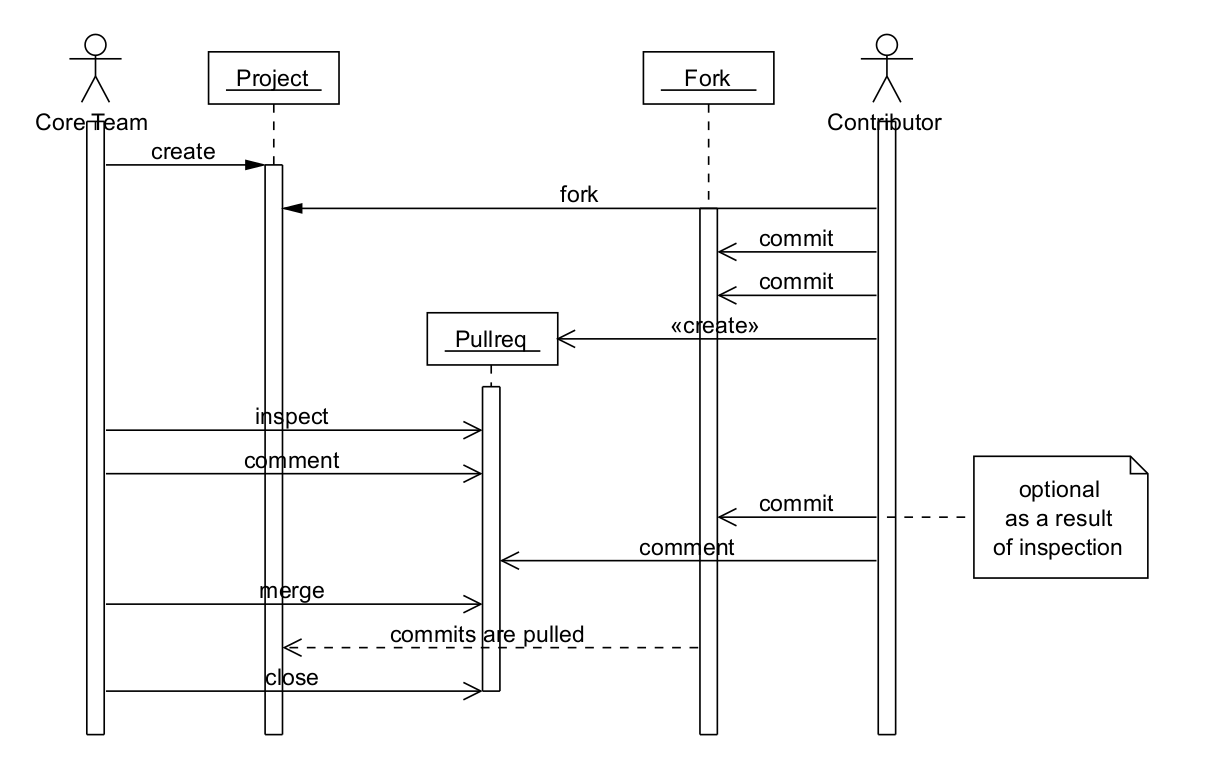
\includegraphics[width=\textwidth]{pull-request-flow}
      \caption{processo do \textit{``pull request''} \cite{gousios2014}}\label{fig:pull-request-flow}
    \end{figure}

    Aquele que deseja contribuir cria para si uma cópia do projeto através de um \textit{fork}. Esta ação cria em seu diretório de trabalho um projeto idêntico ao original, mas ao qual ele tem acesso total de submissão e modificação. Nessa cópia, ele executa as modificações desejadas, geralmente em uma \textit{branch} dedicada para tal \cite{gousios2016}. Ao terminar, ele solicita a integração da \texit{branch} do \textit{fork} de volta ao projeto original. Essa solitação é chamada de \textit{pull-request}, que será analisada por um desenvolvedor com as devidas permissões. Durante esta revisão, o autor pode gerar novas modificações, geralmente atreladas aos pedidos do revisor. Ao final, a mudança é rejeitada (\textit{closed}) ou aceita \textit{merged}.

    Os membros do core também têm suas \textit{branches} revisadas por um processo análogo \cite{6385140,Bosu2014}. A principal diferença é que não há necessidade do \texit{fork}, já que eles tem as permissões necessárias para criar uma nova \textit{branch} no projeto-alvo.

  \section{Desenvolvimento Distribuído de Software}\label{sec:dds}

  O Desenvolvimento Distribuído de Software é uma abordagem em crescente utilização no cenário atual \cite{mens2019}. Este \textit{workflow} descentralizado é caracterizado por membros das equipes de trabalho localizadas em lugares distintos espalhados pelo globo. Modalidades de \textit{home office} e \textit{freelancer} são comuns nestes contextos, mas basta que um membro de uma equipe esteja geograficamente disperso para caracterizar este fenômeno \cite{stadler2019}.  Esta mudança no paradigma tradicional de desenvolviemento colocalizado é patrocinada pelas organizações com o objetivo de reduzir custos, ter acesso a mão de obra mais qualificada e especialmente se manter competitivos num mercado cada vez mais concorrido \cite{herbsleb2001}.

  Assim, os aspectos técnicos do processo produtivo devem se alinhar aos objetivos globais das organizações para dar suporte ao desenvolvimento distribuído e encarar os diversos desafios que permeiam esta mudança. Entre eles, é possível destacar o embate de aspectos socio-culturais, geográficos e de fuso horários. Em suma, estas caracterísitcas inerentes ao desenvolvimento distribuído ameçam a produtividade ao dificultar os processos que envolvem coodernação, comunicação e cooperação \cite{carmel2001}.

\chapter{REFERENCIAL TEÓRICO}\label{chap:trabalhos_relacionados}

Levando em consideração a complexidade e a importância da recomendação de revisores de código, associados com a grande variedade de métodos já propostos para tal fim, foram conduzidas uma revisão e um mapeamento da literatura relacionada <<citar aqui>>. No presente trabalho os principais aspectos e resultados deste estudo serão apresentados, com ênfase naqueles particularmente relevantes aqui. De acordo com parâmetros e diretrizes estabelecidos, \cite{kitchenham2004} o objetivo é apresentar o estado da arte das ferramentas, métodos e potenciais funcionalidades que suportem a escolha de revisores de código. Conhecendo o comportamento histórico do campo, podemos nutrir o desenvolvimento de novas soluções embasadas nas contribuições mais recentes com foco nas lacunas existentes e capazes de contribuir com a evolução das pesquisas relacionadas.

De acordo com estes objetivos, buscamos apresentar em quais contextos a técnica de recomendação automatizada é mais relevante, e quais são as métricas que os pesquisadores utilizam para avaliar e comparar as abordagens propostas. Estas análises podem auxiliar a criar uma estrutura sólida para que novos métodos possam ter sua eficiência avaliada de maneira direta e reprodutível.

Existem tentativas anteriores de reunir e avaliar diferentes métodos de recomendação de revisores, apesar de nenhuma delas envolver um processo sistemático de revisão da literatura relevante. Por isso, não há uma clara classificação dos modelos e os aspectos de reprodutibilidade e replicação dos estudos foram negativamente afetados. Yang et al. \cite{yang2017} apresentam diversos estudos e aplicam um método conhecido numa grande base de dados, tirando conclusões sobre como a eficência dos revisores ativos é muito maior do que aqueles que não participam do processo de forma contundente. Os autores também apresentam uma análise detalhada da base de dados utilizada, possibilitando entender melhor o contexto e a importância do comportamento dos envolvidos nos resultados do processo.

Hannebauer et al. \cite{hannebauer2016} reconhecem que encontrar revisores adequados é um desafio e focam em comparar empiricamente oito diferentes abordagens em quatro conhecidos projetos \textit{open source}. Já Consentino et al. \cite{cosentino2017} apresentam uma revisão sistemática ampla, sobre o processo de desenvolvimento baseado em \textit{pull requests} do GitHub, citando alguns pontos da revisão de código. Apesar de importantes para compreensão da área de pesquisa, as contribuições anteriores não contam com o rigor de uma revisão sistemática da literatura, prejudicando aspectos de reprodutibilidade, adaptabilidade, replicabilidade. Assim, justificamos a necessidade de conduzir uma revisão sistemática para dar suporte teórico à este trabalho, evitando ainda viés por parte dos autores e nutrindo conclusões baseadas em evidências \cite{wohlin2012}.


\section{Revisão sistemática da literatura}\label{sec:revisao_sistematica}

As diretrizes para embasar pesquisas sistemáticas em Ciência da Computação foram propostas por Kitchenham~\cite{kitchenham2004}, ao adaptar abordagens e outras áreas, especialmente das Ciências Méticas. Enquanto o mapeamento traz um panorama geral do desenvolvimento de uma área, a revisão sistemática foca em questões mais específicas e objetivas, muitas vezes relacionadas aos resultados dos estudos. \cite{wohlin2012}. Apesar de geralmente seguir o mesmo protocolo, o escopo, critérios e questões de pesquisa são distintos. Levando em consideração os objetivos deste trabalho a configuração atual da área de pesquisa, ambas as abordagens podem ser úteis. Todas etapas do estudo foram concretizadas por quatro diferentes especialistas, em análises distintas. Todos os critério de inclusão e exclusão dos trabalhos e eventuais divergências foram discutidos em profunidade antes da definição dos resultados.

\subsection{Questões de Pesquisa}

No trabalho conduzido, as seguintes questões foram escolhidas para caracterizar a área de recomendação de revisores de código:;

\subsubsection{\textbf{MQ1: Quem são os principais autores na área?}} Ao identificar os principais autores, embasamos os futuros pesquisadores da área com um ponto de partida para leitura e acompanhamento.

\subsubsection{\textbf{MQ2: Quais são os principais meios de publicação na área?}} O tipo de publicação e conceituação do meio podem ser evidências da maturidade do campo de pesquisa e atenção direcionada pela comunidade acadêmica.

\subsubsection{\textbf{MQ3: Em quais contextos a recomendação de revisores de código é utilizada? (Desenvolvimento global de sofware, indústria, Código Livre)}} O objetivo é endender quais contextos potencializam a necessidade de métodos automatizados de recomendação.

Buscando por um panorama mais espeífico e objetivo, foram propostas as seguintes questões de pesquisa para serem analisadas através da revisão sistemática:

\subsubsection{\textbf{RQ1: Como a eficiência da recomendação dos revisroes é mensurada?}} Para propor novos métodos de recomendação é importante conhecer as métricas de avaliação empregadas nos trabalhos anteriores de forma a fundamentar a comparação dos resultados.

\subsubsection{\textbf{RQ2: Quais informações dos repositórios de software são utilizadas para recomendar os revisores?}} Para propor novos métodos de recomendação é importante entender quais informações foram utilizadas em propostas anteriores, sendo assim possível estendê-las e discutir novas abordagens e aplicações.

Levando em consideração objetivos da abordagem sistemáticas (definidas pelo processo GQM \cite{Basili1984}) e os termos definidos pelo PICOC \cite{Petticrew2008} a \textit{string} de busca foi construída. Termos similares e sinônimos foram incluídos para obter um espectro maior de pulicações. Termos como \textit{``pull-request''} foram adicionados para garantir que trabalhos sobre ``pull-based software development'' (como ilustrado na seção ~\ref{sec:pull_based}) fossem encontrados. Assim, a seguinte \textit{string} foi gerada:

\begin{quote}
  \textit{("software developer" AND developer)  AND  ("reviewer recommendation" OR "commenter recommendation")  AND  (method  OR  tool  OR  solution  OR  framework )  AND  ( "code review" OR "pull-request" OR "pull request" )}
\end{quote}

A \textit{string} de busca proposta foi revisada pelos autores do trabalho anterior separadamente, assim como por um pesquisador externo com o objetivo de validar a sua composição, relevância e emprego e termos correlatos. Buscas \textit{ad-hoc} foram conduzidas para validar o uso dos termos na área e foram encontradas em trabalhos relevantes.


A busca foi executada, com pequenas modificações de sintaxe para aderir aos padrões das diferentes bases de dados. Os resultados foram explorados com o auxílio da ferramenta Parsifal \footnote{http://parsif.al}, muito útil para acompanhar o processo sistemático proposto por Kitchenham~\cite{kitchenham2004}. Na ferramenta foi possível remover trabalhos duplicados, classificar os restantes de acordo com o critério de exclusão e categorizar os restantes de acordo com a relevância para o trabalho. A figura~\ref{fig:workflow} descreve este processo.

\begin{figure}[!htbp]
 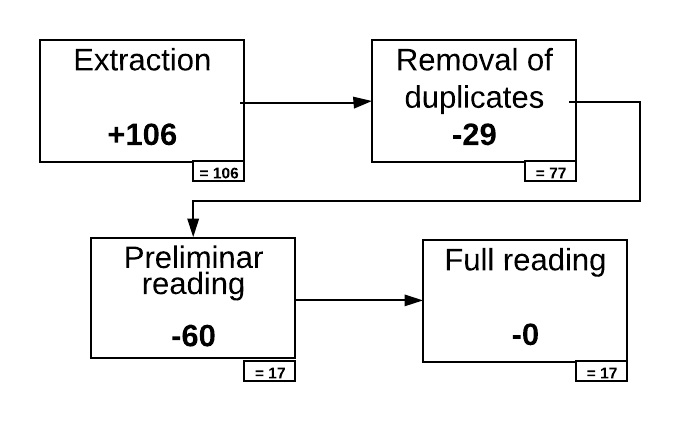
\includegraphics[width=.5\textwidth]{workflow.png}
 \caption{Condução do protocolo sistemático}\label{fig:workflow}
\end{figure}

Ao todo, 106 trabalhos foram encontrados. Destes, 29 foram considerados duplicados, enquanto 60 foram rejeitados de acordo com os critérios de exclusão. A principal razão foi não apresentar um método de recomendação com evidências empíricas de eficiência. Os 17 trabalhos restantes passaram pela leitura completa, constatando-se que todos cumpriam os critérios para inclusão na análise. Respondendo a \textbf{MQ2}, a tabela~\ref{tab:papersperchannel} indica os trabalhos selecionados separados por meio de publicação. o \textit{h5-index} indica o fator de citação da de cada veículo nos últimos 5 anos.


\begin{table}[!htbp]
  \tiny
  \begin{center}
  \caption{Publicações por veículos }
  \label{tab:papersperchannel}
    \begin{tabularx}{\textwidth}{cXc}
    \hline\noalign{\smallskip}
    Reference         & \multicolumn{1}{c}{Channel} & h5-index \\
    \noalign{\smallskip}
    \hline
    \noalign{\smallskip}
    \cite{rahman2016}\cite{balachandran2013}  & ICSE - IEEE/ACM International Conference on Software Engineering & 68                                  \\
    \cite{zanjani2016} & IEEE Transactions on Software Engineering & 52 \\
    \cite{liao2017} & GLOBECOM - IEEE Global Communications Conference & 48 \\
    \cite{costa2016} & SIGSOFT - ACM International Symposium on Foundations of Software Engineering & 43 \\
    \cite{fejzer2017} & Journal of Intelligent Information Systems  & 22 \\
    \cite{jiang2015} & Journal of Computer Science and Technology & 22\\
    \cite{yang2016} &  IEICE Transactions on Information and Systems & 17 \\
    \cite{Thongtanunam2015-1}  & SANER - IEEE International Conference on Software Analysis, Evolution and Reengineering & 13                                 \\
    \cite{yu2014,lee2013} & APSEC Asia-Pacific Software Engineering Conference & 12  \\
    \cite{xia2017} & IEEE/ACM International Workshop on Software Mining & * \\
    \cite{ying2016} &  International Workshop on CrowdSourcing in Software Engineering & *\\
    \cite{yu2014-2}\cite{xia2015}\cite{ouni2016} & ICSME -  IEEE International Conference on Software Maintenance and Evolution  & *\\
    \cite{fu2017} & IWCSN - International Workshop on Complex Systems and Networks & * \\
    \hline
  \end{tabularx}
  \end{center}
\end{table}

Os resultados obtidos através da análise da \textbf{MQ3} servem para direcionar ferramentas de recomendação em contextos onde este tipo de técnica se faz mais relevante. É possível observar que a recomendação de revisores etá relacionada ao desenvolvimento destribuído e ao desenvolvimento ``pull-based''. Esta associação parece ser embasada aos desafios interentes do desenvolvimento global. Ying et al. \cite{ying2016} justificam este fenômeno através do maior número de revisões e revisores, o que dificulta a seleção manual dos envolvidos. Yu et al. \cite{yu2014} mostram que encontrar o melhor revisor para um ``pull request'' é um trabalho tipicamente de ``crowdsourcing''. Assim, para a escolha manual é necessário validar a opinião de muitas pessoas, o que dificulta o processo. Neste contexto também é comum contar com uma riqueza maior de informações graças ao emprego massivo de ferramentas de suporte ao desenvolvimento, onde é a agregação e utilização destes dados ainda é um desafio \cite{rahman2016}.

A maior parte dos trabalhos listados utilizou repositórios de dados \textit{``Open Source''} para testar os métodos propostos, enquanto alguns foram além de utilizaram mecanismos e informações específicas deste tipo de desenvolvimento para criar ferramentas especializadas neste contexto. Devido ao ambiente de rápida interação e grande quantidade de contribuidores esporádicos, as revisões adequadas (muitas vezes movidas pela escolha dos revisores adequados) podem aumentar a retenção de desenvolvedores e influenciar no sucesso do projeto \cite{fu2017}. Neste tipo de processo produtivo é comum existir um grupo seleto de desenvolvedores experientes que agem como guardiões da qualidade, padronização e objetivos dos projetos durante o processo de revisão. Como estes são responsáveis por um conjunto muito grande de revisões \cite{lee2013}, o atraso no assimilação do código proposto à codebase principal pode atrasar as entregas e desencorajar novas contribuições \cite{jiang2015}. Assim, recomendaçoẽs automáticas podem distribuir melhor a carga de revisão e aproveitar melhor as especialidades de cada membro da equipe.

Diante do exposto, os métodos de recomendação deste trabalho levam em consideração aspectos do desenvolvimento distribuído em sua concepção. O desenvolvimento \textit{``Open Source''} é um dos contextos mais maduros e carantes deste tipo de abordagem, e por isso são o principal alvo da ferramenta e campo para avaliação do proposto. Além disso, este tipo de repositório é mais acessível, o que auxilia na realização de experimentos auditáveis e reprodutíveis.




\section{Categorização dos principais trabalhos}\label{sec:metricas_resultados}

Com o objetivo de responder à \textbf{RQ2}, a revisão sistemática separou os trabalhos selecionados em quatro categorias distintas, de acordo com os dados nos quais cada um dos métodos apresentados utiliza.

\subsection{Experiência dos revisores}

Os métodos classificados nesta categoria utilizam a experiência de um revisor como principal informação para recomendá-lo. A lógica é que se ele atuou em revisões parecidas (tanto em região do código quanto em outros aspectos), ele será adequado para a revisão atual.Enquanto Fejzer et al. \cite{fejzer2017} propõem utilizar a similradidade do código submetido com o perfil do revisor, Liao et al. \cite{liao2017} definem um conjunto de tópicos que descrevem a experiência e que pode ser comparado com a necessidade da revisão atual. Thongtanunam et al. \cite{Thongtanunam2015-1} apresenta um abordagem onde o caminho dos arquivos revisados são comparados com o histórico de revisão dos potenciais indicados.

\subsection{Experiência do Desenvolvedor}
Alguns métodos inferem que a experiência do desenvolvedor em contribuições no passado podem indicar na sua capacidade em revisar modificações parecidas. Costa et al. \cite{costa2016} analisam quais foram os responsáveis por mudanças desta região para encontrar candidatos. Rahman et al. \cite{rahman2016} apresentam o CORRECT, um método que analisa a experiência dos desenvolvedores em projetos diferentes mas que contam com tecnologias compartilhadas para recomendar.

\subsection{Redes Sociais}
Uma das abordagens compartilhada entre os métodos mais novos é utilizar os relacionamentos entre desenvolvedores para encontrar os revisores adequados. Ou seja, a partir do histórico de interação (revisão, colaboração, comentários, respostas) é possível inferir quais seriam os melhores revisores para uma nova mudança. Estes relacionamentos são geralmente representados como grafos, construídos com ajuda de análises textuais, proximidade semântica e tópicos das interações passadas. Fu et al. \cite{fu2017} propõe utilzar um grafo baseado nas relações sociais dos desenvolvedores. Xia et al. \cite{xia2017} captura relações implícitas e valoriza interaçoẽs mais recentes. Yu et al. \cite{yu2014,yu2014-2} estende métodos tradicionais em classificação de ocorrências (defeitos, solicitações e etc) para aplicação em recomendação revisores, extraindo informações de discussões e comentários em desenvolvimento global. Yang et al. \cite{yang2016} emprega análise de redes sociais para encontrar revisores baseado na intensidade dos relacionamentos.


\subsection{Abordagens Híbridas}
Alguns métodos reúnem diferentes classes de informação para tentar assimilar as melhores características de cada uma delas. Através da análise de um grafo, Ying et al. \cite{ying2016} consideram tanto a experiência dos desenvolvedores quanto a autoridade no processo de desenvolvimento. Através da ferramenta CoreDevRec, Jiang et al. \cite{jiang2015} utilizam o caminho dos arquivos modificados, a relação pregressa e a atividade dos envolvidos.

Ainda de acordo com a revisão sistemática conduzida, as abordagens baseadas em redes sociais são mais novas e alvo dos trabalhos com mais repercussão na área. Assim, para o escopo deste trabalho foi decidido explorar este tipo de abordagem, que está intimamente relacionado com o desenvolvimento distribuído.



\section{Métricas de avaliação}\label{sec:metricas_revisor}

Respondendo a \textbf{RQ1}, o trabalho de revisão sistemática identifica que a maior parte dos trabalhos utiliza métricas clássicas de sistemas de recomendação para avaliar os métodos, como Top-k \textit{Precision}, \textit{Recall} e \textit{Hit}. Ou seja, é avaliada a proximidade do conjunto de tamanho $k$ que foi recomendado pelo método em relação ao conjunto que um especialista escolheu. Assim, é uma avaliação que compara a capacidade do algoritmo proposto em relação ao que um ser humano especialista faria. a métrica de precisão (\textit{Precision}) mostra o quão parecidos são os conjuntos, enquanto o \textit{recall} aponta quantos items do conjunto do especialista foram ``esquecidos'' pelo método proposto. Já o \textit{hit} indica se pelo menos um membro do conjunto apontado pelo especialista foi considerado pelo algoritmo.

Em contraponto, a revisão sistemática mostrou que alguns autores propõem métodos mais sofisticados para avaliação dos métodos. Esta necessidade se justifica ao considerar que os humanos que indicam revisores não necessariamente são especialistas nesta tarefa. Isso acontece especialmente no desenvolvimento distribuído, onde não é fácil reunir informações sobre todos os envolvidos para embasar estas decisões. Além disso, aspectos de disponibilidade, especialidade, horários e questões culturais deixam ainda mais improvável que os grupos de revisão definidos possam ser considerados como os ideais. Assim, a proximidade do conjunto sugerido com o conjunto efetivamente formado não é suficiente para avaliar os métodos.

Diversas avaliações alternativas são citadas. Yang et al. \cite{yang2016} leva em consideração qual o impacto das recomendações na interatividade das revisões. Outros trabalhos também discutem o impacto positivo dos seus métodos na efiência do processo de revisão \cite{xia2017, liao2017}. A análise focada na eficência e impacto dos métodos de revisão é motivação do presente trabalho, e fomenta aspectos que são detalhados na seção~\ref{sec:avaliacao_review}

\section{Métricas para avaliação do Code Review}\label{sec:avaliacao_review}

Para propor modelos de avaliação voltados para o impacto dos métodos em relação à eficiência do processo de revisão, é necessário estabelecer parâmetros de comparação que embasem tais análises. Além dos aspectos como número de comentários e respostas e tempo de resposta discutidos por Yang et al. \cite{yang2016}. Trabalhos prévios apresentam outras métricas relacionadas à avaliação do processo de revisão, que podem ser aplicadas no contexto da recomendação ao comparar o desempenho de dois grupos distintos de participações em revisões: os sugeridos pelo método e aqueles que não foram. Assim é possível medir se os revisores recomendados tiveram um desempenho melhor durante o processo.

Bosu et al. \cite{bosu2015} conduziram um estudo empírico na Microsoft onde avaliaram manualmente a pertinência de milhares de comentários de revisões. Assim, buscaram descobrir quais características das revisões, revisores e comentários que levaram às interações mais positivas no processo: mais mudanças (frutos de discussões relvantes), adesão aos padrões de desenvolvimento e receptividade por parte dos autores. Já Rahman et al. \cite{rahman2017} analisaM os textos das discussões e encontra correlação da pertinência do revisor com comentários mais úteis. As principais métricas que podem ser objetivamente avaliadas são:

\begin{itemize}
  \item Tempo curto de respostas;
  \item baixo índice de ``stop words'';
  \item interatividade (respostas, comentários, etc);
  \item sentimento positivo;
  \item tamanho dos comentários.
  \item capacidade de gerar mudanças
\end{itemize}

Através de métricas como tempo de resposta e interatividade, é possível avaliar se os revisores indicados potencializam a colaboração e a produção de conhecimento através da discussão, reflexos da revisão de código que devem ser fomentados \cite{Meneely201437, Morales2015171, Bavota201581}. Aspectos como sentimento positivo, baixo índice de ``stop words'' e tamanho dos comentários e a capacidade de gerar mudanças podem indicar que o revisor escolhido foi capaz de interagir positivamente com o processo, gerando valor agregado em soluções melhores e teve perfil e experiências compatíveis para contribuir com código em discussão \cite{bosu2015}.

Tendo como base os resultados da revisão sistemática, da leitura dos trabalhos relacionados, as análises contidas nos capítulos anteriores e o direcionamento aos principais desafios da pesquisa em recomendação de revisores de código, foi possível definir os seguintes tópicos basilares para o trabalho:

\begin{itemize}
  \item O método proposto é direcionado ao contexto de desenvolvimento distribuído, com particularidades para aplicação e avaliação no desenvolvimento \textit{Open Source};
  \item o método proposto utiliza aspectos e análises de redes sociais e relacionamentos entre os desenvolvedores para realizar as recomendações;
  \item o processo de avaliação é pautado na performance dos indicados e de suas interações no processo de revisão.
\end{itemize}

Com estes direcionamentos, o capítulo~\ref{chap:metodos} apresenta a análise exploratória dos datasets escolhidos e embasamento empírico dos métodos propostos.

\chapter{METODOS DE RECOMENDAÇÃO}\label{chap:metodos}

Em convergência com as diretrizes basilares lançadas nos capítulos anteriores, esta seção descreve as análises da colaboração entre desenvolvedores em repositórios ``OpenSource'' que culminaram na proposta de métodos de reomendação para revisão de código. Além da compreensão das características das redes de interação formadas nos repositórios, foram definidos mecanismos para evitar enviesamento dos resultados e excesso de restrição da validade das propostas a determinadas tecnologias ou projetos.

\section{Redes de desenvolvedores}

Interações durante do desenvolvimento de software caracterizam o surgimento de redes sociais de desenvolvedores, denominadas \textit{``social networks''} ou \textit{``developer networks''} \cite{lopez2004}. Observar tais estruturas como grafos é o ponto de partida de diversas aplicações deste tipo de análise, como previsão de defeitos \cite{meneely2008}, triagem de tarefas de manutenção \cite{zhang2012} e encontrar os melhores profissionais para responder determinada dúvida \cite{li2010}. Diversas informações estão disponíveis para a modelagem de tais redes, tanto diretamente das ferramentas de controle versão quanto em ambientes de desenvolvimento mais sofisticados, como o GitHub\footnote{https://github.com} e o GitLab\footnote{https://gitlab.com}. Assim, de acordo com o contexto de cada pesquisa, é possível selecionar quais tipos de interação e seus atributos serão utilizados como vértices, arestas e pesos das representações.

\section{Modelagem da rede}\label{sec:modelagem}
Uma rede social pode ser representada como um conjunto de nós conectados entre si. O objetivo é refletir nesta estrtura a relação entre os indivíduos e a forma que eles interagem. Dentre os dados disponíveis, existem diferentes óticas nas quais os dados podem ser modelados e analisados, de acordo com as conclusões esperadas. No caso deste trabalho, o interesse recai nas interações entre desenvolvedores no processo de \textit{``pull request''} e de revisão de código. Durante esta etapa do desenvolvimento, o revisor interage com o autor comentando em partes específicas do código buscando sanar dúvidas, melhorar a implementação ou evitar que mudanças fora do padrão de codificação sejam admitidas no repositório. A figura~\ref{fig:comment-codereview} representa tal interação.

\begin{figure}[htbp]
 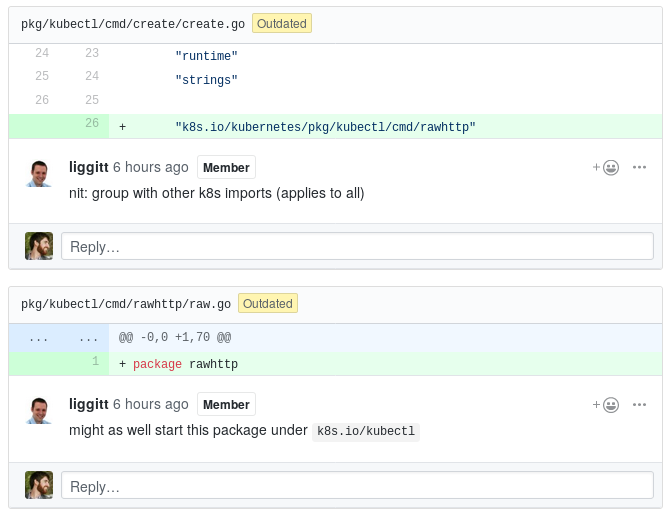
\includegraphics[width=\textwidth]{comment-codereview}
 \caption{Interação entre autor e revisor durante a revisão}\label{fig:comment-codereview}
\end{figure}

Através da API RESTful\footnote{https://developer.github.com/v3/} do GitHub é possível interagir com o repositório e obter estas informações automaticamente, possibilitando a modelagem da rede.

\subsection{Principais características}
No modelo proposto, os desenvolvedores são os nós e as arestas direcionadas entre eles representam os comentários de revisão durante o \textit{``pull request''}. Quando um desenvolvedor cria um comentário em uma revisão, um relacionamento entre ele e o autor é criado ou atualizado. Assim, o modelo é um grafo direcionado $ G = (V, E) $ onde $ V ={v_0, v_1, ... , v_n} $ representa o conjunto de $n$ desenvolvedores e $E$ o conjunto de triplas (arestas) $e_i_j = (v_i, v_j, w)$ entre indivíduos $v_i$ e $v_j$. O peso $w$ é formulado para representar como determinado desenvolvedor influencia outro na perspectiva da revisão. Este valor representa o quão influente é um desenvolvedor sob outros em detrimento do conjunto todo. Ele é calculado considerando cada contribuição $k$ do desenvolvedor $v_i$ para o $v_j$ onde $contrib(v_i,v_j,v_k)$. Valores mais altos de $w$ indicam maior influência de $v_i$ em $v_j$. A figura exemplifica como são representadas as relações entre os desenvolvedores~\ref{fig:relationship}.

\begin{figure}[htbp]
 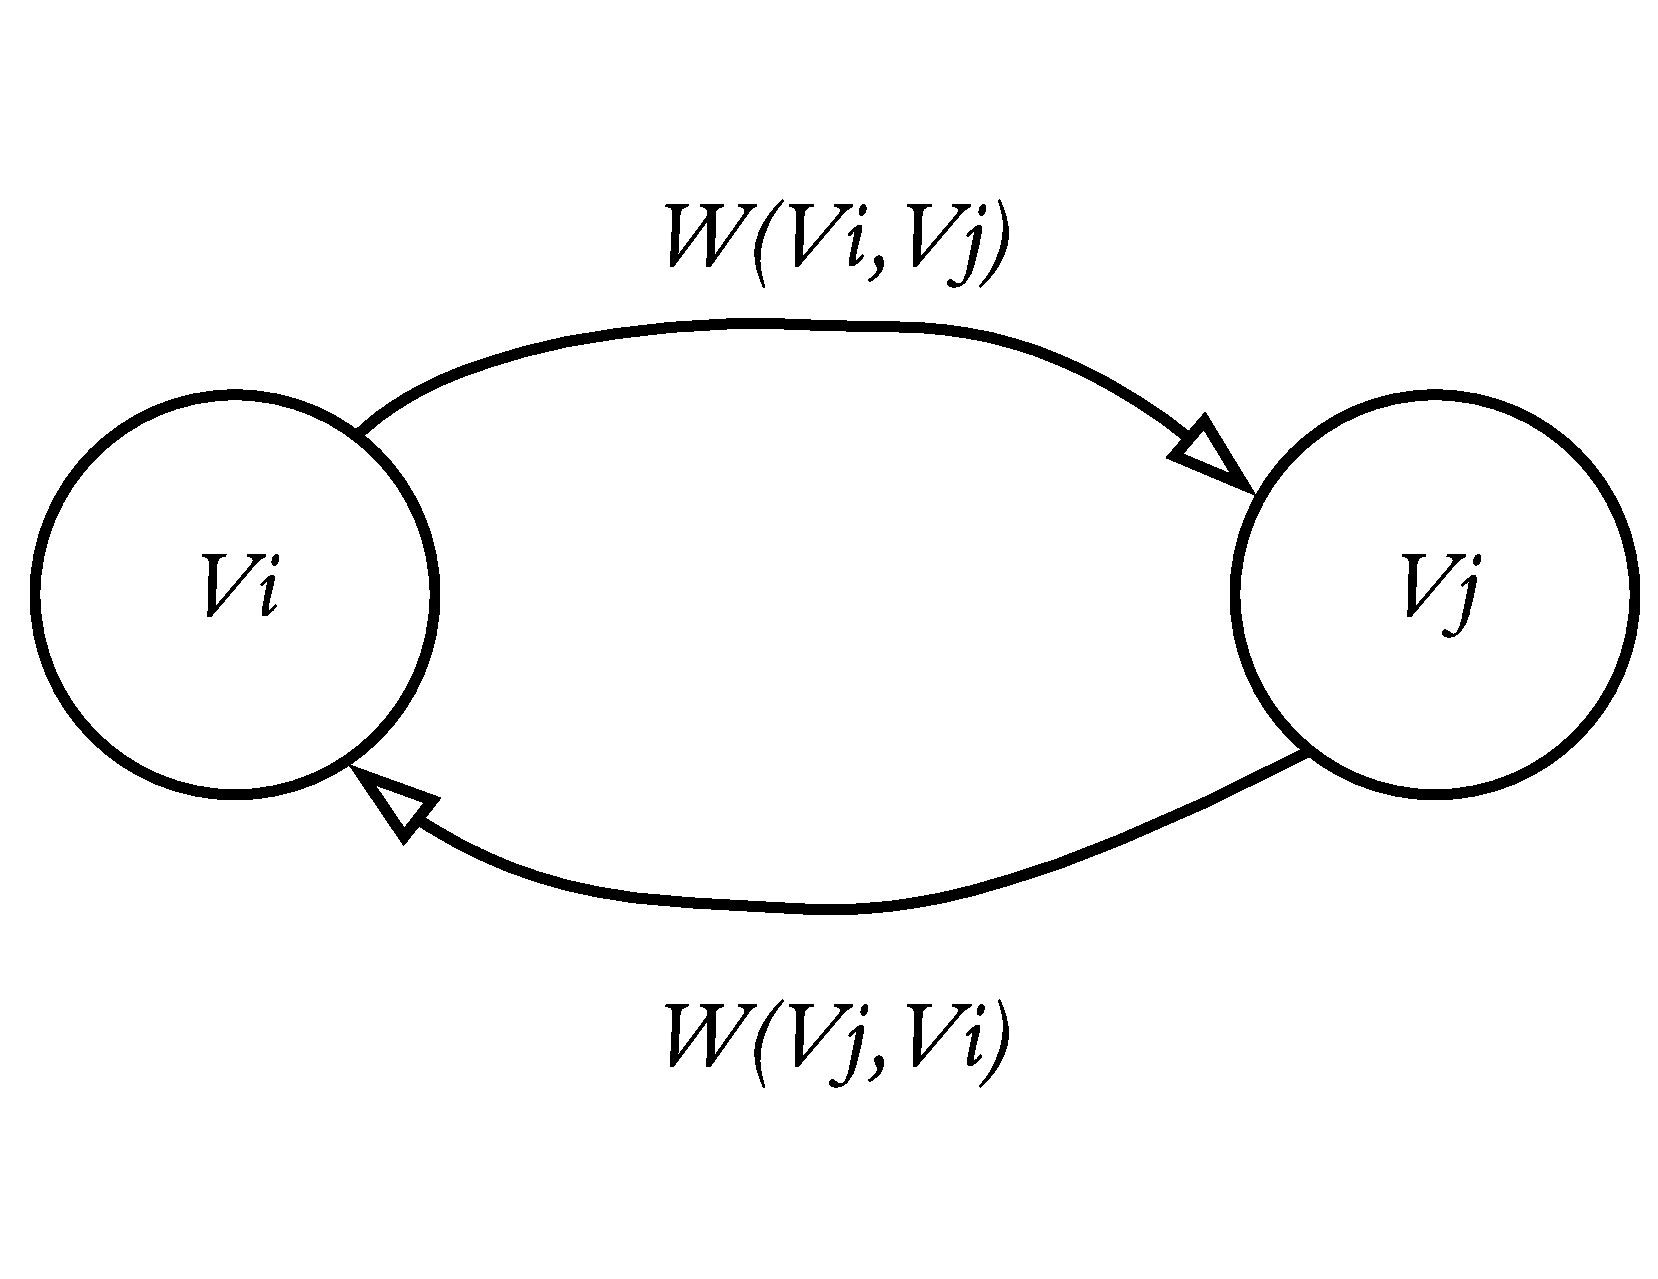
\includegraphics[width=.7\textwidth]{relationship}
 \caption{Representação dos vértices e arestas da rede}\label{fig:relationship}
\end{figure}

Para evitar que interações antigas de desenvolvedores que podem nem estar ativos mais no projeto enviesem as análises, tais ocorrências são penalizadas de modo a valer menos do que interações mais novas. Essa situação é comum em projetos \textit{``Open Source''}~\cite{fogel2005}, além dos casos onde novos desenvolvedores chegam para ocupar as lacunas deixadas neste processo. A figura mostra como esta situação se dá com o tempo, nos gráficos de contribuições (número de \textit{commits}). Enquanto o maior contribuidor (e criador) do Node.js deixa o projeto em 2014, o segundo maior contribuidor chega e continua até os dias de hoje. O \#3 chegou começa seu interação com o projeto mais tarde, enquanto o \#4 foi conteporâneo do idealizador do projeto mas se desligou pouco tempo após sua saída.

\begin{figure}[htbp]
 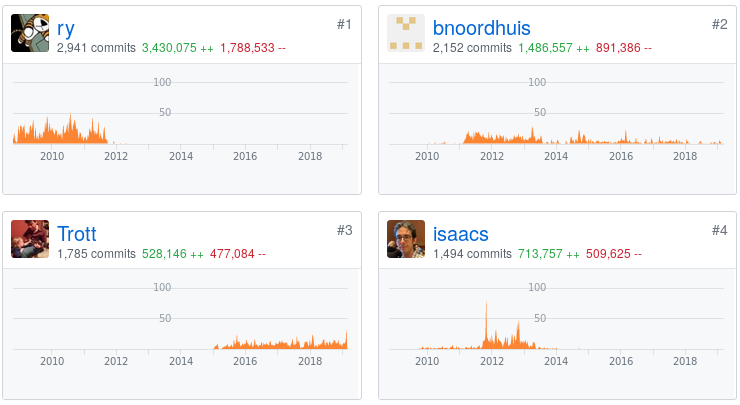
\includegraphics[width=\textwidth]{abandon-nodejs}
 \caption{Troca de participação entre os principais membros do projeto}\label{fig:abandon-nodejs}
\end{figure}

 Assim, o valor de cada comentário $k$ de $v_i$ para $v_j$ decai exponencialmente dquanto mais antigo ele se torna. O valor total $P(v_i,v_j)$ ~\eqref{eq:penalization} é a soma de todas as contribuições de  $v_i$ para $v_j$. A função $inter(v_i,v_j, k)$ retorna cada interação $k$ entre os indivíduos $v_i$ e $v_j$.

Com os valores agregados definidos por $P(v_i,v_j)$, o peso $w_i_j$ é então calculado~\eqref{eq:weight}. $W(v_i,v_j)$ representa qual a participação das interações em direção à $v_j$ vieram de $v_i$. Assim, $w_i_j$ é sempre um número entre $(0,1]$. Quanto mais próximo $w_i_j$ é de 1, maior a influencia de $v_i$ sobre $v_j$. Desta forma, $w_i_j = 1$ significa que $v_i$ é responsável por todas as interações que $v_j$ recebeu.


\begin{equation}
P(v_i,v_j)=\sum\limits_{k=1}^{n}\frac{1}{\exp{days(inter(v_i,v_j, k))}}\label{eq:penalization}
\end{equation}

\begin{equation}
W(v_i,v_j)=\frac{P(v_i,v_j)}{\sum\limits_{k=1}^{n}{P(v_j,v_k)}}\label{eq:weight}
\end{equation}


\section{Análise exploratória da rede proposta}
  Para avaliar a topologia da rede proposta, é necessário instanciar o modelo utilizando dados de projetos de software reais. Assim é possível compreender se as distribuições, cararacterísticas e comportamentos do grafo são compatíveis com o descrito na literatura e se tal contexto permite conclusões relevantes para os objetivos deste trabalho.
  \subsection{Escolha dos repositórios}\label{subsec:escolhaprojetos}
  A escolha dos repositórios influencia na validade das conclusões no contexto estudado e na relevância dos métodos propostos. Por consequência, as seguintes diretrizes foram traçadas para guiar a busca e avaliação dos projetos cujos dados serão território de avaliação e análise desta pesquisa. São elas:

  \begin{enumerate}
    \item O conjunto de repositórios deve ser composto por projetos diversos em tecnologia;
    \item os projetos escolhidos devem ser conhecidos e de popularidade verificável em seus respectivos nichos;
    \item cada projeto deve conter quantidades razoáveis de \textit{``pull requests''} e colaboradores ativos;
    \item os projetos escolhidos devem fornecer regras claras de contribuição, responsabilidade e governança.
    \item os projetos devem estar disponíveis publicamente no GitHub
  \end{enumerate}

  A diretriz 1 auxilia a diminuir o viés a determinada linguagem, propósito, topologia e outros fatores técnicos. A diretriz 2 possibilita a verificação dos resultados com mais naturalidade e leva à potencialização da diretriz 3, que evita que os resultados sejam enviesados para projetos muito pequenos. A diretriz 4 possibilita que diferentes análises possam ser avaliadas de acordo com particularidades do processo de trabalho de cada repositório. Ao seguir a diretriz 4, é possível garantir que os dados serão acessíveis através da interface homogênea disponível para este fim.  Os projetos selecionados constam no top-10 ``projetos mais revisados''\footnote{https://octoverse.github.com/2017/} do GitHub em 2017. A lista é  sumarizada na tabela 4 e apresentada com mais detalhes nas subseções posteriores.

  \begin{table}[htbp]
  \caption{Projetos e principais características}
  \begin{center}
  \begin{tabular}{|c|c|c|c|c|}
  \hline
  \textbf{Projeto} & \textbf{Linguagem Principal} & \textbf{\textit{``Pull requests''}}& \textbf{Estrelas}& \textbf{Contribuidores} \\
  \hline
  Node.js & JavaScript & 18.106 & 62.521 & 2.490 \\
  Kubernetes & Go & 49.946 & 54.849 & 2.186 \\
  Symfony & PHP & 20.002 & 21.088 & 1.891 \\
  Tensorflow & C++ & 11.258 & 130.341 & 2.055 \\
  \hline
  \end{tabular}
  \label{tab:sizemetrics}
  \end{center}
  \end{table}

  \subsubsection{Node.js}

  Node.js\footnote{https://github.com/nodejs} é um framework JavaScript construído sobre o motor V8 do Google Chrome\footnote{https://v8.dev/}. Entre suas principais aplicações está a construção de aplicações ``server-side'' assíncronas e não bloqueantes, voltadas para atender um grande número de clientes simultaneamente. É um projeto ativo no GitHub, sendo o décimo projeto JavaScript com mais estrelas e o 24º global\footnote{https://github.com/search?q=stars\%3A\%3E1\&s=stars\&type=Repositories}. Além disso possui uma estrutura bem definida de governança\footnote{https://github.com/nodejs/node/blob/master/GOVERNANCE.md} que dispõe da tomada de decisões importantes, contribuições da comnunidade e organização de trabalho. Estas características fazem com que as análises das interações de seus participantes possa ser avaliada de acordo com critério objetivos e respaldados pelos responsáveis pelo projeto.

  \subsubsection{Kubernetes}

  Kubernetes\footnote{https://github.com/kubernetes/kubernetes} é um projeto \textit{``Open Source''} escrito em Go voltado para gerenciar softwares em \textit{containers} distribuídos. O projeto provê mecanismos básicos para implantação, manutenção e escalabilidade destas aplicações. Apresenta políticas de segurança bem definidas e documentação das fases do processo de revisão\footnote{https://github.com/kubernetes/community/blob/master/contributors/guide/owners.md} que ajudam a avaliar as hipóteses levantadas durante este trabalho. Contém praticamente 50.000 \textit{``pull requests''}, maior número entre os projetos avaliados. É também o campeão em discussões de toda a plataforma GitHub.

\subsubsection{Symfony}
Symfony\footnote{https://github.com/symfony/symfony/} é um dos mais populares e antigos frameworks PHP, com extensa utilização em aplicações web. Possui políticas claras de contribuição em casos de vulnerabilidades\footnote{https://symfony.com/doc/master/contributing/code/security.html} e é a base de diversos  \textit{Content management system} (CMS) famosos, como o Drupal e o Joomla.

\subsubsection{Tensorflow}

Tensorflow é o projeto mais popular dos analisados neste trabalho, além de ter o maior número de \textit{forks} do GitHub e ser o quinto com mais contribuidores. A tecnologia é desenvolvida em C++ com interface em Python com o objetivo de dar suporte para técnicas de aprendizado de máquina. O processo de revisão é bem documentado e a participação da comunidade são encorajadas diretrizes claras de contribuição, como mostra a figura~\ref{fig:community-profile}.

\begin{figure}[htbp]
 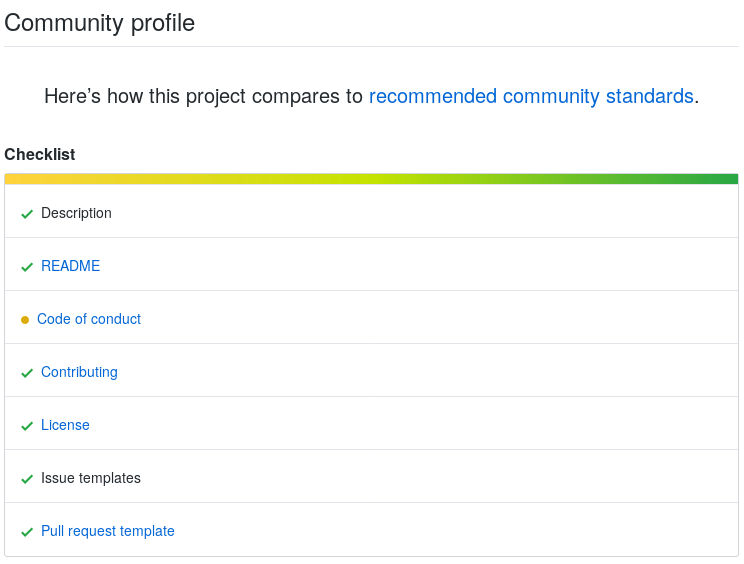
\includegraphics[width=\textwidth]{community-profile}
 \caption{Documentação para dar suporte à contribuição no Tensorflow}\label{fig:community-profile}
\end{figure}



  \subsection{Resultados}

  Os dados foram extraídos através da API do GitHub e carregados em uma instância do Neo4j\footnote{https://neo4j.com/}, um sistema gerenciador de banco de dados orientado a grafos. Para entender como os indivíduos interagem nas redes propostas, algumas análises foram feitas e os principais resultados são detalhados nesta seção.

  Ao calcular a distribuição de grau da rede, é possível entender como os indivíduos partilham a responsabilidade das revisões entre eles. No grafo direcionado, esse valor representa com quantos indivíduos um revisor atuou. Por exemplo no Node.js, como mostra a figura~\ref{fig:outdegree}, é possível observar que um pequeno grupo é responsável pela maior parte das revisões. Este cenário se acentua ainda mais quando a distribuição leva em consideração o peso de cada uma das arestas, como retrata a figura~\ref{fig:outdegree-weighted}. Estas redes são frequentemente classificadas como aleatórias, livres de escala, modulares, entre outras, de acordo com a distribuição do grau~\cite{cross2004}. A distribuição é próxima da lei de potência, o que caracterizaria esta rede como livre de escala.


  \begin{figure}[tbp]
  \centerline{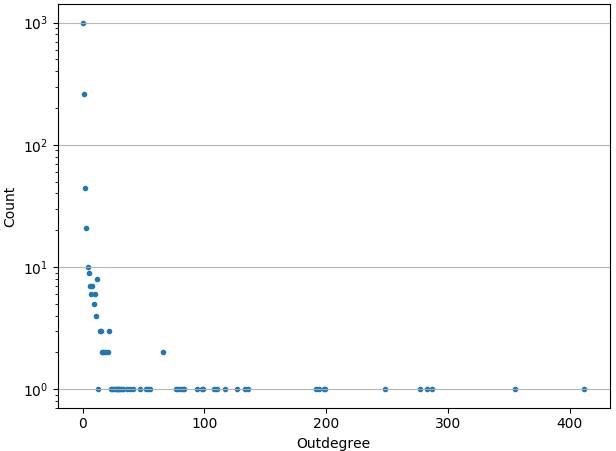
\includegraphics[width=\linewidth]{outdegree}}
  \caption{Distribuição do grau de saída do Node.js}
  \label{fig:outdegree}
  \end{figure}

  \begin{figure}[tbp]
  \centerline{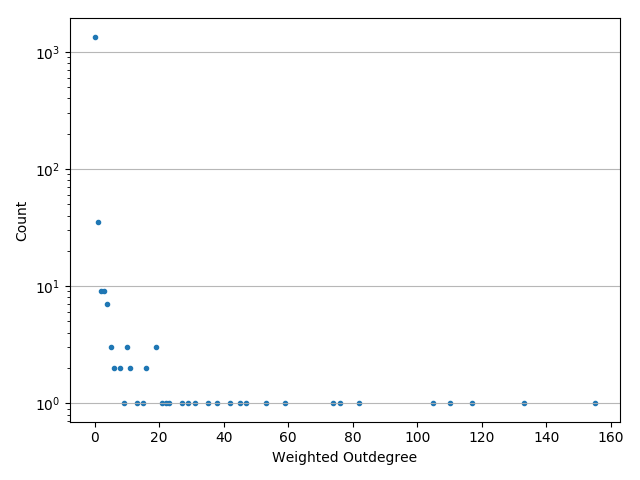
\includegraphics[width=\linewidth]{outdegree-weighted}}
  \caption{Distribuição do grau de saída ponderado do Node.js}
  \label{fig:outdegree-weighted}
  \end{figure}

  Essa tendência acompanha todos os projetos analisados. Apenas 60\% dos usuários revisados no Symfony revisaram outro \textit{``pull request''}, enquanto apenas 4.5\% deles interagiram com mais de 10 outros indivíduos. Os 95\% que menos interagiram são responsáveis por apenas 6\% das interações entre eles. É possível observar essa tendência na figura~\ref{fig:graph-tensorflow}, representação da rede do projeto Tensorflow. O tamanho dos nós é dado pelo seu grau de saída.

  \begin{figure}[tbp]
  \centerline{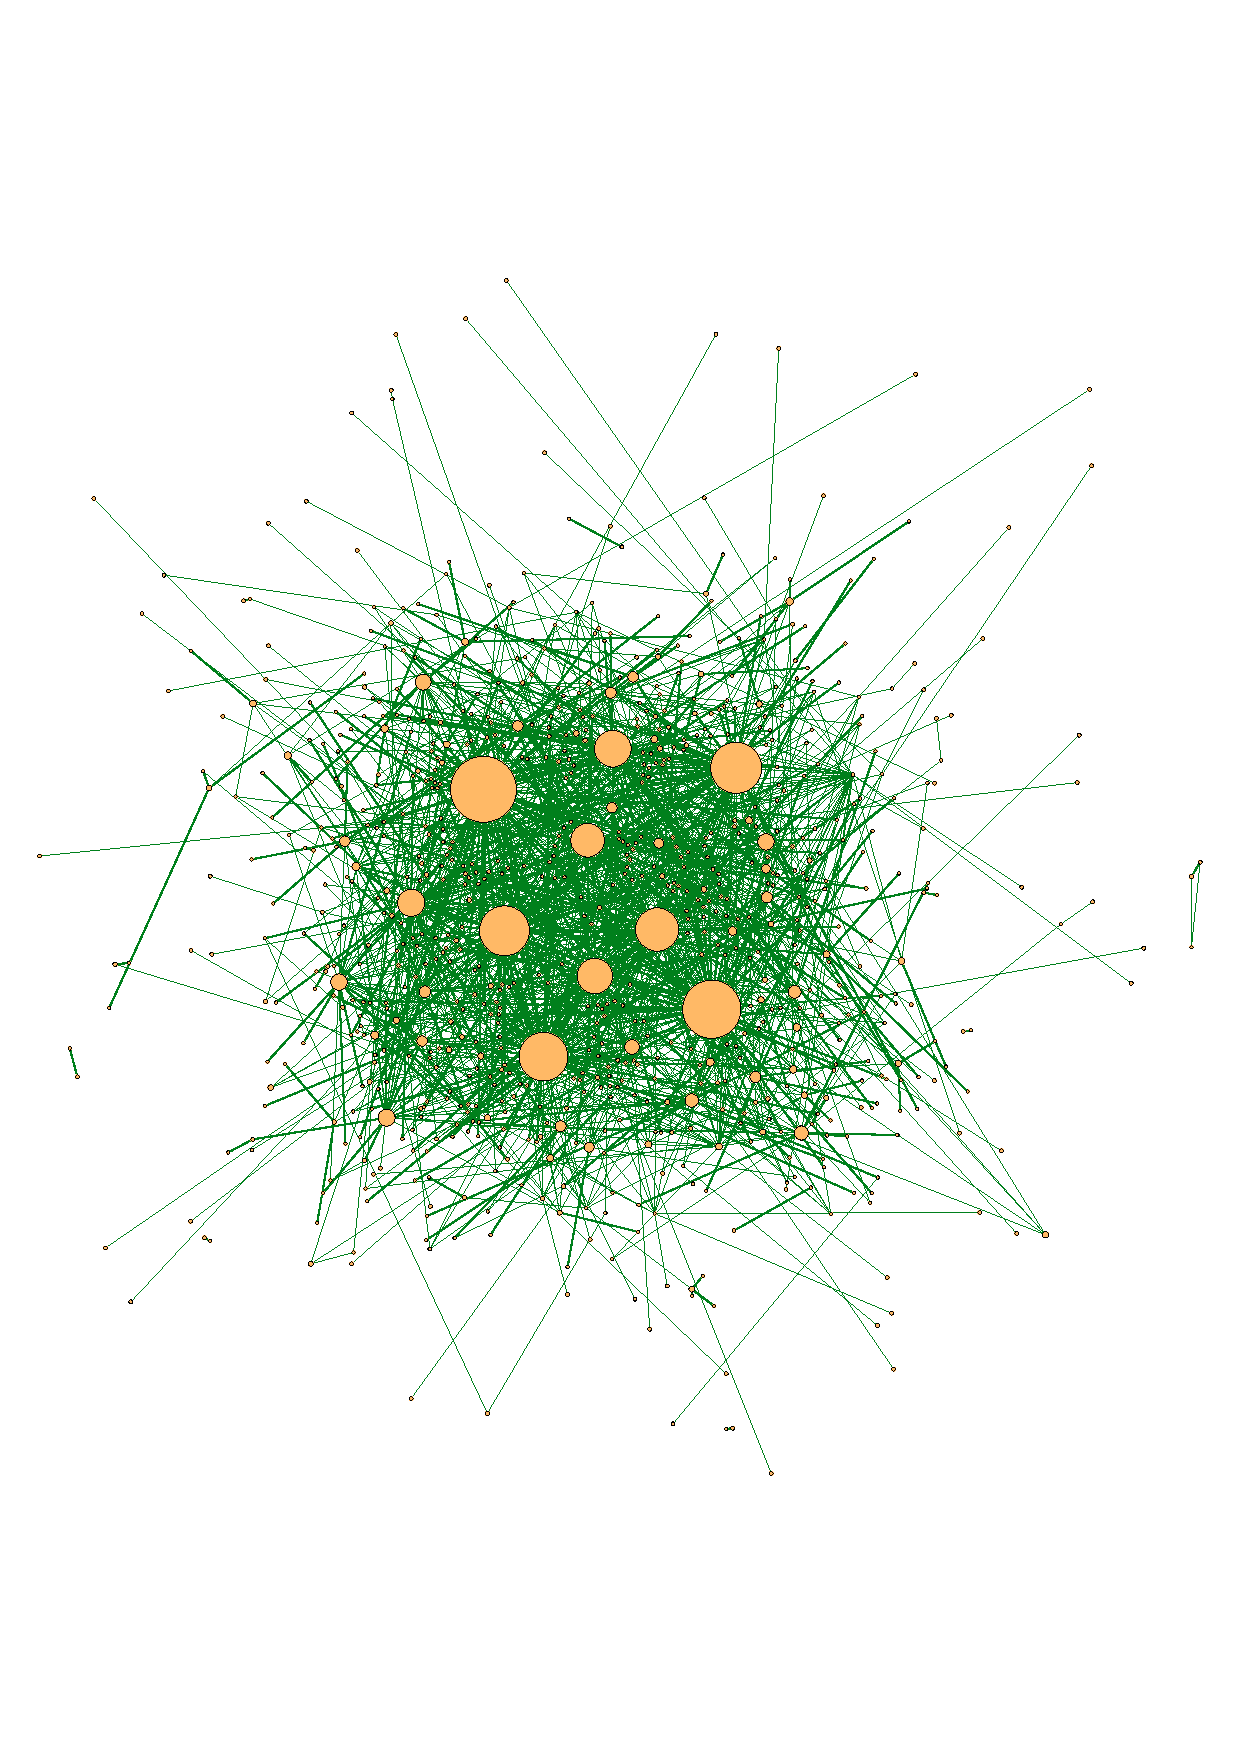
\includegraphics[width=.6\linewidth]{graph-tensorflow}}
  \caption{Representação gráfica da rede do Tensorflow}
  \label{fig:graph-tensorflow}
  \end{figure}


  As distribuições encontradas mostram que poucos indivíduos são responsáveis pela maior parte das interações em revisões dos projetos selecionados. Praticamente toda interação ocorre de alguma forma associada aos principais nós da rede. Por exemplo, no Symfony e no Node.js, existem apenas quatro componentes conexas em toda o grafo. Esta estrutura converge com reportado por trabalhos anteriores \cite{bergquist2001}. Estes especialistas que conduzem a maior parte do processo são podem ser responsáveis pelo projeto como um todo, módulos específicos \cite{firefox2018}, ou tecnologias/atribuições mais específicas \cite{debian2018}. A identificação automatizada da semântica que fundamenta tais distribuições pode levar aos melhores revisores em situações específicas, aumentando a colaboração na revisão. É com esse objetivo que foi aplicada uma abordagem de clusterização nos grafos instanciados, que será detalhada na próxima seção e utilizada como base para alguns dos métodos de recomendação propostos.

  Uma das formas de se compreender a rede é avaliar a distribuição das interações nos \textit{``pull requests''}. Quantos aos comentários de revisão, principal foco deste trabalho, é possível observar que de maneira geral poucos revisores participam do processo. São comentários ligados diretamente ao código e por isso mais técnicos, sendo alvo de um grupo reduzido de indivíduos. A figura~\ref{fig:dist-rc} mostra em formato de histograma a distribuição do número de revisores por \textit{``pull request''}.

  \begin{figure}[htbp]
     \centering
     \begin{subfigure}[b]{0.475\textwidth}
         \centering
         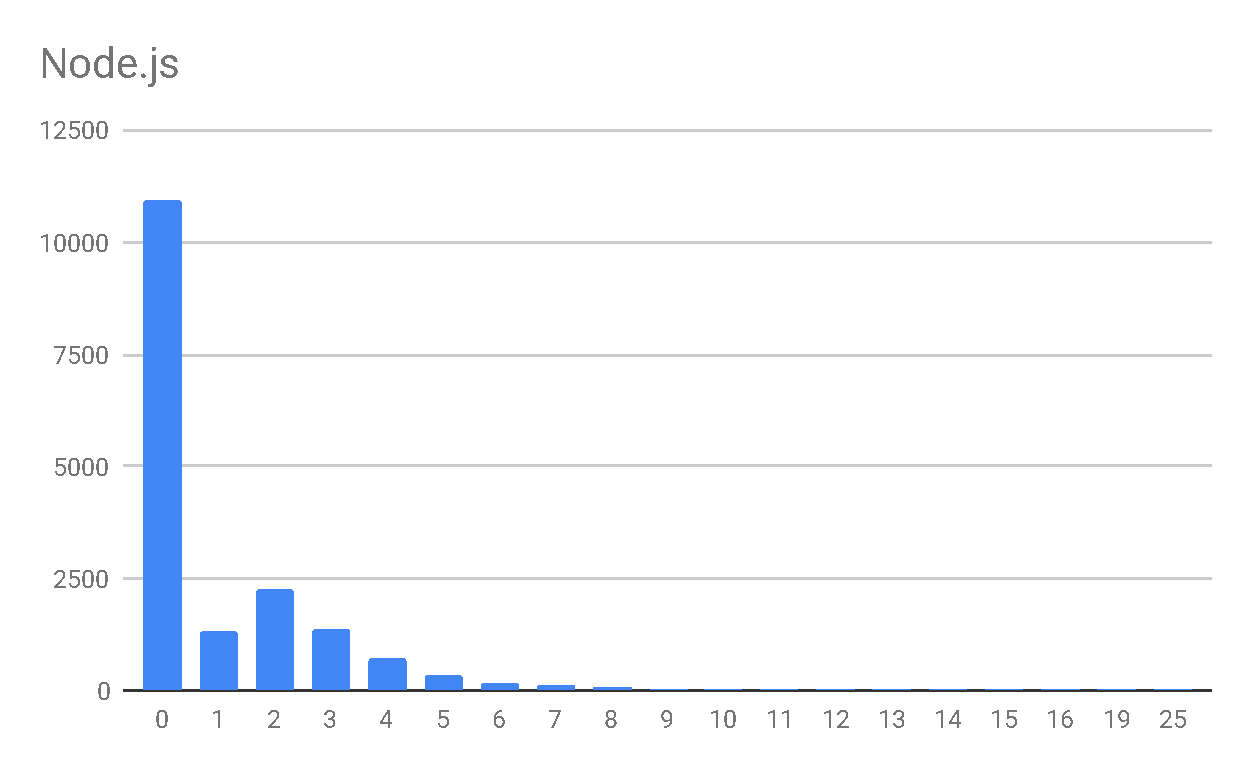
\includegraphics[width=\textwidth]{resultados/dist-rc-node}
         \caption[Node.js]%
         {{\small Node.js}}
         \label{fig:dist-rc-node}
     \end{subfigure}
     \hfill
     \begin{subfigure}[b]{0.475\textwidth}
         \centering
         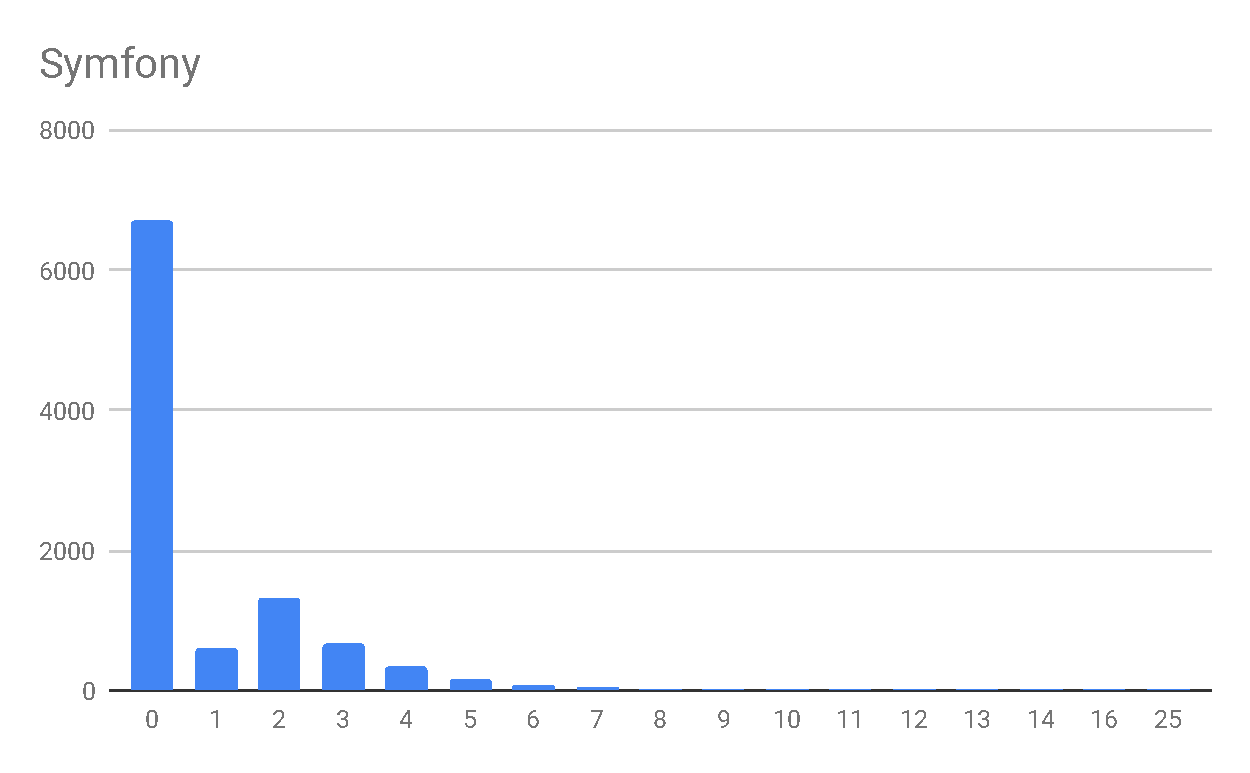
\includegraphics[width=\textwidth]{resultados/dist-rc-symfony}
         \caption[Symfony]%
         {{\small Symfony}}
         \label{fig:dist-rc-symfony}
     \end{subfigure}
     \vskip\baselineskip
     \begin{subfigure}[b]{0.475\textwidth}
         \centering
         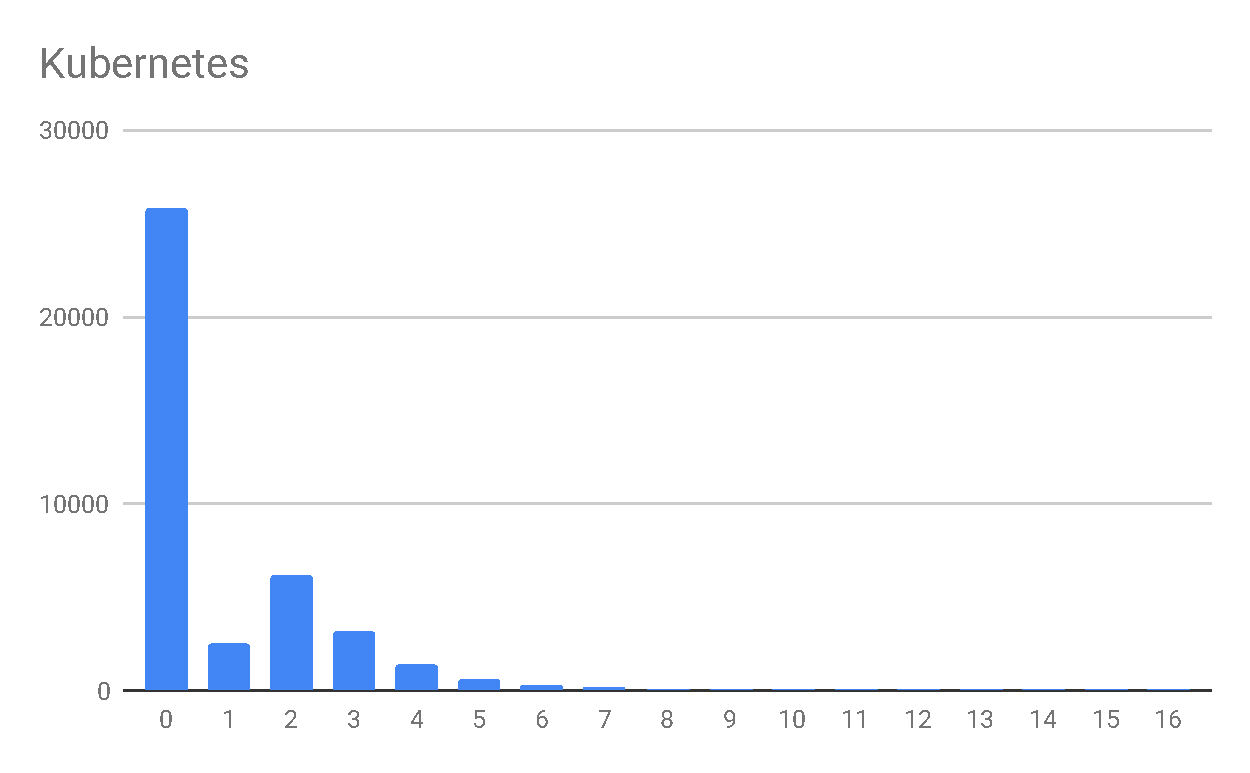
\includegraphics[width=\textwidth]{resultados/dist-rc-kubernetes}

         \caption[Kubernetes]%
         {{\small Kubernetes}}
         \label{fig:dist-rc-kubernetes}
     \end{subfigure}
     \quad
     \begin{subfigure}[b]{0.475\textwidth}
         \centering
         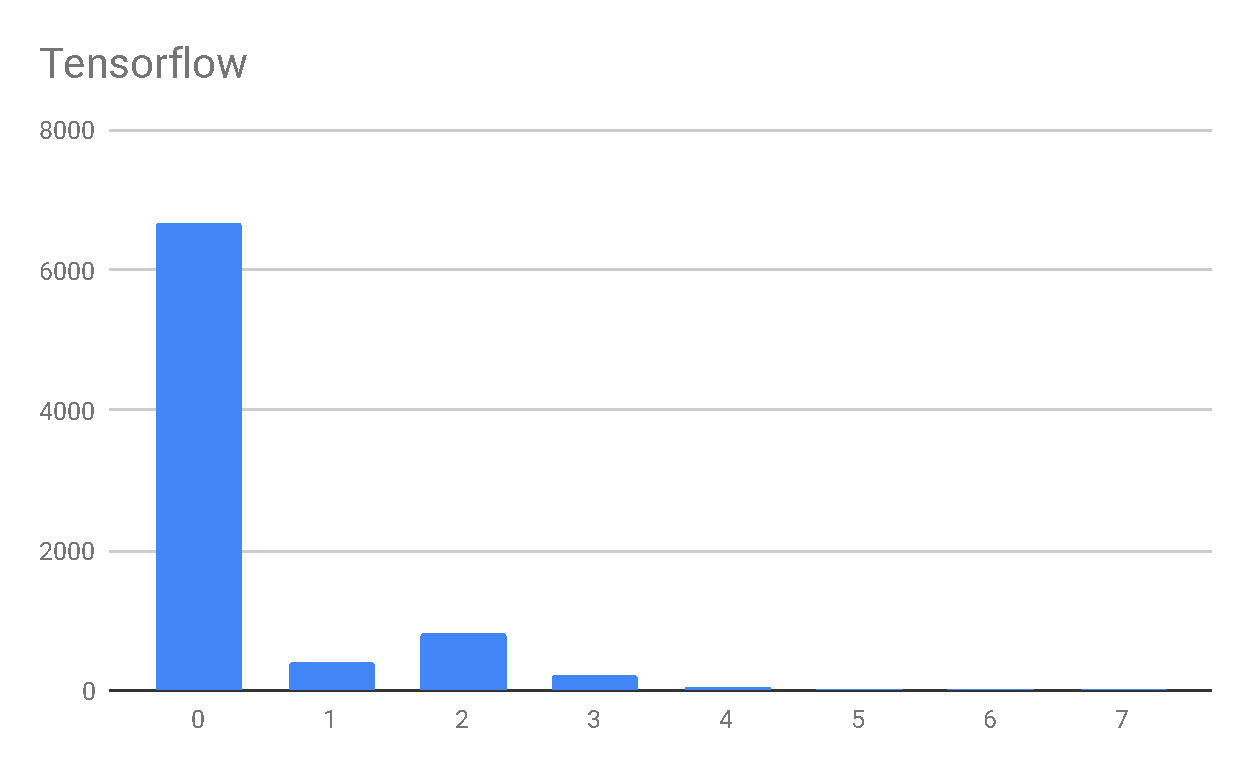
\includegraphics[width=\textwidth]{resultados/dist-rc-tensorflow}
         \caption[Tensorflow]%
         {{\small Tensorflow}}
         \label{fig:dist-rc-tensorflow}
     \end{subfigure}
     \caption[]
     {\small Distribuição de autores de comentários de revisão nos projetos selecionados}
     \label{fig:dist-rc}
 \end{figure}

  É possível observar em todos os projetos que a maior parte dos casos menos de três revisores participam do processo. Existem muitos casos onde não há nenhum tipo de interação de revisão, possivelmente em \textit{``pull requests''} menores ou mais simples. Este comportamento se mostra menos acentuado em alguns projetos quanto o assunto são comentários gerais, de discussões que não necessariamente são técnicas durante o processo. É o que demonstra a figura~\ref{fig:dist-dc}, análoga às anteriores mas contando o número de autores de comentários de discussão nos \textit{``pull requests''}.

  \begin{figure}[htbp]
     \centering
     \begin{subfigure}[b]{\textwidth}
         \centering
         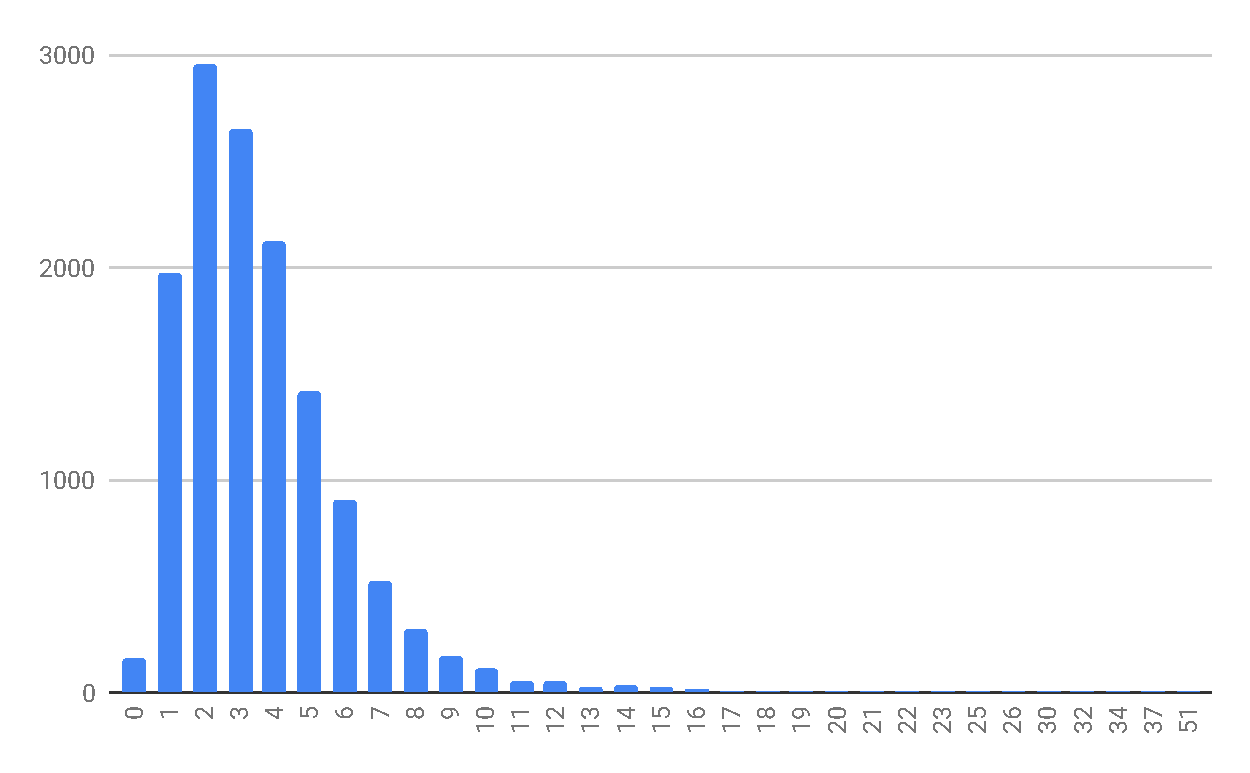
\includegraphics[width=\textwidth]{resultados/dist-dc-node}
         \caption[Node.js]%
         {{\small Node.js}}
         \label{fig:dist-dc-node}
     \end{subfigure}
     \vskip
     \centering
     \begin{subfigure}[b]{\textwidth}
         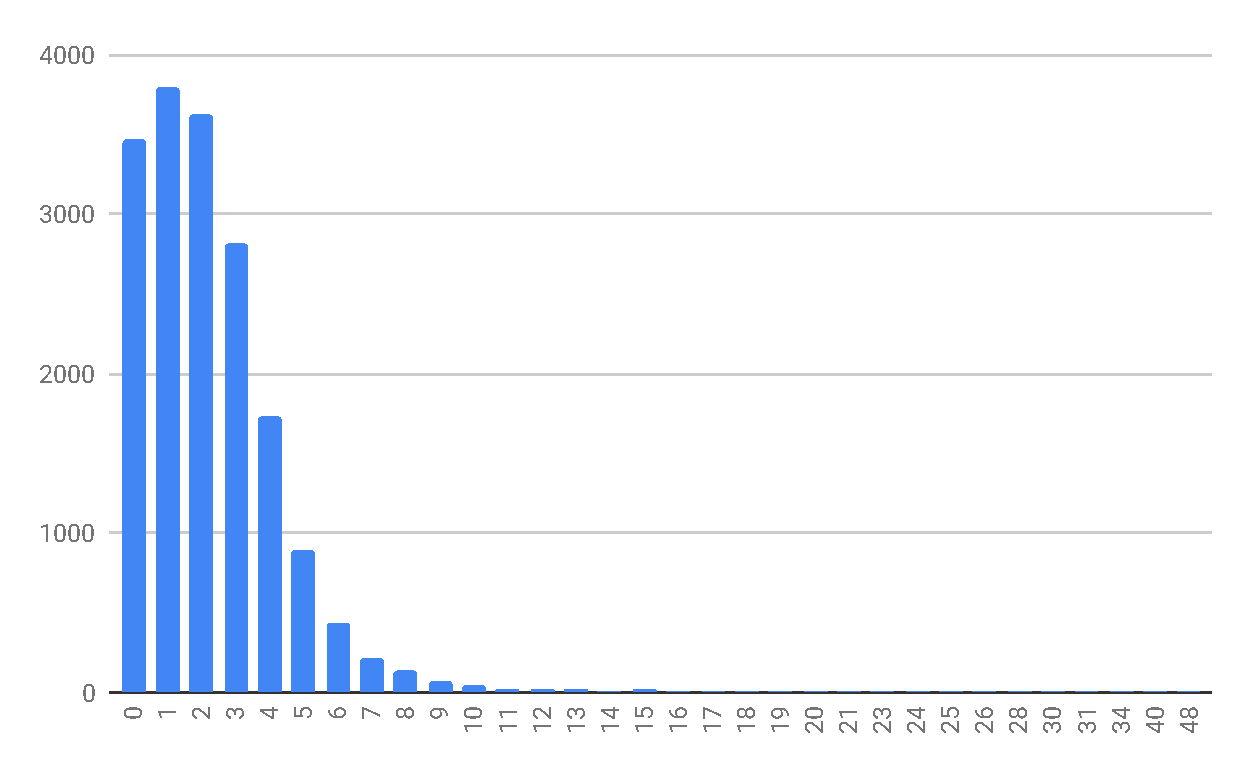
\includegraphics[width=\textwidth]{resultados/dist-dc-symfony}
         \caption[Kubernetes]%
         {{\small Kubernetes}}
         \label{fig:dist-dc-symfony}
     \end{subfigure}
     {\small Distribuição autores de comentários de discussão em dois dos projetos selecionados}
 \end{figure}
 \label{fig:dist-dc}

\section{Clusterização}

  Uma das formas de entender melhor a estrutura de uma rede social é através de métodos de clusterização.  Neste caso a proximidade dos indivíduos é calculada pelas suas interações, com um método de agrupamento \cite{meng2014}. No perfil de projetos-alvo deste estudo é importante que o método escolhido leve em considerações duas particularidades pertinentes:

  \begin{enumerate}
    \item É preciso que os indivíduos possam se enquadrar em mais de um grupo;
    \item o número de grupos (ou \textit{clusters}) deve ser inferido automaticamente.
  \end{enumerate}

  Estas exigências se dão devido a natureza da organização e forma de trabalho dos projetos \textit{open source}. Especialmente os experts acabam por participar de diversas frentes de trabalho, devido à mão de obra reduzida. Além disso, a quantidade de grupos pode variar drásticamente de um projeto para outro, inclusve dentro do mesmo projeto mas em momentos diferentes do ciclo de vida de desenvolvimento. A próxima seção detalha o algorimo escolhido e como ele trata as questões levantadas.

  \subsection{NetSCAN}\label{subsec:netscan}

  NetSCAN~\cite{horta2018} é um algoritmo de clusterização baseado em densidade, que estende o conhecido DBSCAN \cite{ester1996}. As principais diferenças são que o NetSCAN considera o direcionamento das arestas e a possibilidade de um indivíduo participar de mais de um grupo. Como é esperado encontrar grupos tênues, informais e com divisões de responsabilidades sutis, NetSCAN atende os objetivos. Os indíviduos \textit{core} de cada cluster são identificados, podendo estes também estarem sobrepostos em outros silos.



  NetSCAN espera dois parâmetros, \textit{eps} e \textit{minPts}. O primeiro indica o peso mínimo de uma aresta para ser considerada no processo de agrupamento, enquanto a segunda é o \textit{threshold} que indica a pontuação para um indivíduo ser considerado como \textit{core}. O primeiro permite evitar que nós de baixa relevância influenciem na formação dos grupos, enquanto o segundo permite que apenas indivíduos de alta participação sejam considerados como peças centrais dos silos.

  Para proporcionar a melhor escolha de parâmetros, foram testadas diferentes combinações em busca de otimizar a silhueta dos grupos~\cite{tan2005}. Essta métrica usa a distância entre os nós contidos em um \textit{cluster} para comparar a similaridade entre eles. A ideia é que a proximidade deles seja maior que em relação a membros externos dos grupos. O índice varia entre -1 e 1 onde valores mais altos indicam grupos mais coesos.~\cite{almeida2011}. Na figura~\ref{fig:silhouette_boxplot} é possível ver a distribuições de silhuetas na clusterização otimizada do Node.js. O número de \textit{clusters} é inferido automaticamente pelo NetSCAN tendo como referência as características da rede.

  \begin{figure}[tbp]
  \centerline{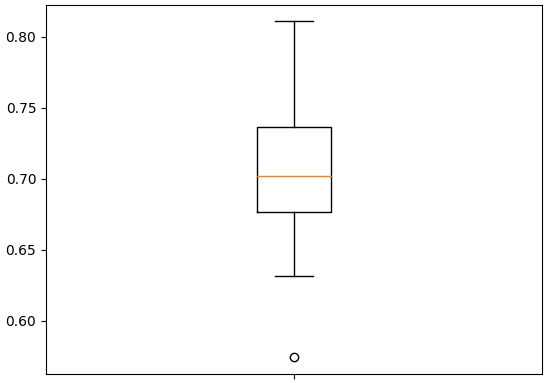
\includegraphics[width=.8\linewidth]{silhouette_boxplot}}
  \caption{Silhuetas do Node.js}
  \label{fig:silhouette_boxplot}
  \end{figure}

  A processo de otimização foi conduzido para todas os projetos, como apresenta a tabela~\ref{tab:netscan_optimize}. Estes são os valores utilizados todas as análises descritas posteriormente neste trabalho.
  \begin{table}[htbp]
  \caption{Valores otimizados pela silhueta de cada projeto}
  \begin{center}
  \begin{tabular}{|c|c|c|}
  \hline
  \textbf{Projeto} & \textbf{\textit{eps}} & \textbf{\textit{minPts}} \\
  \hline
    Node.js    & 0.45 & 10     \\
    Kubernetes & 0.45 & 12     \\
    Symfony    & 0.38 & 14     \\
    Tensorflow & 0.3  & 10    \\
  \hline
  \end{tabular}
  \label{tab:netscan_optimize}
  \end{center}
  \end{table}

  NetSCAN é encapsulado em um plugin para o Neo4j\footnote{https://github.com/vitorhorta/netscan-neo4j}, e pode ser executado diretamente através do Cypher com parâmetros dinamicamente definidos. Este processo é detalhado na seção seguinte.

  \subsection{Execução}

  A execução dos métodos de clusterização é contida, junto com outras funcionalidades, na ferramenta cuja arquitetura é detalhada na seção~\ref{chap:solucao}. Os dados são automaticamente carregados para uma instância Neo4j e o algoritmo aje com os parâmetros debatidos nas seções anteriores. A figura~\ref{fig:cluster} ilustra um dos \textit{clusters} encontrados.

  \begin{figure}[tbp]
  \centerline{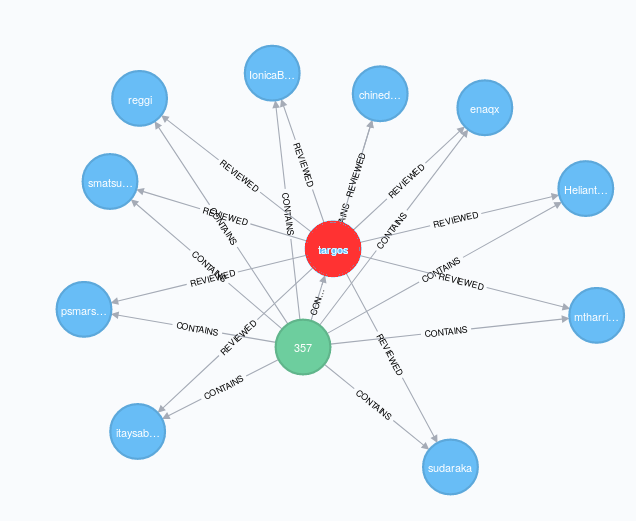
\includegraphics[width=\linewidth]{cluster}}
  \caption{Representação de um dos \textit{clusters} do Kubernetes}
  \label{fig:cluster}
  \end{figure}

  O os nós em azul são os participantes do \textit{cluster}, todos tiveram uma contribuição revisada pelo indivíduo \textit{core} representado em vermelho. A entidade caracterizada em verde é o \textit{cluster} em si, que pode ser utilizado para identificar os seus participantes através da relação do tipo \textit{CONTAINS}.

  Idealmente, os grupos encontrados devem corresponder à grupos reais de trabalho dentro de um projeto. Ou seja, deve existir uma corroboração semântica do que foi encontrado: equipes que frequentemente trabalham em conjunto, grupos focais em tecnologias ou áreas específicas, times que se destacam em módulos ou funcionalidades, entre outras divisões. A próxima seção propõe métodos objetivos para avaliar tais caracetísticas que podem indicar maior efetividade da clusterização como base para algoritmos de detcção de especialistas e recomendação para revisão.

  \subsection{Avaliação da clusterização}

  Duas formas de avaliação semântica foram aplicadas neste trabalho. A primeira diz respeito à pertinência dos \textit{cores} encontrados enquanto desenvolvedores influentes e responsáveis pelo projeto. A segunda verifica a diferença entre as atividades e os principais focos dos grupos destacados.

  Na primeira abordagem, podemos utilizar duas informações dos repositórios como base: as reações positivas e negativas que os comentários dos \textit{cores} geram e se eles são oficialmente listados como responsáveis/membros do projeto, com poder formal sobre as decisões e revisões.

  É possível verificar que os \textit{cores} são alvos da maior parte das reações durante o processo. Esta proporção no Symfony é visualizada em escala logarítmica na figura~\ref{fig:chart-reactions-symfony}.  Enquanto as maiores diferenças em relação aos indivíduos comuns é observada nas reações positivas como ``+1'' (conhecida também como \textit{``thumbs up''}), a diferença é pequena para expressão de sentimentos negativos. Esse é um comportamento que se repete em todos os projetos. No node.js, 81\% dos \textit{cores} indicados estão presentes no conjunto que recebeu mais reações positivas. A lista tem 27 elementos, o mesmo número de \textit{cores} encontrados. No Symfony esse valor é de 75\%, enquanto no Kubernetes chega a 78\%.


  \begin{figure}[htbp]
    \centerline{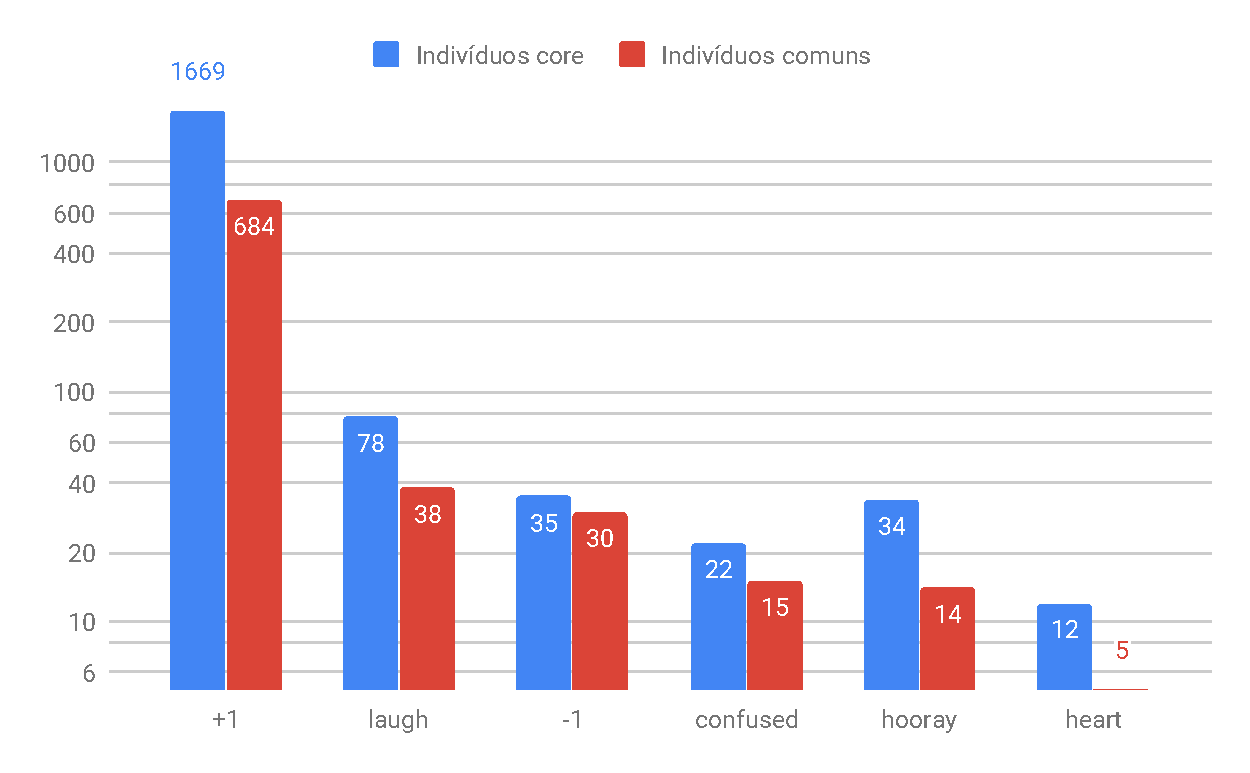
\includegraphics[width=\linewidth]{chart-reactions-symfony}}
    \caption{Comparação das reactions recebidas por usuários \textit{cores} e comuns no Symfony}
    \label{fig:chart-reactions-symfony}
  \end{figure}


  Quanto à responsabilidade dos desenvolvedores \textit{core} no projeto, é possível analisar se eles possuem permissões de aprovar \textit{``pull requests''} e de outras tarefas administrativas no projeto. A tabela~\ref{tab:prop-core-users} mostra os resultados da proporção de \textit{cores} detectados que efetivamente são dotados desse nível de permissão. É possível que participantes não possuem tal concessão hoje já tenham tido em um passado recente, mas a informação histórica não está disponível para consulta.

  \begin{table}[htbp]
  \caption{Proporções de \textit{cores} detectados com direitos administrativos}
  \begin{center}
  \begin{tabular}{|c|c|}
  \hline
  \textbf{Projeto} & \textbf{Proporção} \\
  \hline
  Node.js    & 78\%      \\
  Kubernetes & 77\%      \\
  Symfony    & 69\%      \\
  Tensorflow & 69\%      \\ \hline
  \end{tabular}
  \label{tab:prop-core-users}
  \end{center}
  \end{table}

Observar distinções entre os grupos do ponto de vista da natureza das tarefas executadas é uma das formas de analisar se os silos detectados são de fato pertinentes no mundo real. No caso dos projetos analisados, as categorias nas quais os \textit{``pull requests''} foram enquadrados formam uma indicação para tal avaliação. No GitHub essas categorias são dadas como forma de \textit{Tags} ou \textit{Labels}, que são associadas aos \textit{``pull requests''} no momento de sua criação, como exemplifica a figura~\ref{fig:labels}.


  \begin{figure}[htbp]
    \centerline{\fbox{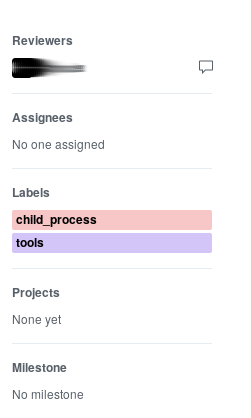
\includegraphics[width=.3\linewidth]{labels}}}
    \caption{\textit{Labels} associadas a um \textit{``pull request''} no Node.js}
    \label{fig:labels}
  \end{figure}

Para avaliar tal distinção, foram comparados quais \textit{clusters} trabalham com quais \textit{Labels}. Foram selecionadas as 20 \textit{Labels} mais utilizadas de cada projeto e quais clusters trabalham com tais categorias entre suas 20 mais utilizadas. O resultado pode ser representado como u grafo na figura~\ref{fig:graph-labels-kubernetes}. Em todos os projetos analisados, foi possível observar a tendência de determinados tópicos de trabalho serem conduzidos principalmente por um conjunto reduzido de grupos.

\begin{figure}[htbp]
  \centerline{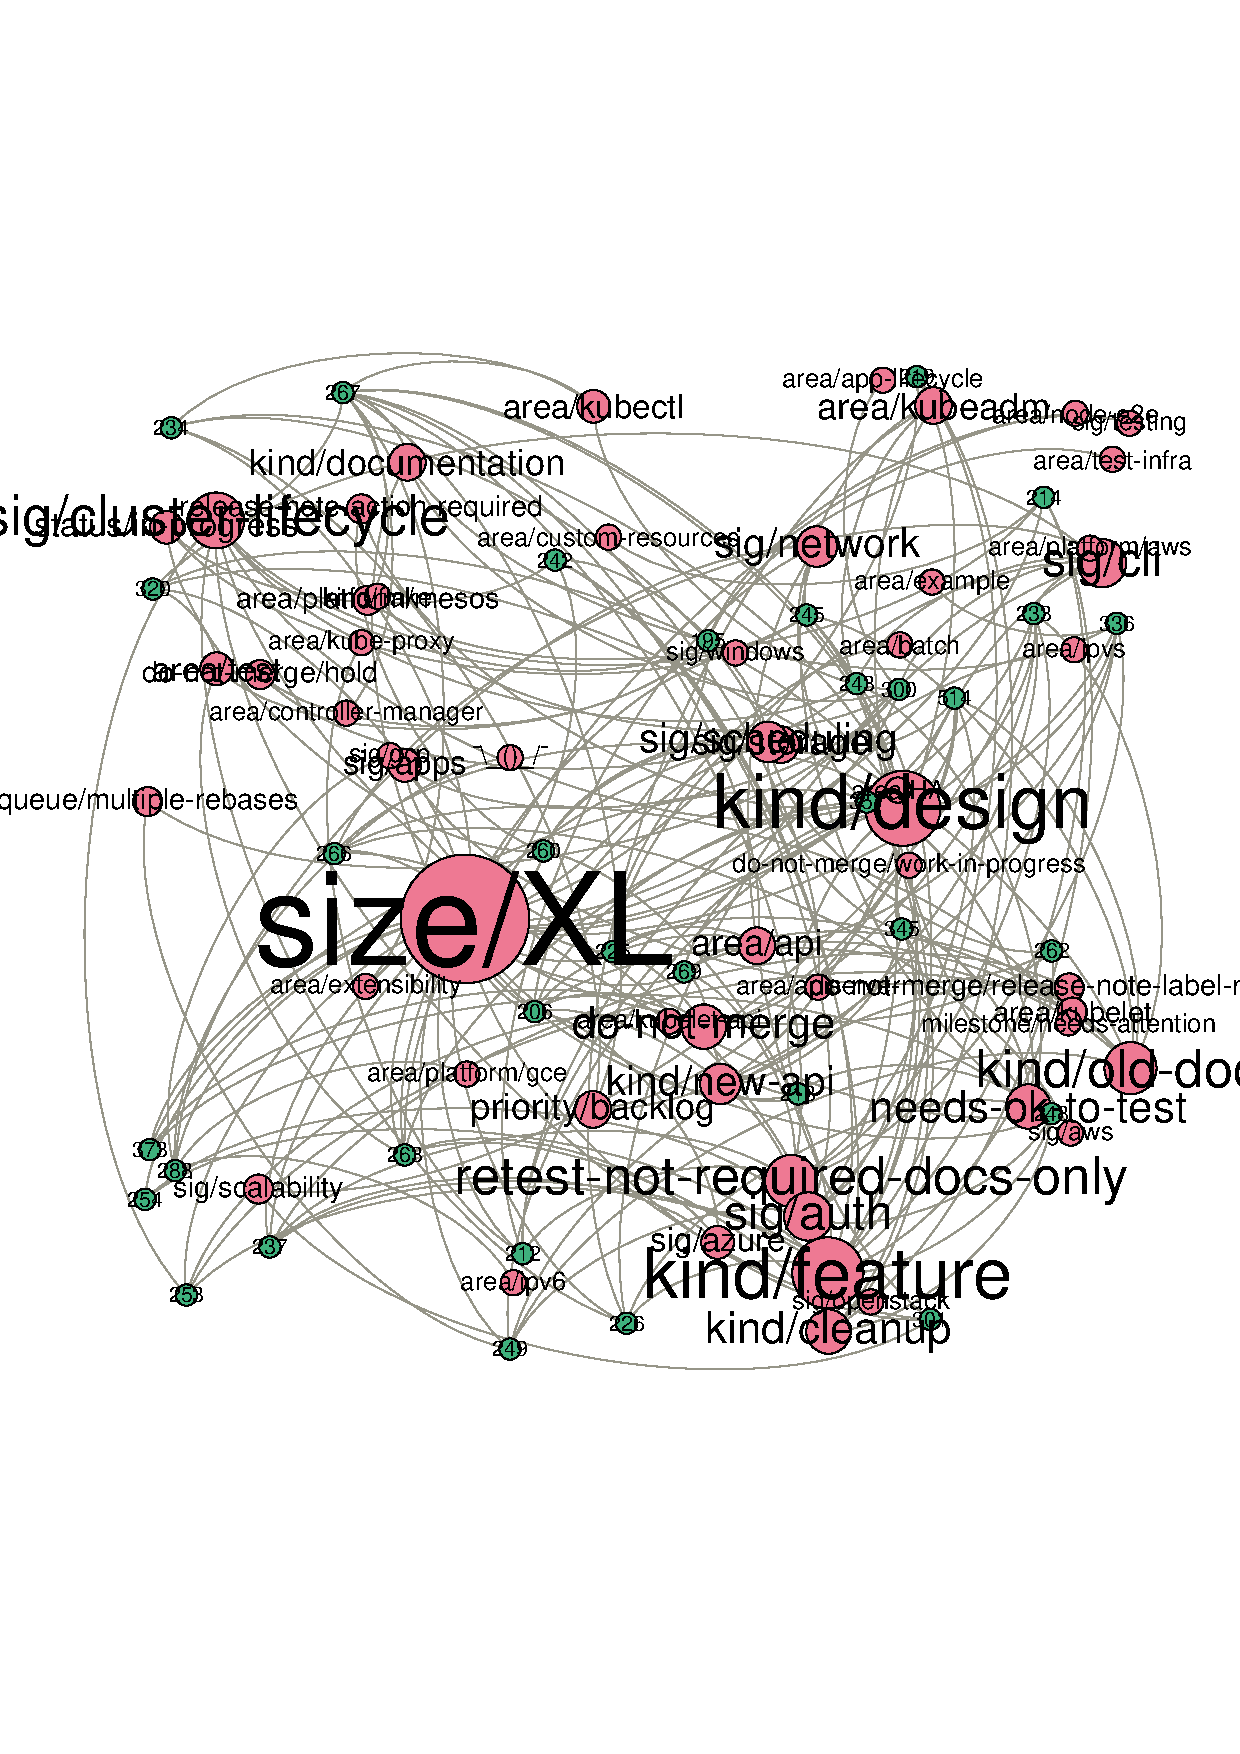
\includegraphics[width=.7\linewidth]{graph-labels-kubernetes}}
  \caption{\textit{Clusters} associados a cada \textit{``Label''} no Kubernetes}
  \label{fig:graph-labels-kubernetes}
\end{figure}

No grafo da figura \ref{fig:graph-labels-kubernetes}, os grupos são representados na cor verde e as \textit{Labels} em rosa. O tamanho da representação de cada \textit{Label} se dá pelo seu grau de entrada. Assim, as categorias maiores estão associadas à mais grupos. É o caso das categorias que representam aspectos de documentação, processo de trabalho e testes, como o caso de \textit{``kind/feature''} e \textit{``kind/design''}, que são divisões mais genéricas. Já as tarefas de àreas específicas, como \textit{``area/kubectl''} e \textit{``area/api''} são conduzidas por menos grupos, mostrando uma especialização das atribuições.

As avaliações conduzidas apontam que os grupos e \textit{cores} encontrados podem ser reflexos das divisões de trabalho, influência e responsabilidade dentro dos projetos selecionados. Tal asserção fundamenta a utilização da rede modelada e da técnica de clusterização escolhida nos métodos de recomendação de revisores escolhidas, uma vez que a capacidade técnica e experiência dos especialistas pode aumentar a colaboração durante o processo~\cite{Bosu2014, kovalenko2018}.


\section{Métodos de recomendação}
  Os métodos propostos utilizam características observadas na rede modelada e nos \textit{clusters} detectados para recomendar revisores que possam potencializar a colaboração durante o processo de revisão de código, de acordo com os objetivos definidos deste trabalho. A proposição de três métodos distintos e complementares se fundamenta em aproveitar as diferentes particularidades dentro do contexto de pequisa para que os utilizadores das abordagens possam escolher os resultados que mais se encaixem com os objetivos da organização. Todos os métodos recebem apenas um parâmetro $k$, que representa quantas recomendações deverão ser executadas.

  \subsection{RandomCore}
    Este método emprega os \textit{cores} encontrados durante a clusterização como referências não só dos grupos de trabalho, mas do projeto como um todo. Esse raciocínio se aplica especialmente a tarefas que não dedicam conhecimento em tecnologias muito específicas, mas sim àquelas aplicadas ao projeto como um todo e atividades ligadas aos processos de desenvolvimento, como documentação e testes. A utilização de \textit{cores} aleatórios, sem especificação de ordem ou prioridade dentro do conjunto de tamanho $k$ se dá para evitar que os principais desenvolvedores sejam indicados muitas vezes e não tenham o tempo para se dedicar à revisão. Fatores como grau de saída e grau de saída ponderado poderiam ser utilizados para tal ordenação, bem como a distância entre os nós. O algoritmo~\ref{alg:randomcore} demonstra o comportamento deste método.


\begin{algorithm}

 \caption{Recomendação de revisores através do método RandomCore}\label{alg:randomcore}

     \Entrada{int $k$}
     \Saida{$set_k$ de revisores recomendados}
     \Inicio{
         set $cores$ = get\_cores()\;
         \Se {$k > size(cores)$} {
             $k = size(cores)$\;
         }
         \textbf{return} $random\_sample$($cores, k$)\;
         }
\end{algorithm}

A única restrição do método é que $k$ não deve ser maior que o número total de \textit{cores}; nesse caso o método limita o tamanho do conjunto de recomendação ao tamanho do conjunto destes indivíduos. A função $get_cores()$ varre o grafo buscando estes nós, enquanto a função $random_sample(set, k)$ retorna $k$ elementos aleatórios e não repetidos do conjunto.

 A utilização da estrutura $set$ neste e em outros algoritmos indica que não existe repetições dentro da coleção. Em caso da tentativa de inserir itens duplicados, a estrutura de dados $set$ mantém seu conteúdo inalterado.

  \subsection{CoreSameCluster}
  Com intuito de aumentar a relevância dos resultados do algoritmo RandomCore, o método \textit{CoreSameCluster} busca recomendar \textit{cores} que são referência dentro do grupo de trabalho do autor do \textit{``pull request''} submetido. O raciocínio se baseia em duas premissas: a) Ao estarem no mesmo grupo, tais desenvolvedores já colaboram e têm mais probabilidade de continuar colaborando na atual atividade, e b) O \textit{core} do mesmo cluster é um especialista no conjunto de tópicos que aquele grupo já trabalha, e por isso poderá ser mais eficiente durante o processo.  O algoritmo~\ref{alg:coresamecluster} mostra como é feita a seleção dos recomendados neste método. Diferentemente do método anterior, esta abordagem depende de quem está realizando o \textit{``pull request''}.


  \begin{algorithm}

   \caption{Recomendação de revisores através do método CoreSameCluster}  \label{alg:coresamecluster}

       \Entrada{int $k$}
       \Entrada{string $login$}
       \Saida{$set_k$ de revisores recomendados}
       \Inicio{
           set $clusters$ = get\_clusters($k$)\;
           set $sameCluster$ = ()\;

           \Para {$cores$ \textbf{in} $clusters$} {
              \Para {$core$ \textbf{in} $cores$} {
                $sameCluster.append(core)$
              }
           }
           \eSe{$size(sameCluster) < k$}{
              int $j = k - size(sameCluster)$\;
              $cores = get\_cores() $\;
              $notSameCluster = cores - sameCluster$\;
              $randomCores = (random\_sample$($notSameCluster, j))$\;
           }
           {$sameCluster = random\_sample(sameCluster, k$)}
           \textbf{return} $sameCluster + randomCores$\;
          }
  \end{algorithm}

  O principal objetivo deste algoritmo é retornar $k$ indivíduos para revisão, que sejam \textit{cores} de clusters que o autor do \textit{``pull request''}. Como muitas vezes o universo destes nós é pequeno, para dar suporte à valores de $k$ mais altos o algoritmo complementa a lista com cores aleatórios, assim como o método \textit{RandomCore} do algoritmo~\ref{alg:randomcore}. Ou seja, o ganho de performance dele é em relação ao método anterior para $k$s menores. Na linha $12$ do algoritmo é excluída a insterseção entre os sets de \textit{cores} e os já indicados. Isso faz com que os nós aleatórios não incluam os já selecionados, evitando que o conjunto final seja menor que o esperado.

   Nos casos que o autor nunca submeteu um \textit{``pull request''} antes, ou que não tenha sido influente (ou influenciado) suficiente para ser agrupado, não existem \textit{cores} relacionados a ele para serem indicados. Nesta condição de ``partida fria'', o desempenho deste método é o mesmo do algoritmo~\ref{alg:randomcore}.
  \subsection{LabelPartners}
  Enquanto o \textit{RandomCore} não garante recomendações de pessoas próximas do autor e do escopo de trabalho e o \textit{CoreSameCluster} só diferencia a abordagem para valores de $k$ mais baixos e tem uma severa condição de partida fria, a concepção do \textit{LabelPartners} pretende equilibrar as duas abordagens. Isso porque é possível observar que apesar de membros com acessos de administrador e centrais para os projetos são responsáveis por grande parte interações nas revisões, mas não sua composição absoluta. A figura~\ref{fig:dist-author-type} mostra os \textit{contributors} chegam a ser responsáveis por 38\% dos comentários, e por isso podem ter plena capacidade técnica de serem revisores adequados, e por isso podem também ser recomendados. Segundo a documentação oficial\footnote{https://developer.github.com/v4/enum/commentauthorassociation/}, os \textit{contributors} já fizeram alguma contribuição ao projeto enquanto os classificados como \textit{none} nunca interagiram antes com o repositório. Os \textit{members} e \textit{collaborators} são pessoas convidadas ou participantes das organizações responsáveis pelo projeto, contando com direitos administrativos, como por exemplo aprovar os \textit{``pull requests''}.



    \begin{figure}[htbp]
       \centering
       \begin{subfigure}[b]{0.475\textwidth}
           \centering
           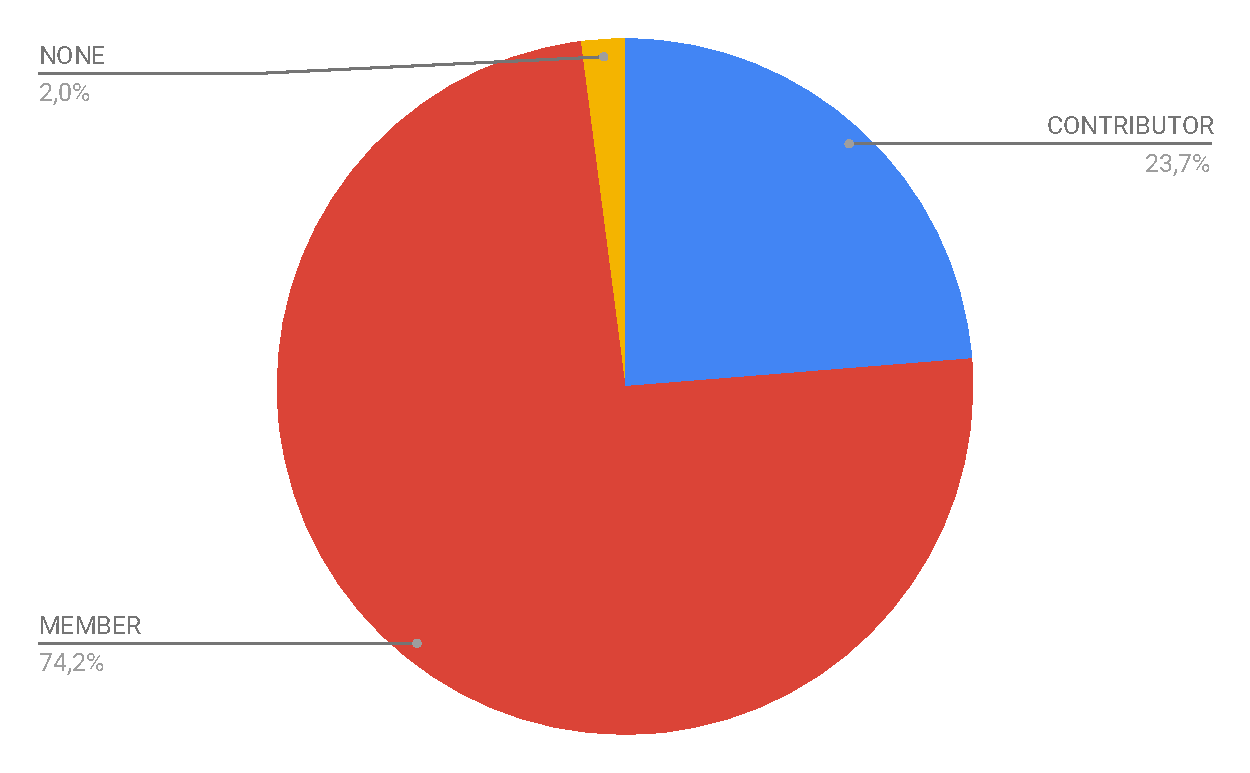
\includegraphics[width=\textwidth]{resultados/dist-author-type-node}
           \caption[Node.js]%
           {{\small Node.js}}
           \label{fig:dist-author-type-node}
       \end{subfigure}
       \hfill
       \begin{subfigure}[b]{0.475\textwidth}
           \centering
           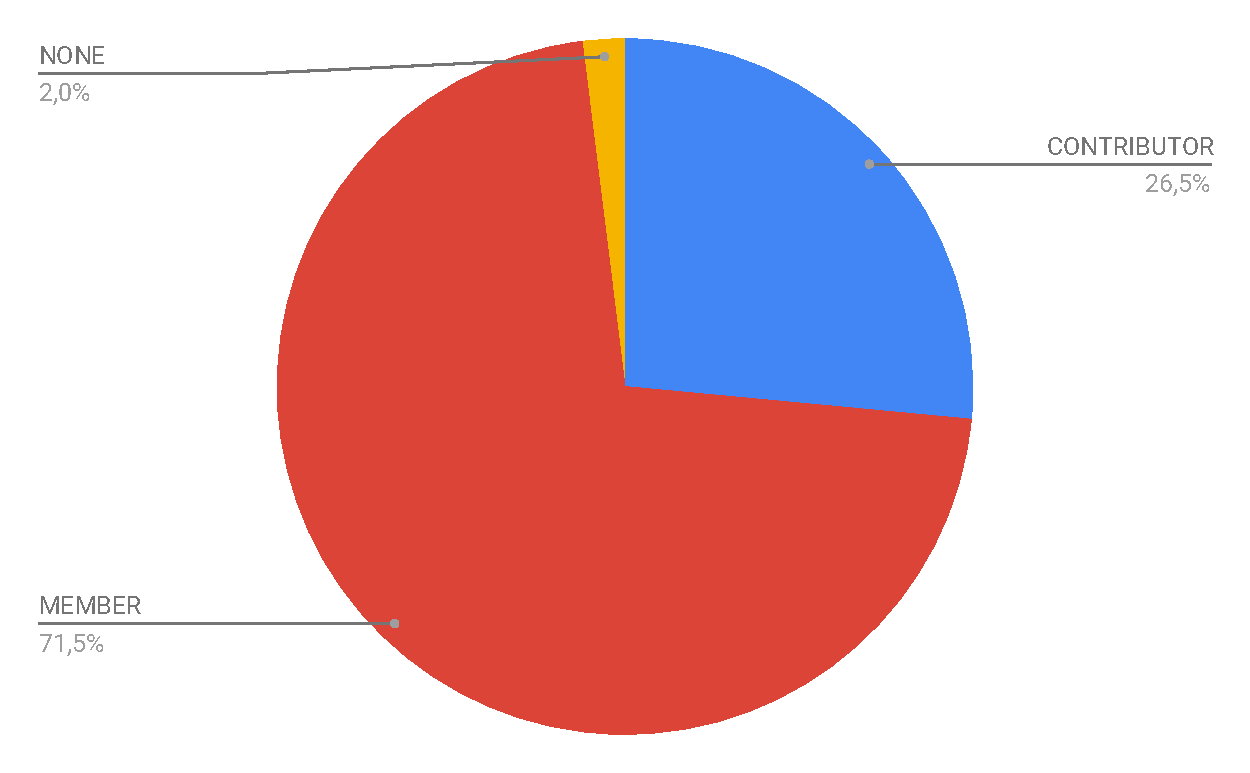
\includegraphics[width=\textwidth]{resultados/dist-author-type-symfony}
           \caption[Symfony]%
           {{\small Symfony}}
           \label{fig:dist-author-type-symfony}
       \end{subfigure}
       \vskip\baselineskip
       \begin{subfigure}[b]{0.475\textwidth}
           \centering
           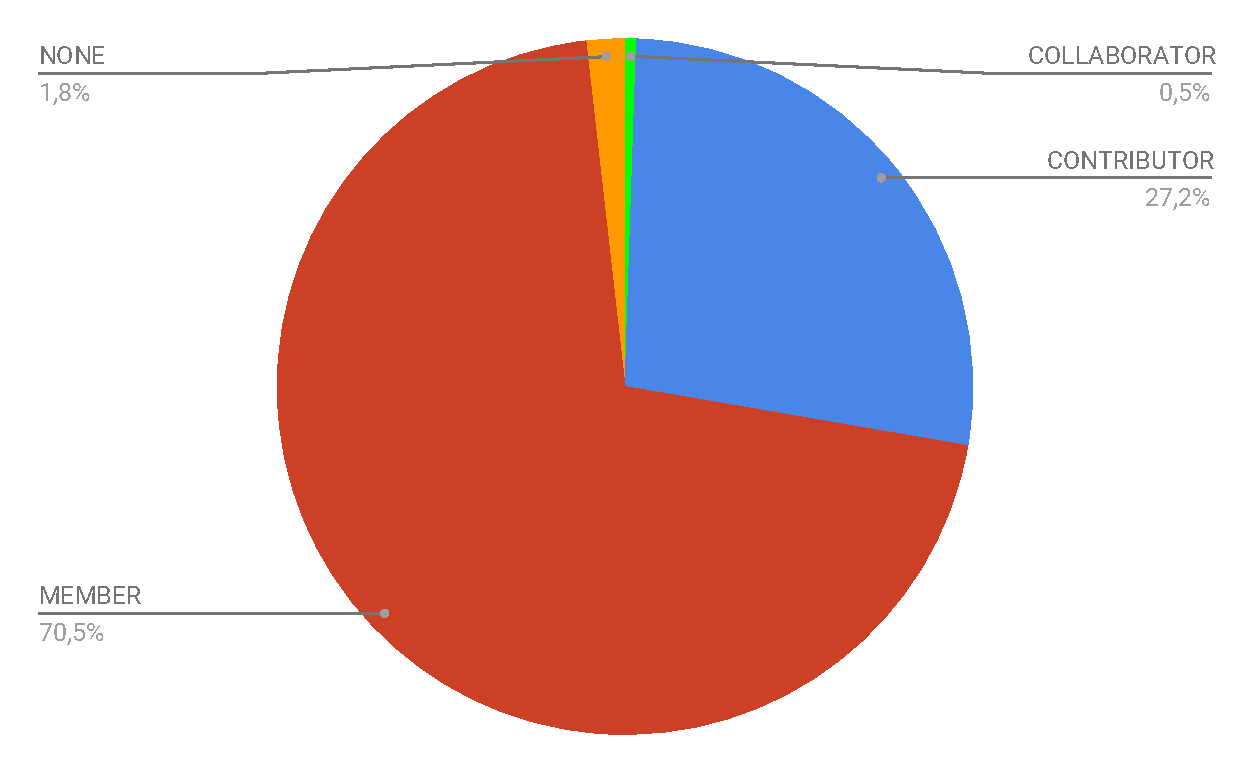
\includegraphics[width=\textwidth]{resultados/dist-author-type-kubernetes}

           \caption[Kubernetes]%
           {{\small Kubernetes}}
           \label{fig:dist-author-type-kubernetes}
       \end{subfigure}
       \quad
       \begin{subfigure}[b]{0.475\textwidth}
           \centering
           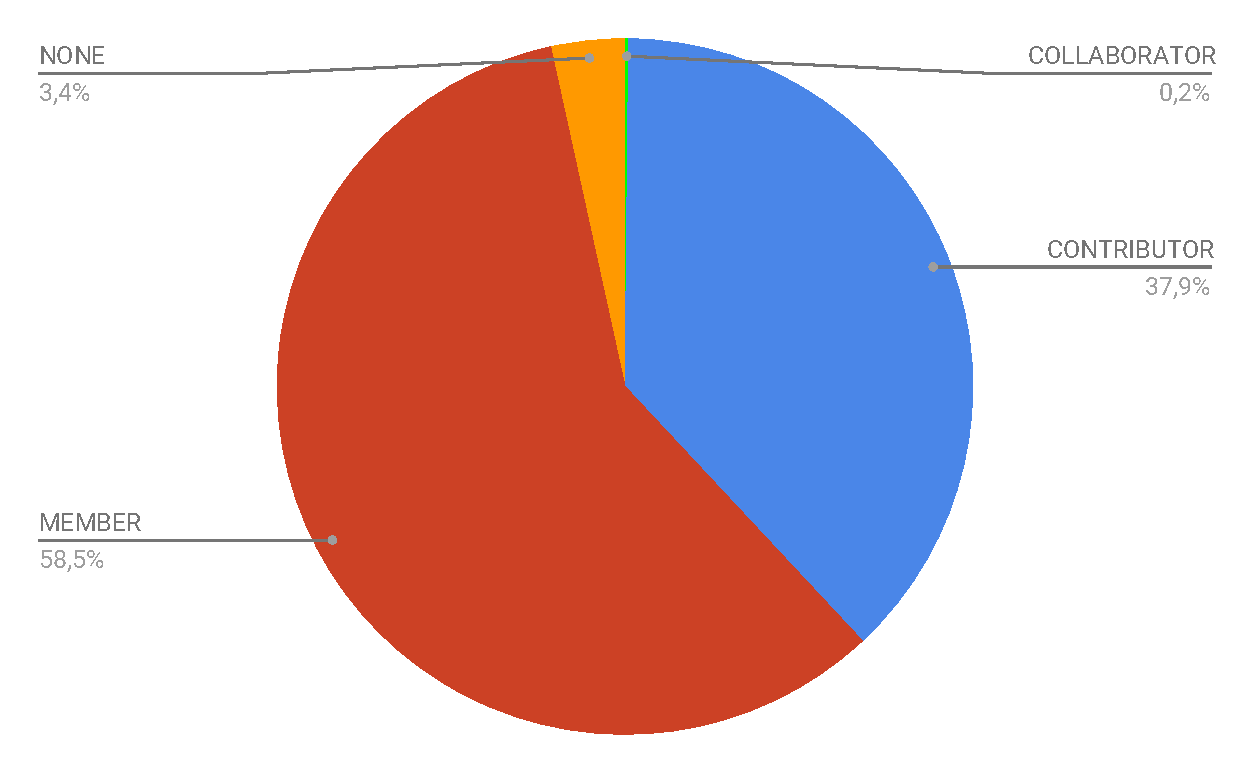
\includegraphics[width=\textwidth]{resultados/dist-author-type-tensorflow}
           \caption[Tensorflow]%
           {{\small Tensorflow}}
           \label{fig:dist-author-type-tensorflow}
       \end{subfigure}
       \caption[]
       {\small Categorias de autores responsáveis pelas interações nos projetos observados.}
       \label{fig:dist-author-type}
   \end{figure}


Assim, ao invés de indicar apenas os \textit{cores}, este método indica indivíduos na seguinte ordem de prioridade:

\begin{enumerate}
  \item Aqueles com maior influência sobre o autor nas \textit{labels} do \textit{``pull request''};
  \item os principais influenciadores nas \textit{labels} do \textit{``pull request''} de maneira global no projeto.
\end{enumerate}

  Ou seja, se $k$ for menor que o tamanho do conjunto dos revisores regidos pelo item 1, apenas desenvolvedores com histórico de interação com o autor e conhecimento nos tópicos necessários serão indicados. Nos casos dos revisados pela primeira vez, os indicados ao menos serão especialistas na categoria na qual o \textit{``pull request''} se insere. A única restrição é que o autor escolha as \textit{labels} antes de solicitar pelos revisores, o que pode ser facilmente adotado como uma política de contribuição dos projetos. O método é descrito através do algoritmo~\ref{alg:labelpartners}. A verificação de influência em determinadas tags utiliza a mesma equação~\ref{eq:penalization} de instanciação da rede, só que retorna pesos distintos para cada uma das \textit{labels} que compõe a relação entre dois nós.

  \begin{algorithm}

   \caption{Recomendação de revisores através do método LabelPartners}\label{alg:labelpartners}

       \Entrada{int $k$}
       \Entrada{string $login$}
       \Entrada{int $pr_id$}
       \Saida{$set_k$ de revisores recomendados}
       \Inicio{
           set $labels$ = get\_labels($pr\_id$)\;
           set $partners$ = $get\_partners(login, labels)$\;
           \eSe{$size(partners) < k$}{
           int $j$ = $k - size(partners)$\;
           set $extra = () $\;
             \Para {$label$ \textbf{in} $labels$} {
                  $extra.append(get\_experts(label)$)\;
             }
              $extraNotPartner = extra - partners$\;
              \Se{$extraNotPartner > j$}
              {
                $extra = (random\_sample$($extra, j))$\;
              }
           }
           {$partners = random\_sample(partners, k)$}
           \textbf{return} $partners + extra$\;
          }
  \end{algorithm}

Além de evitar os casos negativos dos algoritmos anteriores, o LabelPartners permite a ordenação das recomendações na saída. Ou seja, é possível que o conjunto que atende o primeiro caso (com interação direta com o autor no passado) seja ordenado por exemplo pela média do peso destas interações. O segundo conjunto também pode ser ordenado, onde o maior especialista nas \textit{labels} viria primeiro. Na linha $14$, o valor retornado corresponde a união dos conjuntos selecionados, sempre de tamanho $k$. Para evitar que indivíduos já indicados o sejam novamente, na linha $10$ é excluída a interseção entre os grupos já indicados e os \textit{cores}, de maneira análoga ao executado no algoritmo~\ref{alg:coresamecluster}.

\subsection{Resumo dos métodos}
Os métodos foram propostos de acordo com recomendações de trabalhos pregressos em relação ao uso de dados de colaboração e análises de redes sociais (SNA) \cite{fu2017, xia2017} <<citar revisão sistemática>>. Tais diretrizes condizem com os objetivos do trabalho de indicar revisores que aumentem a colaboração no contexto alvo. As abordagens foram concebidas não com a meta de se tornarem concorrentes, mas sim de se complementarem para cobrir particularidades dos projetos, mesmo que inseridos no mesmo contexto. Para avaliação dos métodos, foi desenvolvido um framework para aferir as métricas clássicas da área e especialmente os aspectos que tratam sobre a qualidade da revisão de código, cobertos na seção~\ref{sec:avaliacao_review}. Detalhes da implementação da ferramenta de avaliação e de recomendação são o tema do próximo capítulo.


\chapter{SOLUÇÃO DESENVOLVIDA}\label{chap:solucao}
    A solução desenvolvida engloba a automação das tarefas de instanciação, download e avaliação dos métodos, bem como a ferramenta de recomendação baseada nos métodos propostos. Levando em consideração os modelos atuais de revisão de código exploradas na seção~\ref{sec:code_review} são propostos os seguintes requisitos funcionais da ferramenta:
		\begin{itemize}
			\item Dada uma revisão de código, a ferramenta deve apresentar sugestões de pares técnicos para o o papel de revisor;
			\item o tamanho da lista deve ser escolhido pelo operador da ferramenta;
			\item os perfis dos indicados devem estar acessíveis (via link).
		\end{itemize}


		Os requisitos não funcionais estão relacionados às caracterísitcas técnicas da ferramenta que suportam os requisitos funcionais, como por exemplo disponibilidade, portabilidade e manutenibilidade. Dentre tais aspectos, pode-se destacar como mais relevantes:
	\begin{itemize}
		\item Interoperabilidade
		\begin{itemize}
			\item A ferramenta proposta deve-se comunicar o repositório de código fonte e ser compatível diferentes IDEs .
		\end{itemize}
		\item Manutenibilidade
		\begin{itemize}
			\item Existem diversas ferramentas de mercado para revisão, além de ferramentas de repositório de código fonte. Por isso a ferramenta deve ser modelada para permitir evoluções futuras que permitam a agregação de novas integrações que sejam importantes em outros domínios, como por exemplo software proprietário.
		\end{itemize}
    \item Portabilidade
    \begin{itemize}
      \item A ferramenta deve funcionar em diferentes sistemas operacionais e de forma auto contida, independente de instalação prévia de tecnologias.
    \end{itemize}
    \item Usabilidade
    \begin{itemize}
      \item As principais funcionalidade de recomendação da ferramenta devem estar disponíveis em interface web para operação sem necessidade conhecimento técnico avançado.
    \end{itemize}
	\end{itemize}


    Além dos requisitos funcionais e não funcionais caracterizados para atender os objetivos da pesquisa, é importante observar questões relativas á reprodutibilidade e avaliação do estudo. Ao conduzir as etapas de desenvolvimento e modelagem da arquitetura da ferramenta, é possível aderir a determinadas recomendações da literatura para agregar a capacidade do experimento de ser replicado, corroborado e estentido por pesquisas futuras. A próxima seção apresenta como tais aspectos foram levados em consideração.

    \section{Aspectos de Reprodutibilidade}

    Cada uma das tecnologias apresentadas é encapsulada através da tecnologia de virtualização Docker\footnote{https://www.docker.com/}. esta abordagem é uma resposta às iniciativas de reprodutibilidade na ciência, buscando maior transparência, confiabiliade e possibilidade de extensão nos experimentos \cite{freire2012}. Os três componentes (banco de dados relacional, orientado a grafo e os scripts de extração, transformação e carga) são encapsulados em contâiners distintos, como mostra a figura~\ref{fig:docker-model}.

    \begin{figure}[!htbp]
     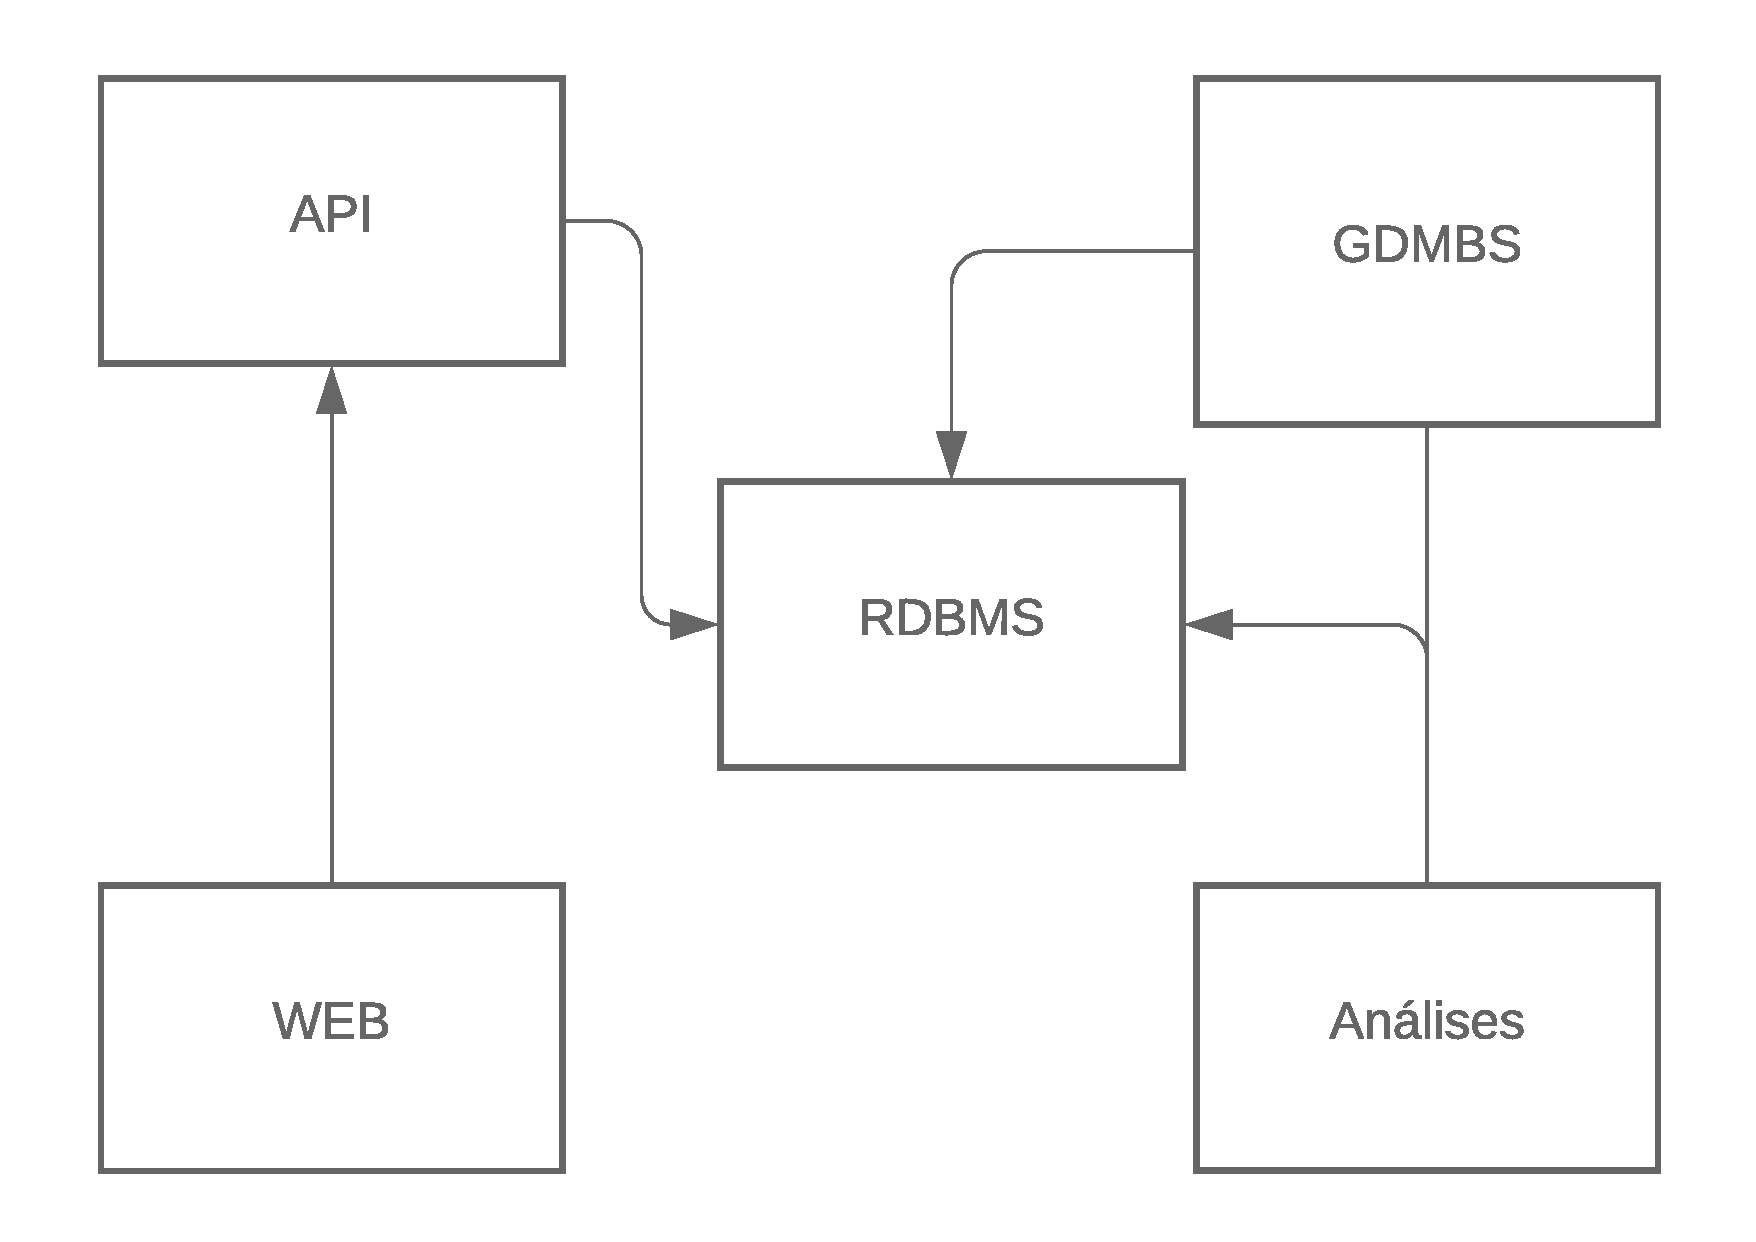
\includegraphics[width=.7\textwidth]{docker-model}
     \caption{Modelo de contâiners}\label{fig:docker-model}
    \end{figure}

    Os componentes WEB e API se comunicam para oferecer a interface de operação da ferramenta para os usuários. A fonte de dados para todas as execuções é o Sistema Gerenciador de Banco de Dados Relacional (RDMBS), apoiado pela estrutura orientada a grafos (GDBMS). O contâiner das análises fica responsável executar os métodos de recomendação, otimização, ETL e outros que apoiam a descoberta de conhecimento na plataforma. Mais detalhes sobre cada um dos contâiners e suas funcionalidades estão descritos na seção~\ref{sec:arquitetura} e \ref{sec:funcionalidades}. Estes componentes são orquestrados através do docker-compose\footnote{https://docs.docker.com/compose/}, que configura os parâmetros e acessos necessários para o funcionamento do sistema sem que o usuário precise realizar nenhuma ação extra.

    Com um conjunto grande de dependências, tecnologias e minúncias que estão envolvidas neste tipo de experimento, o código fonte e a descrição ainda que detalhada dos dados não é suficiente para alcançar níveis adequados de reprodutibilidade~\cite{ince2012}. Com auxílio dos containers Docker, é possível criar instâncias executáveis dos experimentos que vão funcionar em diferentes computadores, arquiteturas e situações, sem necessidade de conhecimento técnico por parte do executor das tecnologias utilizadas \cite{boettiger2015}.

    De acordo com Sinha et al. \cite{sinha2016}, a maturidade da reprodutibilidade de um experimento científico computacional pode ser medido de acordo o nível dos seguintes aspectos que foram trabalhados em sua disponibilização. A figura~\ref{fig:espectro_reprodutibilidade} mostra o espectro de reprodutibilidade, que encara esta característica como um constante trabalho de evolução não binário, podendo uma pesquisa se tornar mais ou menos reprodutível ao se utilizar determinadas técnicas. A figura~\ref{fig:escala_reprodutibilidade} mostra o detalhamento de cada aspecto que contribui para que esta característica seja evidenciada.

    \begin{figure}[!htbp]
     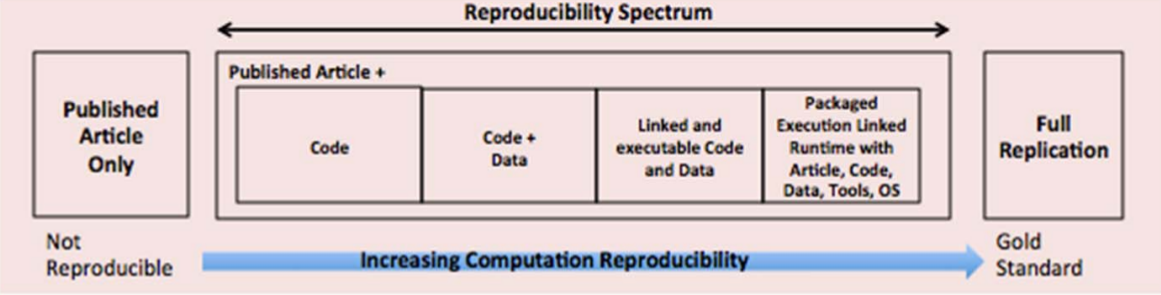
\includegraphics[width=\textwidth]{espectro_reprodutibilidade}
     \caption{Espectro de Reprodutibilidade}\label{fig:espectro_reprodutibilidade}
    \end{figure}

    \begin{figure}[!htbp]
     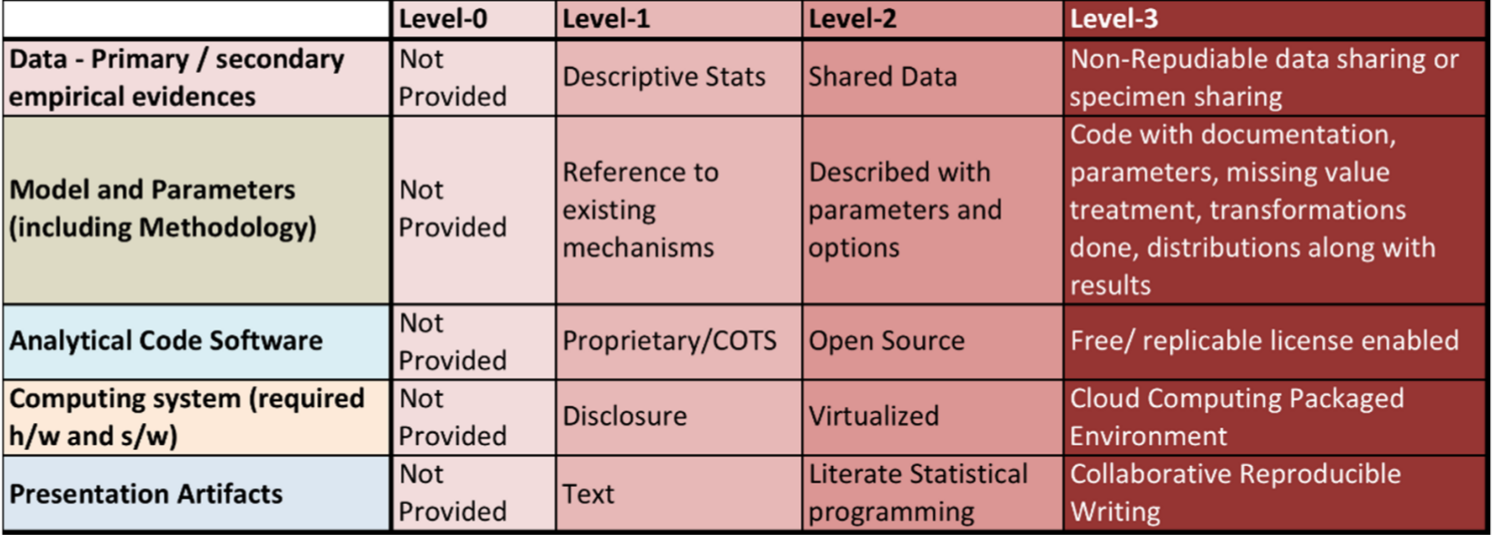
\includegraphics[width=\textwidth]{escala_reprodutibilidade}
     \caption{Escala de Maturidade de Reprodutibilidade}\label{fig:escala_reprodutibilidade}
    \end{figure}


    \subsection{Dados - Evidências Primárias/Secundárias} Esta categoria analisa a disponibilidade dos dados utilizados para futuros pesquisadores. Pode variar de simplesmente não dispobilizado até a disponibilização íntegra das informações, valendo-se de meios para uma oferta não repudiável e com garantias de integridade e veracidade. Neste trabalho, todos os dados (em suas diferentes agregações) são disponibilizados para uso futuro. Além disso os mecanismos de extração são automatizados, permitindo buscar outros projetos ou atualizar os dados existentes. Como não há garantias de não repúdio e autenticação dos dados, o estudo se classifica como nível 2 nesta categoria.

    \subsection{Modelo e Parâmetros} Verificação dos modelos e parâmetros utilizados no experimento. São essenciais para a discussão e reprodução do experimento, além de qualquer tentativa de otimização. Varia de não disponibilizado até a disponibilização plena com documentação adequada, interface robusta que trate valores fora do domínio (como nulos) e também prática, facilitando os testes com parâmetros e dados distintos. Os modelos de dados e de execução são detalhados neste trabalho. Além disso, todas as análises são automatizadas e encapusladas através de comandos executáveis dentro de um contâiner Docker. Por conseguinte, o trabalho pode ser classificado como nível 3 nesta categoria

    \subsection{Código Fonte} Disponibilidade do código fonte utilizado nas análises. Pode variar de não disponível (proprietário) até open source com direito de extensão e modificação. Neste projeto todo o código fonte é opensource e disponibilizado sob a permissiva licença MIT~\cite{mit}, categorizando assim o nível 3.

    \subsection{Sistema computacional requerido} Detalhamento das informações de hardware e software necessários, como por exemplo memória, arquitetura, processador, versão e plataforma. O nível ideal é a disponibilização do experimento em ambiente virtualizado em nuvem, em arquitetura que permita tanto a reprodução "as is" quanto extensão e modificação de parâmetros e dados de entrada. Como todo o pipeline deste projeto está disponibilizado na infraestrutura Docker, a única restrição da máquina do pesquisador é ter o Docker instalado. Em adição, serviços de nuvem como a Amazon AWS fornecem infraestutura para execução de containers Docker sem necessidade de configurações extras. Informações do hardware utilizado nos experimentos estão disponibilizadas nas próximas seções. Assim, o projeto pode ser classificado como nível 3 nesta categoria.

    \subsection{Artefatos de apresentação}

    Todos os artefatos de apresentação, tais como artigos, dissertação e posters oriundos deste trabalho foram construídos com o \LaTeX \cite{lamport1994} e o código fonte disponibilizado. Gráficos e tabelas foram produzidos diretamente através de scripts e/ou com ferramentas \textit{Open Source}, como o Gephi\footnote{https://gephi.org/}. Nesta categoria o estudo também se caracteriza como nível 3.

    De acordo com a escala proposta \cite{sinha2016} e com as informações prestadas nesta seção, concluímos que a pesquisa está no nível 2 de maturidade em reprodutibilidade, já que o autor propõe que o trabalho seja classificado de acordo com a menor nível atingido em uma das categorias.

    \section{Arquitetura}\label{sec:arquitetura}

		A ferramenta proposta é estruturada em diferentes componentes, de acordo com sua função e tecnologias escolhidas. A figura~\ref{fig:componentes} mostra essa divisão, onde os quatro principais componentes possuem subcomponentes com tarefas mais específicas autocontidas. As subseções seguintes tratam de cada um dos componentes em particular.


    \begin{figure}[!htbp]
        \centering
        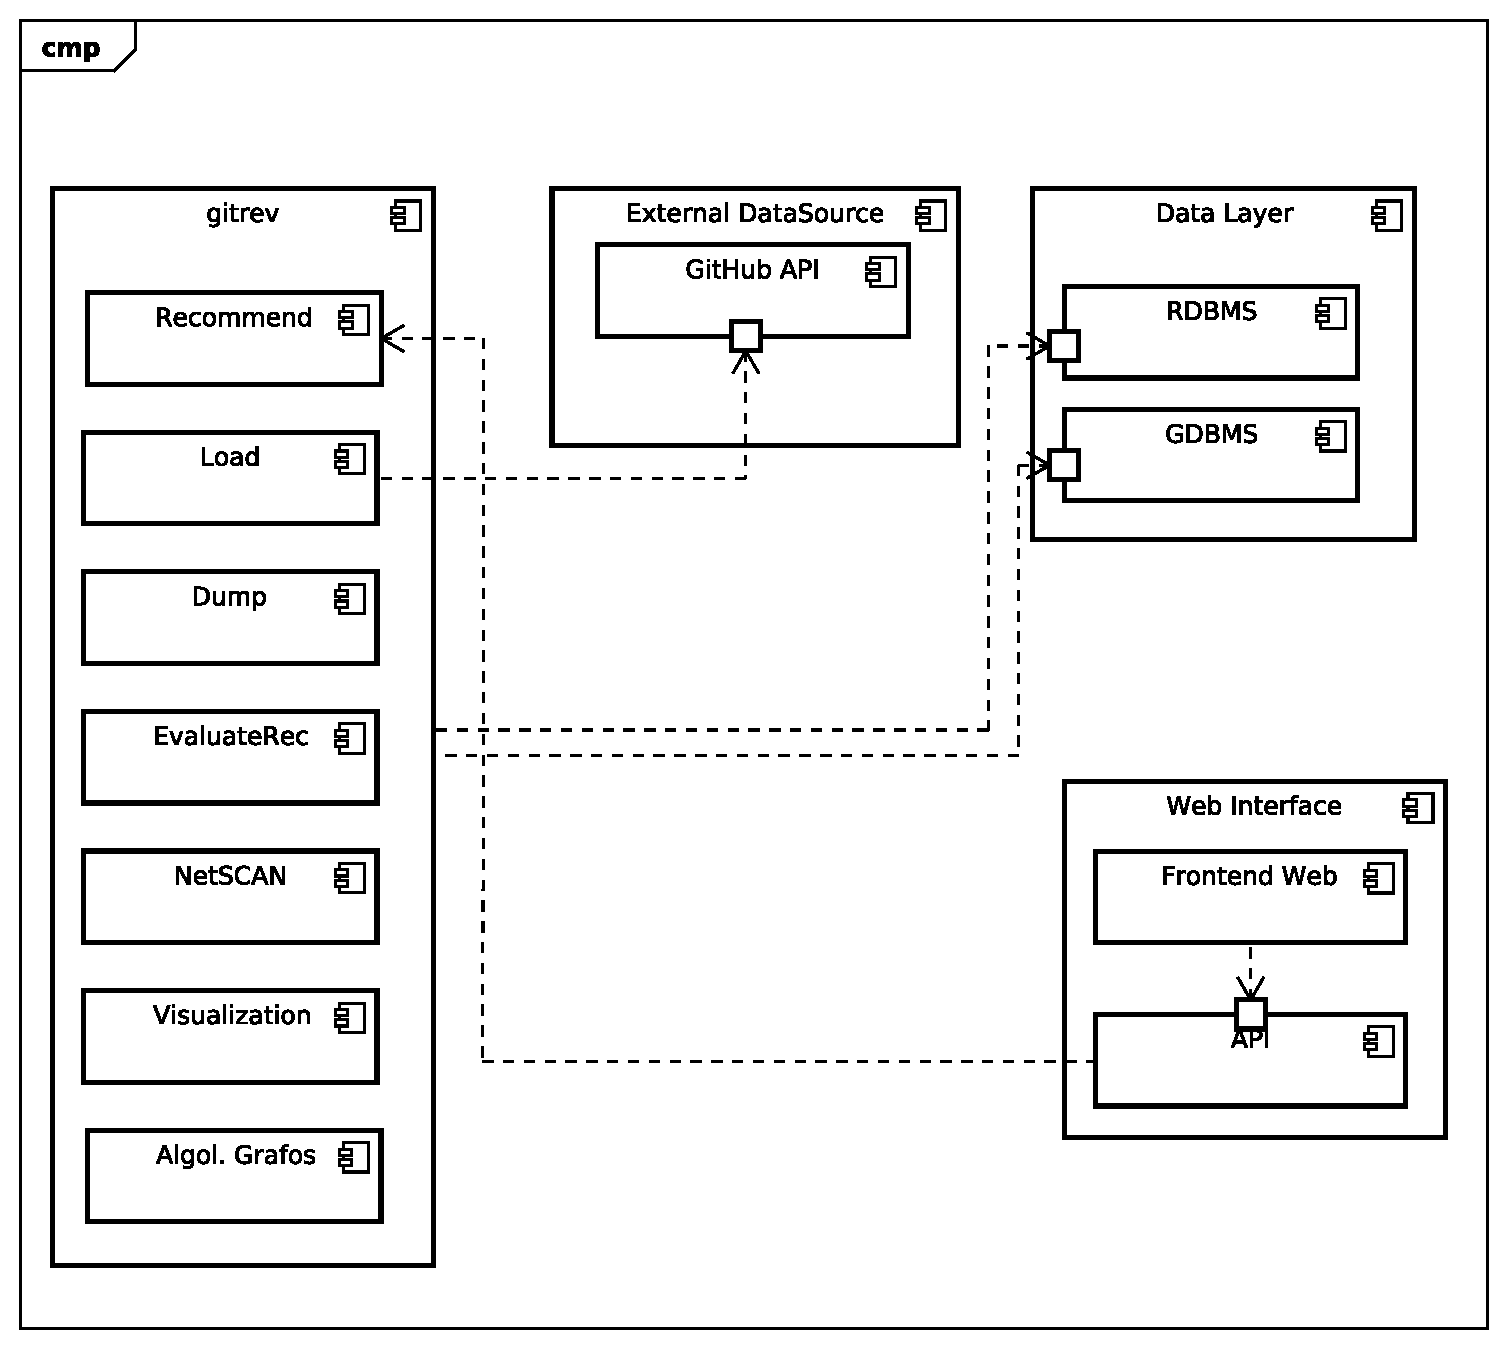
\includegraphics[width=.8\textwidth]{componentes}
        \caption{Diagrama de Componentes da Ferramenta}\label{fig:componentes}
    \end{figure}

    \subsection{External DataSource}

    O módulo de dados externo é incorporado pela API do GitHub, fonte dos dados brutos extraídos e armazenados no componente de persistência de dados. A versão estável para integração foi a v3, que implementa o padrão arquitetural RESTful\cite{fielding2002}. Existe a API em recém lançada v4\footnote{https://developer.github.com/v4/}, que utiliza da especificação GraphQL para exposição dos serviços. Esta não foi utilizada devido a documentação ainda recente e pela preferência ao padrão REST.

    \subsection{Data Layer}

    Neste componentes os dados normalizdos oriundos do GitHub são persistidos e tidos como base para as outras funcionalidades existentes. o Diagrama de Entidade Relacionamento (DER) na figura~\ref{fig:der} representa as informações disponíveis. As colunas salvas são as mesmas que a API do GitHub disponibiliza e foram restringidos pensando no espaço, já que só a entidade \textit{``pull request''} tem 37 campos. Todas as tabelas possuem um identificador (id) gerado sequencialmente, além das informações de identificação do próprio GitHub.  O DBMS escolhido para este componente foi o PostgreSQL 10.5, que é \textit{``Open Source''} e implementa as características do padrão ACID~\cite{gilbert2002} de atomicidade, consistência, isolamento e durabilidade.

    \begin{figure}[!htbp]
     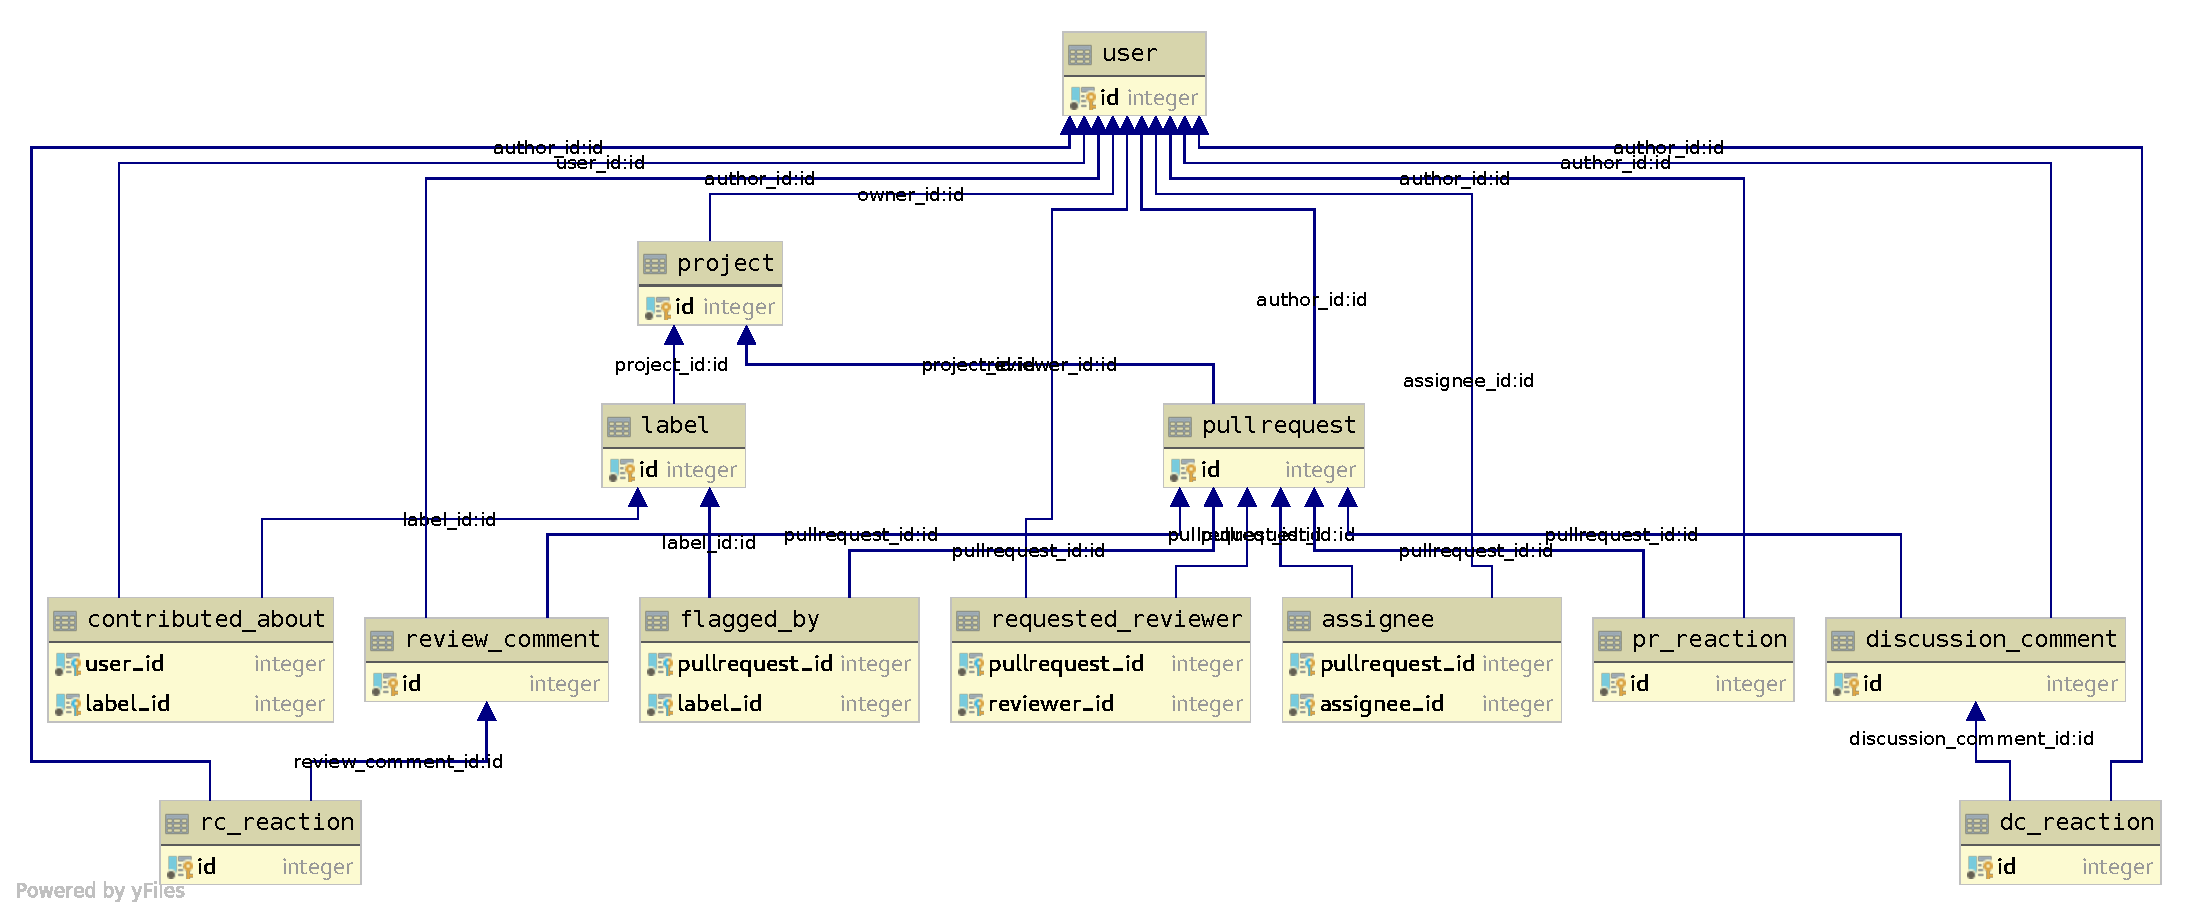
\includegraphics[width=\linewidth]{der}
     \caption{ Diagrama de Entidade Relacionamento (DER)}\label{fig:der}
    \end{figure}

    Na figura~\ref{fig:der} é possível ver que a entidade \textit{user} é compartilhada em diferentes projetos, e assume o papel de autor de várias outras. Isso significa que mesmo que um autor contribua em projetos diferentes será representado uma única vez, o que permite análises mais complexas entre projetos distintos. Os \textit{``pull requests''}, outra categoria chave para as análises, possui dois tipos de comentários: aqueles feitos no formato de discussão (\textit{discussion\_comment}) e aqueles que apontam para partes específicas do código (\textit{review\_comment}). A segunda categoria que é utilizada neste trabalho. Estes comentários (e o próprio \textit{``pull request''}) recebem as respectivas reações, utilizadas como representações de sentimentos positivos ou negativos em relação às interações. Os \textit{``pull requests''} se relacionam \textit{n:m} com as \textit{labels}, indicando as categorias nas quais foram classificados. A tabela \textit{requested\_reviewer} representa solicitações de revisores que quando aceitas viram registros na tabela \textit{assignee}. Estes dados não foram utilizados para avaliar a recomendação porque apenas os indivíduos com permissão são referenciados como ``atribuídos'', o que iria enviesar os resultados das recomendações de \textit{cores}.

    O segundo componente da camada de persistência é a rede de desenvolvedores instânciada em um Sistema Gerenciador de Banco de Dados Orientado a Grafos (GDBMS), que disponibiliza os dados relevantes do modelo relacional na visualização de grafos, permitindo as análises e métodos de clusterização serem executados com maior facilidade. A tecnologia escolhida neste caso foi o Neo4j\footnote{https://neo4j.com/} que além de possuir o plugin do NetSCAN permite a integração com o Gephi para produzir filtros, análises e visualizações mais elaboradas. Apenas os dados básicos dos indivíduos e suas relações foram instanciadas nele, enquanto consultas mais elaboradas precisam contar com o suporte do PostgreSQL.

    \subsection{Gitrev}

    Gitrev é o nome da plataforma e do principal componente do sistema, sendo responsável pela interação com os dados durante todo o processo. Todo o componente foi desenvolvido em Python, aproveitando da extensibilidade, ecossitema e flexibilidade da linuagem. A interface com o RDBMS é suportada pela biblioteca SQLAlchemy\footnote{https://www.sqlalchemy.org/}, sendo o pilar da camada de acesso aos dados (\textit{Data access objetcs}, ou DAO). Para a interação com o GDBMS a biblioteca Py2neo\footnote{https://py2neo.org/v4/} provê interface semelhante ao seu par relacional. O módulo \textit{Dump} inicia o processo de extração ao acessar a API do GitHub, com auxílio da biblioteca requests\footnote{https://2.python-requests.org/en/master/}. O algortimo de extração dos dados foi projetado com uma série de cuidados para garantir a integridade e disponibilidade das informações, diante das nuances do repositório e do domínio de dados. Os principais aspectos observados são:

    \subsubsection{Inconsistência nos dados} Para evitar dados inconsistentes, toda a extração é feita dentro de uma transaction relacional do RDBMS, garantindo que todas as ações serão executadas (ou canceladas) de forma atômica. As restrições de chave primária também são a primeira linha de defesa para evitar que informações inconsistentes sejam armazenadas (como por exemplo um comentário relacionado a um \textit{``pull request''} que não existe).

    \subsubsection{Tratamento das exceções da API} O repositório de dados pode se comportar de maneira anormal durante a extração dos projetos, por diversos motivos: indisponibilidade dos serviços, lentidão do cliente, problemas de conexão entre outros. Assim é necessário tratar erros (como 400, 500 e 502) e evitar que o dump seja interrompido. Para isso, as respostas são tratadas, e detectados erros temporários como estes, o request é agendado para se repetir em uma janela de tempo definida.

    \subsubsection{Ratelimit da API} A API do GitHub limita o número de requests a 5000/hora. Por isso, é necessário que o cliente controle o número de requests para que não seja bloqueado. Assim, o componente de extração limita o seu número de requests, entrando em espera quando o número se aproxima ao limite imposto.

    \subsubsection{Unicidade de usuários} Usuários são entidades espalhadas entre os diferentes projetos. Para possibilitar análises globais e estatísticas realísticas de tamanhos de projetos, é necessário que não haja duplicação entre os usuários. O componente de extração também garante que não hajam usuários duplicados.

    O módulo \textit{Load} é responsável por gerar a rede especificada na seção~\ref{sec:modelagem}, a partir dos dados encontrados no RDBMS. Além do peso relatado na definção do grafo, os pesos segregados por \textit{label} necessários para o algoritmo~\ref{alg:labelpartners} de recomendação já são introduzidos. Uma propriedade única é que o peso global de determinada relação é a média ponderada dos pesos por \textit{label}.

    O componente NetSCAN reúne as funcionalidades de criação, avaliação e otimização dos \textit{clusters}. Nele é possível encontrar a combinação de parâmetros que geram a melhor silhueta, como explicado na seção~\ref{subsec:netscan}. Os utilitários que avaliam a qualidade dos grupos detectados e sua relevância semântica em relação ao processo produtivo do projeto também são encapsuladas neste módulo. Muitas vezes tais análises são executadas com auxílio do módulo \textit{Algortimos de Grafos} onde consta um conjunto de métodos para avaliar as redes e os relacionamentos encontrados.

    Na camada \textit{Visualization} é possível encontrar os algortimos que se apóiam nas ferramentas matplotlib\footnote{https://matplotlib.org/index.html} e numpy\footnote{https://www.numpy.org/} para gerar gráficos de distribuição de grau, \textit{boxplot} das silhuetas entre outros.

    No componente \textit{Recommendation} são efetuadas as recomendações tendo como base os métodos propostos. As informações são extraídas e do GDBMS e disponibilizadas para o componente de interface com o usuário. A avaliação das recomendações é feita no módulo \textit{EvaluateRec}, que executa recomendações para revisões dentro de um período escolhido e as analisa de acordo com os parâmetros definidos. Este é também o responsável por avaliar a significância estatística das diferenças entre as abordagens, com apoio da biblioteca ScyPy\footnote{https://www.scipy.org/}.

    \subsection{Web Interface}

    A interface web é destinada à operação cotidiana da ferramenta em busca dos revisores adequados. A aplicação se estrutura em dois componentes. O \textit{backend} é provido pelo Flask\footnote{http://flask.pocoo.org/}, microframework com capacidade de dar suporte à interface RESTful modelada, e é acessado através de um proxy provido pelo servidor web Nginx\footnote{https://www.nginx.com/}. O backend acessa o componente \textit{Recommend} e os \textit{``pull requests''}  persistidos no RDBMS para responder às solicitações do \textit{frontend}. Este componente foi desenvolvido com o apoio do framework reativo Vue.js\footnote{https://vuejs.org/} e é representado na figura~\ref{fig:web-interface}. O componente de seleção dos \textit{``pull requests''} é dinâmico e realiza a busca de acordo com a entrada do usuário. Os links nos usuários levam aos seus perfis no GitHub.

    \begin{figure}[!htbp]
     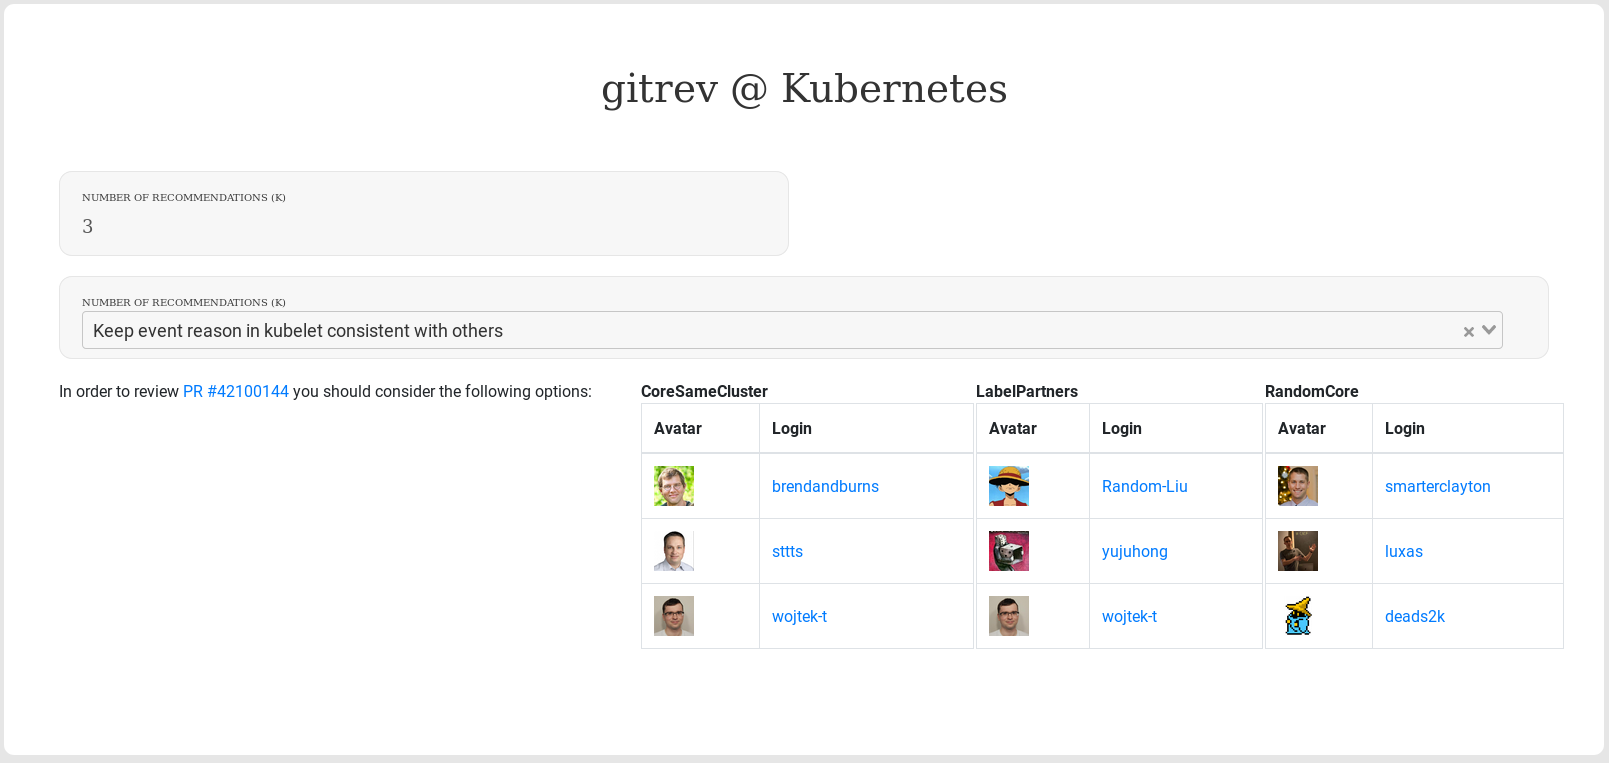
\includegraphics[width=\columnwidth]{web-interface}
     \caption{Funcionalidade de recomendação no projeto Kubernetes}\label{fig:web-interface}
    \end{figure}



   \section{Funcionalidades}\label{sec:funcionalidades}

   A utilização da ferramenta pode ser dividida em duas etapas principais: na preparação e na recomendação. A preparação pode ser executada de tempos em tempos, para atualizar a base oriunda do GitHub e testar novos parâmetros. É uma tarefa que pode ser agendada no processo de trabalho da organização e por isso é disparada via linha de comando (CLI). O diagrama de atividades na figura~\ref{fig:atividade} descreve o processo.

   \begin{figure}[!htbp]
    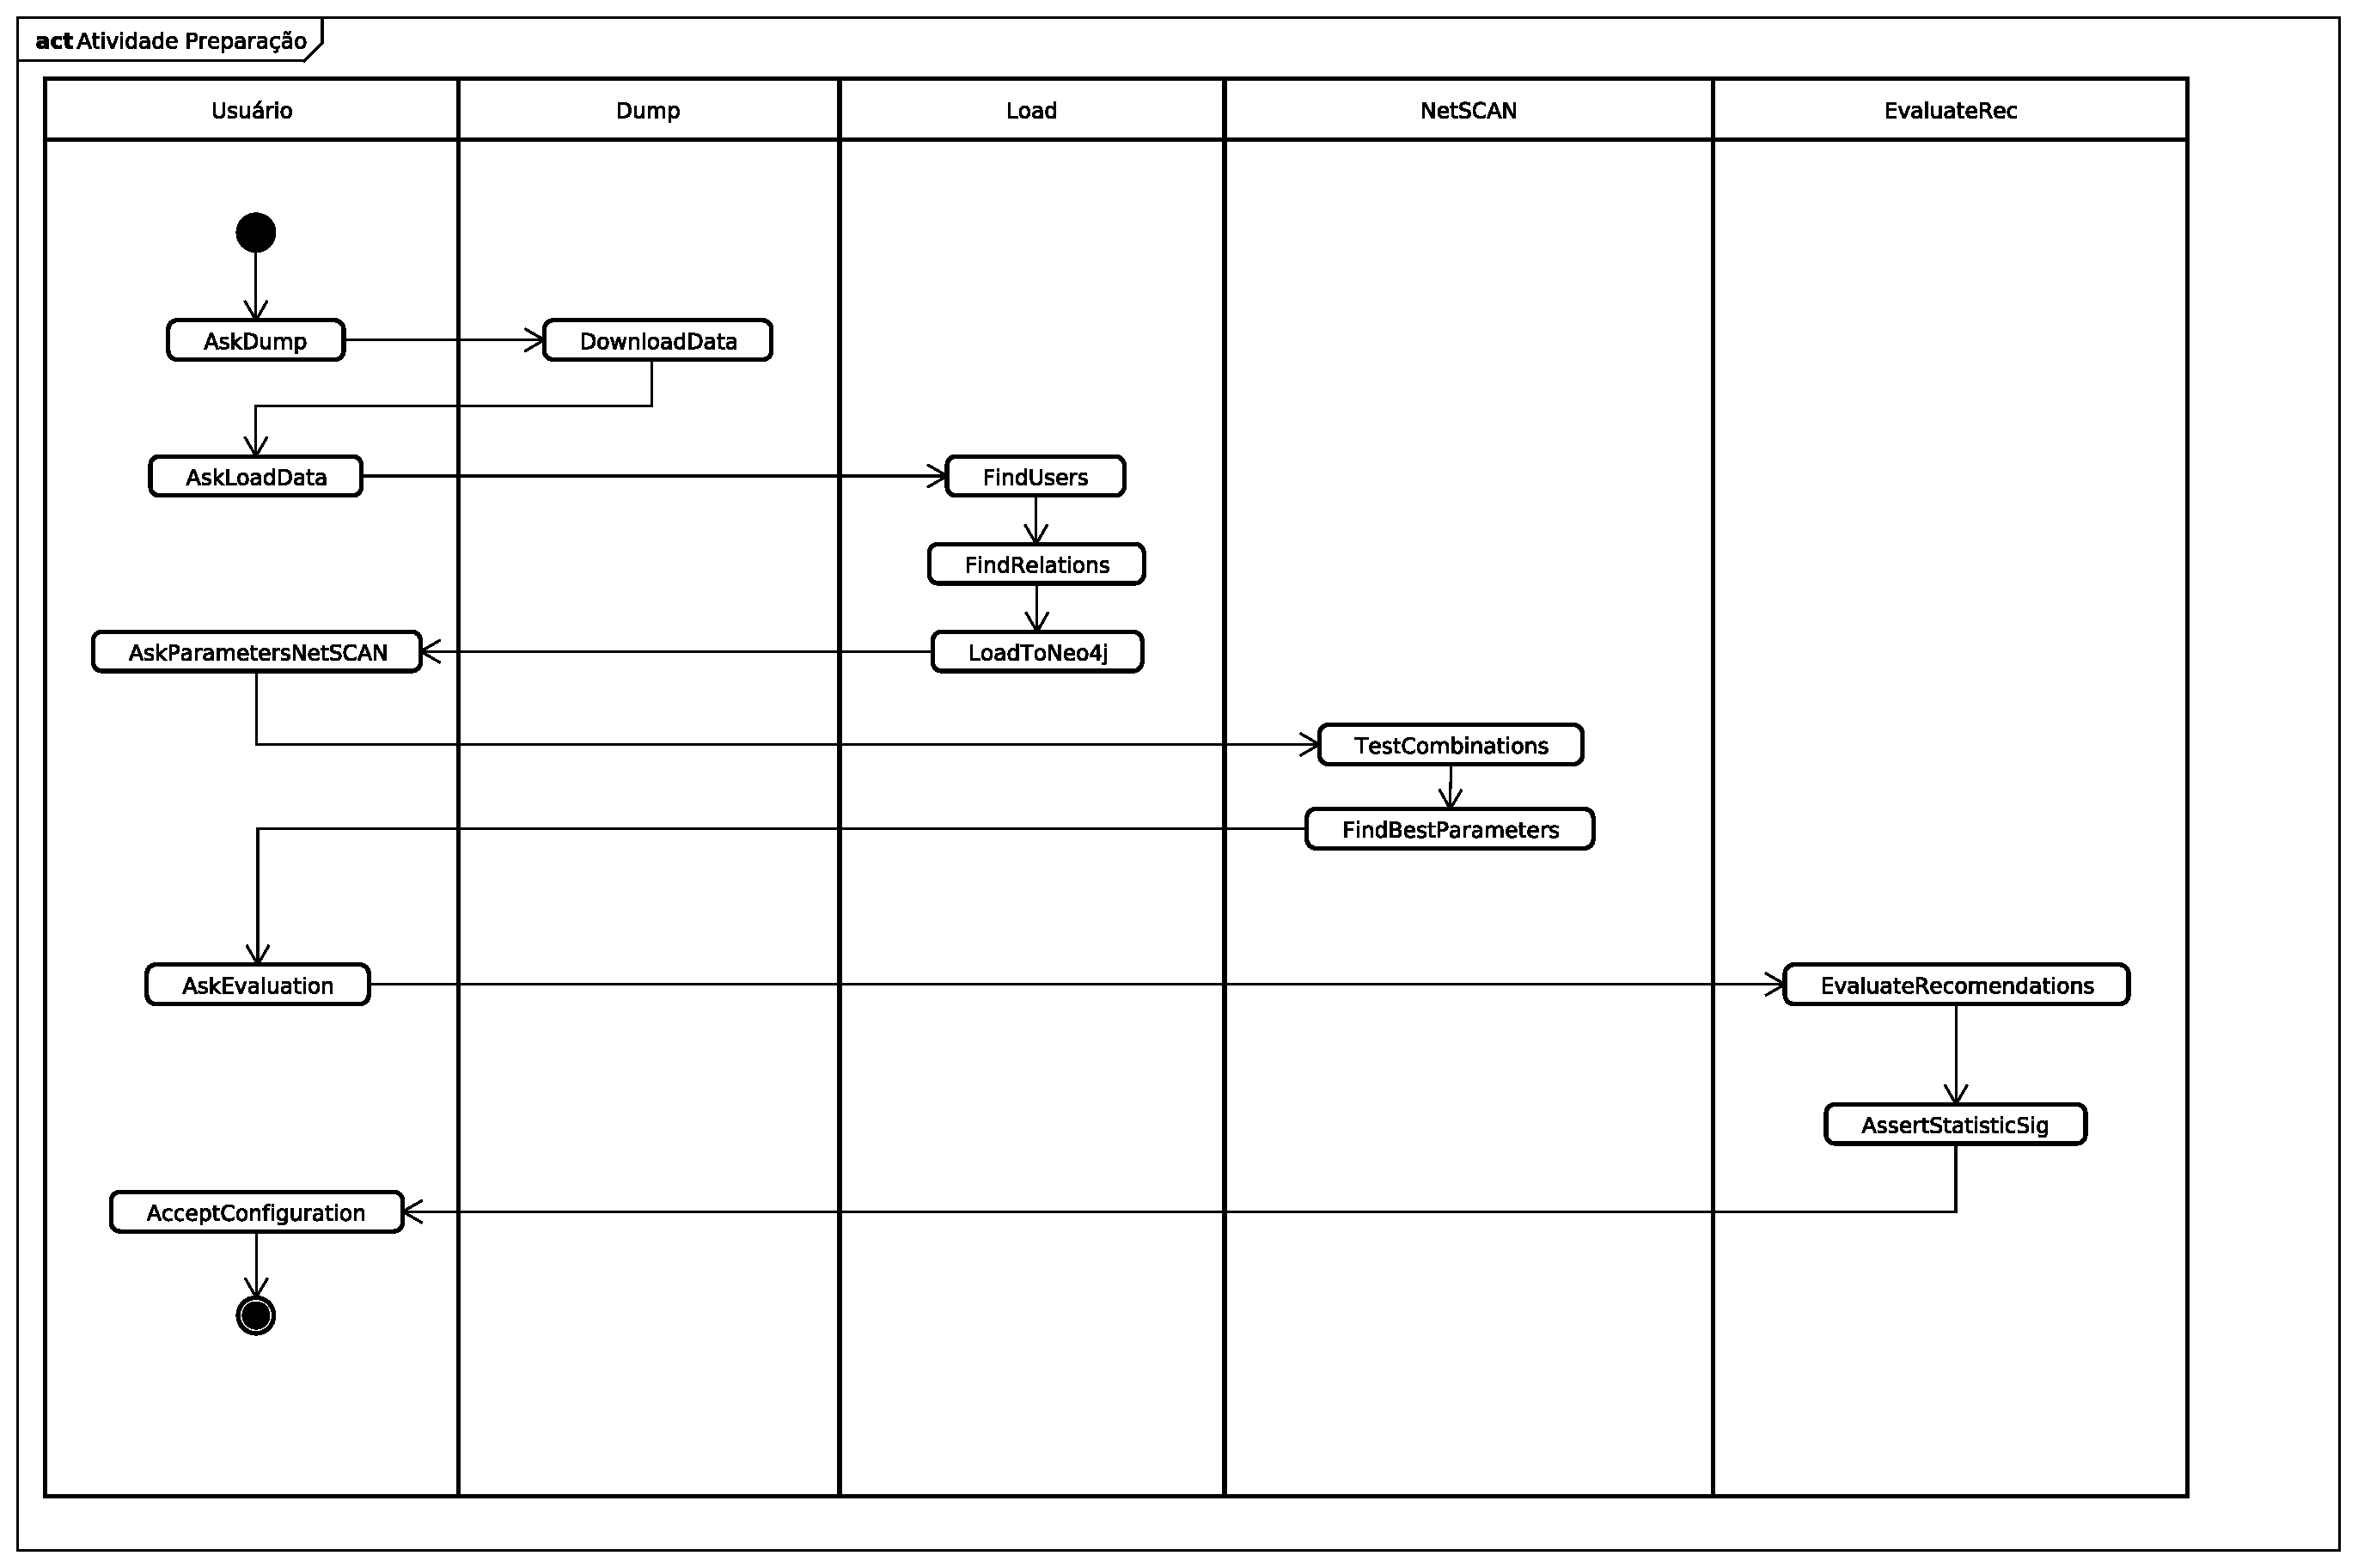
\includegraphics[width=\textwidth]{atividade}
    \caption{Diagrama Atividades - Preparação}\label{fig:atividade}
   \end{figure}

   O responsável deve solicitar o \textit{download} de um ou mais projetos, que serão extraídos via API. O RDBMS foi projetado para persistir dados de quantos projetos forem solicitados. Contudo cada instância do Neo4j representa, nesta versão, dados de apenas um projeto. O usuário então pode solicitar a \textit{clusterização} da rede, passo necessário para os algortimos de recomendação~\ref{alg:randomcore} e~\ref{alg:coresamecluster}. Os parâmetros utilizados podem ser obtidos através da otimização, ou salvos para utilização recorrente, caso seja assim preterido. Avaliação dos métodos é um passo opcional que pode ajudar o operador a escolher o melhor método para cada situação. Ao finalizar este fluxo, os usuários estão livres para solicitar as recomendações na plataforma web, o que também é possível através da interface de linha de comando \inlinecode{gitrev PULL\_REQUEST\_ID [k]}. O valor padrão de $k$, se não informado, é 1, indicando que apenas um revisor será recomendado.

   O fluxo de operação cotidiano ferramenta foi projetado visando compatibilidade com o processo de revisão, especialmente no modelo \textit{pull based} \cite{gousios2014} introduzido na seção~\ref{sec:pull_based}. A figura~\ref{fig:sequencia} representa o diagrama de sequência da comunicação entre o autor do \textit{``pull request''} (responsável pela escolha dos revisores), o GitHub e o utilitário de recomendação.

   \begin{figure}[!htbp]
    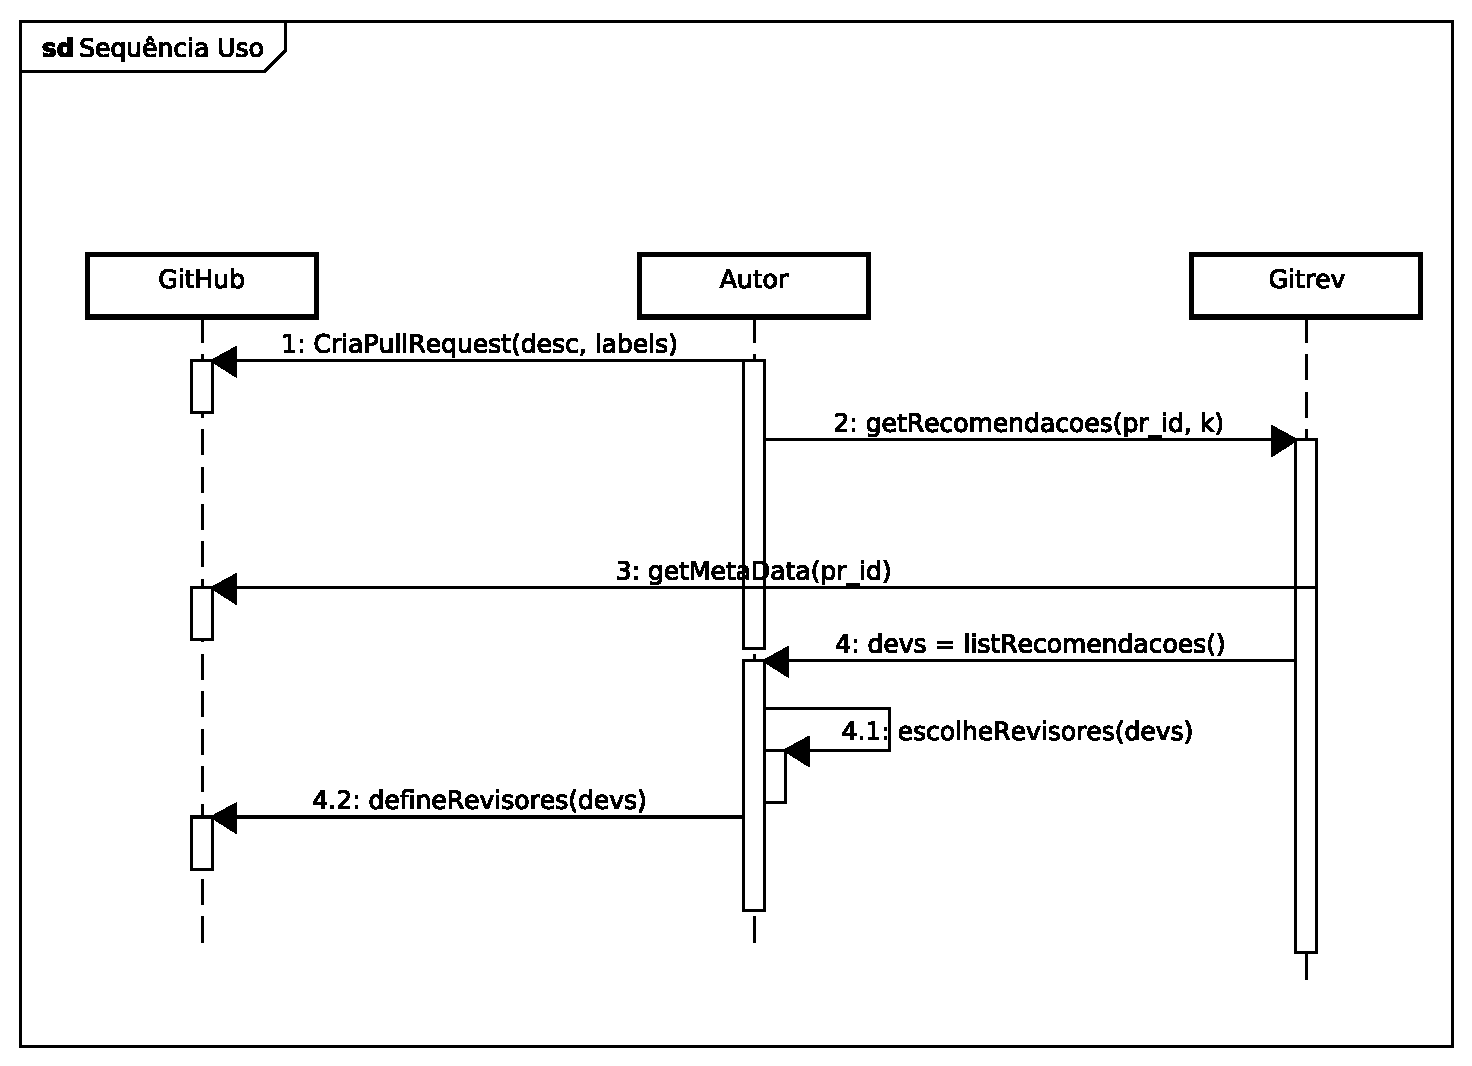
\includegraphics[width=\textwidth]{sequencia}
    \caption{Diagrama de Sequência da ferramenta - utilização}\label{fig:sequencia}
  \end{figure}

  O primeiro passo consiste no autor criar a revisão com os dados relevantes, como por exemplo descrição, link com issues solucionadas, dúvidas e possíveis discussões que estejam relacionadas ao código submetido. Ao executar o utilitário, este irá acessar os metadados do Github para encontrar outras revisões de contexto semelhante e extrair informações de revisores que estiveram envolvidos nelas. A partir daí a recomendação é feita e disponibilizada para o revisor, que poderá convidar um subconjunto da lista apresentada para o papel de revisor.

  Com a ferramenta dispondo do sistema de recomendação e de avaliação, é possível conduzir um processo para averiguar a pertinência dos resultados  de acordo com os objetivos deste trabalho. O processo de avaliação é descrito no próximo capítulo.

\chapter{AVALIAÇÃO DA SOLUÇÃO}\label{chap:resultados}
    A avaliação da solução proposta passa por três etapas distintas: a extração dos dados, a preparação das estruturas e a apreciação das métricas escolhidas e a significância estatísitica dos resultados. A figura~\ref{fig:avaliacao} mostra o procedimento.

     \begin{figure}[!htbp]
       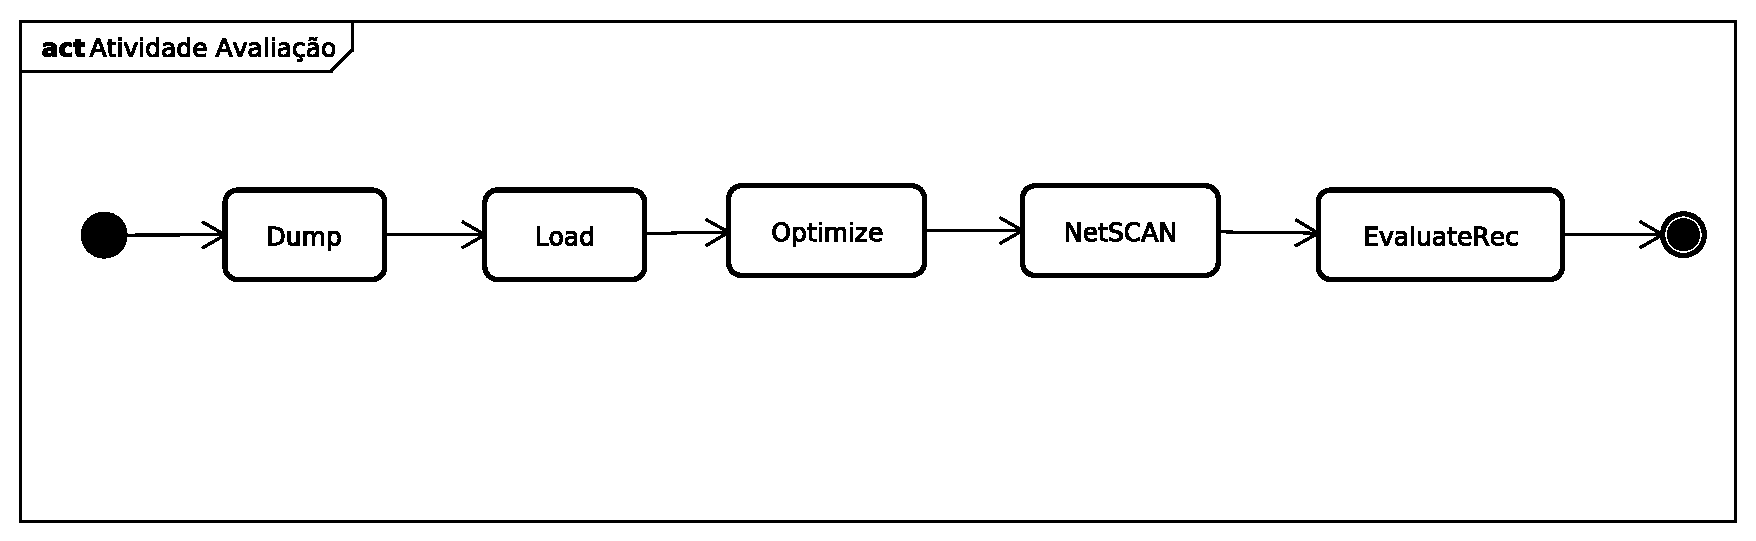
\includegraphics[width=\textwidth]{avaliacao}
      \caption{Processo de avaliação}\label{fig:avaliacao}
    \end{figure}

    As atividades estão todas contidas na ferramenta, com uma ordem de execução similar ao uso exemplificado na seção~\ref{sec:funcionalidades}. A partir dos dados extraídos relativos aos 4 projetos selecionados na subseção~\ref{subsec:escolhaprojetos}, as respectivas redes são construídas. É possível escolher o intervalo de tempo para limitar quais dados serão utilizados no processo. Tal mecanismo serve para possibilitar que os dados utilizados na avaliação sejam diferentes dos utilizados para criar a rede, diminuindo o risco de viés nas análises, sem ter que acessar novamente a API do GitHub. A otimização dos parâmetros pode ser feita uma única vez e aproveitada para quantas execuções da avaliação por projeto forem conduzidas. A última etapa executa a recomendação para todos os \textit{``pull requests''} dentro de um intervalo de tempo, avalia as métricas selecionadas e ainda realiza os testes estatísticos pertinentes. Esta etapa é foco das duas próximas seções, que descorrem das métricas utilizadas para avaliação e do processo de apreciação da significância estatísitca dos resultados obtidos.

    \section{Métricas de avaliação}

    Duas categorias de métricas foram escolhidas: aquelas comuns em avaliação de sistemas de recomendação e especialmente no âmbito de recomendação de revisores e aquelas que envolvem a qualidade da participação dos indivíduos indicados no processo de revisão. O desempenho no primeiro grupo não reflete necessariamente os objetivos do trabalho, mas foram incluídas por serem comuns neste ramo de pesquisa <<citar revisão>>. São a porcentagem de precisão e acerto, como explicado na seção~\ref{sec:metricas_revisor}, e doravante referenciadas como ``métricas de proximidade''. Já as métricas do segundo grupo são baseadas nos estudos de Bosu et al. \cite{bosu2015} e Rahman et al. \cite{rahman2017} detalhadas na seção~\ref{sec:avaliacao_review} e doravante denominadas ``métricas de eficiência''. São métricas de avaliação dos comentários e interações dos indivíduos durante o processo de revisão, e por isso atendem melhor aos objetivos do trabalho. Elas são detalhadas nas seguintes subseções.


    \subsection{Número de Comentários}
      Representa o número médio de interações realizadas pelos indivíduos em determinada revisão. Pode mostrar maior atividade e comprometimento dele em relação ao processo. Não são computados comentários do próprio autor do \textit{``pull request''}, já que esse também não é considerado para os algortimos de recomendação. É referenciado pela variável $num\_comments$.

    \subsection{Número de Reações}
      Mede o número médio de reações (os populares \textit{emojis}) que foram recebidos pelos indivíduos em determinada revisão. É uma representação para reputação e impacto que determinado indivíduo pode causar no processo, sendo este capaz de gerar comentários mais relevantes~\cite{bosu2015}. Não são computados comentários do próprio autor do \textit{``pull request''}, já que esse também não é considerado para os algortimos de recomendação. É referenciado pela variável $num\_reactions$.

    \subsection{Número de repostas}
      Os comentários podem ser diretamente respondidos, mostrando possível impacto e capacidade de gerar mudanças, características importantes de participações no processo de revisão~\cite{bosu2015}. Neste caso as respostas do autor do \textit{``pull request''} são contabilizadas. É referenciado pela variável $num\_replies$.

    \subsection{Tamanho dos comentários}
      O tamanho dos comentários tem relação com sua relevância~\cite{rahman2017}. Não são computados comentários do próprio autor do \textit{``pull request''}, já que esse também não é considerado para os algortimos de recomendação. É referenciado pela variável $size\_comments$, e equivale ao número de caracteres do corpo do comentário.


    \subsection{Proporção de \textit{``non stop words''}}
    As \textit{``stop words''} (em tradução livre, palavras de parada) são construções comuns a diversos tipos de texto, e por isso sem relevância específica no contexto em estudo\textit{wilbur1992}.
    A alta proporção de palavras que não se encaixam nesta descriação podem ser um sinal de um texto com mais substância e significativo, estando associado a relevância do comentário ao processo de revisão~\cite{rahman2017}. É referenciado pela variável $rate\_non\_stop\_words$. O cálculo é feito através da biblioteca de buscas textuais do PostgreSQL\footnote{https://www.postgresql.org/docs/11/functions-textsearch.html}, especialmente com a função $to\_tsvector()$ que converte o corpo do comentário para um array de palavaras relevantes.

    Outra diferença entre os dois conjuntos de métricas se dá na forma de comparação. As ``métricas de proximidade'' só podem ser apreciada entre duas formas de recomendação distintas pois descrevem o quão parecida foi a recomendação em relação ao efetivamente escolhido pelo autor. Já as ``métricas de eficiência'' são autocontidas, pois podem ser confrontadas entre o comportamento dos indivíduos que foram indicados e os que não foram. Ou seja, é possível aferir se quando os recomendados interagem no \textit{``pull request''} em questão, existe diferença em relação à qualidade das interações realizadas. Estes grupos são diferenciados pelo símbolo $r$ para recomendados e $w$ para não recomendados em cada métrica. Por exemplo $num\_comments_r$ referencia o número médio de comentários dos recomendados em determinada revisão.


    \section{Significância estatística}\label{sec:significancia}

    Para estabelecer juízo de valor sobre o experimento é necessário, primariamente, avaliar a relevância estatísitica sobre os dados coletados durante sua execução. A literatura acerca deste assunto indica possível subutilização de ferramentas estatísitcas adequadas na Engenharia de Software \cite{miller1997}, o que pode acarretar em trabalhos com resultados questionáveis e sem fundamentação sólida \cite{dybaa2006}. O objetivo é observar se existem diferenças significativas entre o desempenho de cada abordagem, ou se possíveis dissimilitudes são apenas frutos do acaso.

    As análises dispostas nesta seção foram conduzidas de acordo com o trabalho de Araújo et al.~\cite{araujo2006} e aplicado em Schettino et al.~\cite{schettino2014}, com objetivo de observar se são significantes as diferenças percebidas nas métricas de avaliadas. O nível de significância (valor \textit{p} ou \textit{p-value}) escolhido foi 0,05, muito utilizado na Engenharia de Software e outras ciências naturais. Isso significa que os resultados serão aceitos como diferentes apenas a probabilidade disso ser verdade for maior que 95\%. O universo de avaliação aqui são as recomendações de cada método para o conjunto de  \textit{``pull requests''} escolhido. Nas métricas de proximidade, primeiro é feita a comparação entre os conjuntos recomendados e os efetivamente escolhidos, e depois com os resultados de cada método. Nas métricas de eficiência a comparação é feita entre as interações dos integrantes dos grupos recomendados e as interações dos que não foram. Depois os resultados totais podem ser apreciados frente às saídas dos outros métodos.

    Levando em consideração o grande número de amostras analisadas neste trabalho, não são demonstrados os passos de cada uma das análises, para manter o tamanho do trabalho dentro de um limite razoável. Nesta seção são utilizadas amostras de terceiros para ilustrar os tratamentos estatísticos utilizados, enquanto na seção~\ref{sec:apresentacao} os resultados são apresentados em forma de tabela.

    O primeiro passo é verificar a normalidade dos dados, ou seja, se eles se distribuem de forma normal, em torno de um valor médio e com a maior parte das amostras a poucos desvios-padrão de distância. Este teste é necessário para definir qual abordagem mais adequada para descobrir se há diferença significativa entre as amostras. Como pode-se observar que todas métricas contém mais de 30 amostras, aplica-se o teste de \textit{Kolmogorov-Smirnov}. São consideradas as seguintes hipóteses:
    \begin{itemize}
      \item H0 (hipótese nula): as amostras apresentam distribuição normal;
      \item H1 (hipótese alternativa): as amostras não apresentam distribuição normal.
    \end{itemize}

    Caso o \textit{p-value} do teste seja maior que 0,05, deve-se aceitar a hipótese nula, uma vez que não há indícios que apontem para a hipótese alternativa. A figura~\ref{fig:normalidade} mostra o resultado deste tipo de teste.

    \begin{figure}[H]
    \centering
      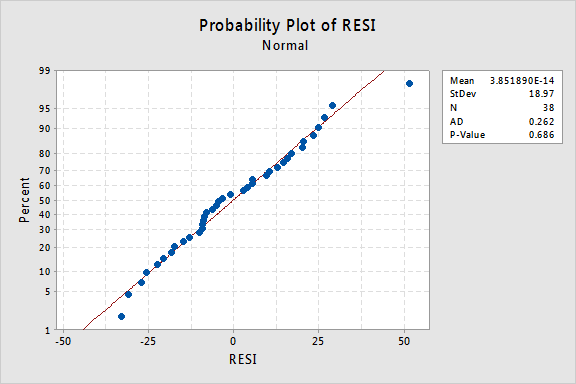
\includegraphics[width=\linewidth]{shapiro.png}
    \caption{Gráfico representando amostra normal segundo o teste de \textit{Kolmogorov-Smirnov} \cite{pensu2017}}
    \label{fig:normalidade}
    \end{figure}

    Da mesma forma, verifica-se se as amostras são homocedásticas. Através do teste de \textit{Levene}, observou-se o \textit{p-value} e foram avalaidas duas hipóteses:

    \begin{itemize}
      \item H0 (hipótese nula): as amostras homocedásticas.
      \item H1 (hipótese alternativa): as amostras não são homocedásticas;
    \end{itemize}

    Ao verificar resultado maior que a significância estabelecida de 5\%, aceita-se a hipótese de que os dados são homocedásticos. É o caso da amostra representada pela figura~\ref{fig:homocedasticidade}

    \begin{figure}[H]
    \centering
      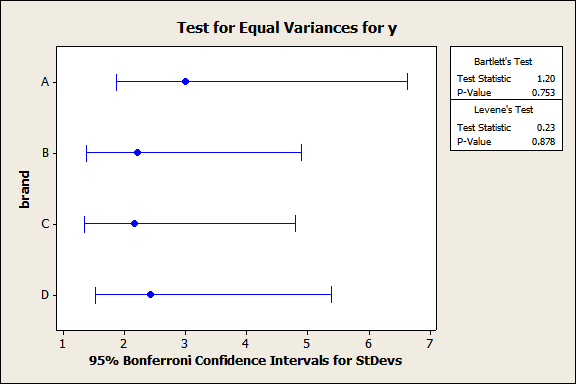
\includegraphics[width=\linewidth]{levene.png}
    \caption{Teste de \textit{Levene} apontando amostra homocedástica \cite{wang2009}}
    \label{fig:homocedasticidade}
    \end{figure}


    Ao garantir que as amostras são normais e homocedásticas, pode-se aplicar um teste paramétrico para verificar se as médias das amostras antes e depois do \textit{code review} são significativamente distintas, do ponto de vista estatístico. Elegeu-se o \textit{Teste T} com os fatores ``antes'' (ACR) e ``depois'' (DCR) da aplicação do \textit{code review}. São as hipóteses:

    \begin{itemize}
      \item H0 (hipótese nula): não há diferença entre as médias;
      \item H1 (hipótese alternativa): há diferença entre as médias.
    \end{itemize}

    Um \textit{p-value} maior que 0,05 indica que deve-se descartar a hipótese nula, como é exemplificado na figura~\ref{fig:test_t}. Caso os dados não sejam normais e homocedásticos, aplica-se testes não paramétricos para chegar a esta conclusão. Para estas situações aplica-se o teste de \textit{Mann-Whitney}, o que pode ser visto na figura~\ref{fig:mannwhitney}.

    \begin{figure}[H]
    \centering
      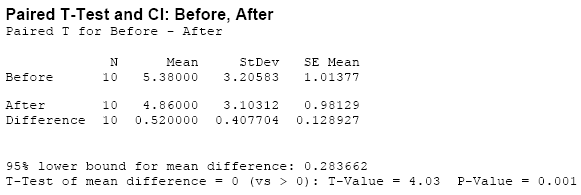
\includegraphics[width=\linewidth]{testt.png}
    \caption{\textit{Teste T} para asserção da significância estatística da amostra \cite{pensu2017b}}
    \label{fig:test_t}
    \end{figure}

    \begin{figure}[H]
    \centering
      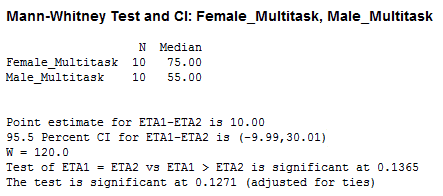
\includegraphics[width=\linewidth]{mann_whitney.png}
    \caption{Teste de \textit{Mann-Whitney} para asserção da significância estatística da amostra \cite{frost2013}}
    \label{fig:mannwhitney}
    \end{figure}


  \section{Execução}

  Para evitar enviesamento das análises, os conjuntos de teste e treinamento da rede são diferentes. Os dados utilizados para montagem da rede variam entre 01/01/2010  e 31/12/2017. Já o conjunto para avaliação está contido entre 01/01/2018 e 31/12/2018. A funcionalidade de avaliação dos resultados salva todas as métricas para cada revisão em cada projeto em arquivos .csv, facilitando análises exploratórias. Dois tipos de avaliação distintos são executadas: para as métricas de proximidade, a comparação é feita entre as três abordagens, agrupados dois a dois. Para as métricas de eficiência a comparação é feita entre os grupos recomendados ($r$) e não recomendados ($w$), para cada método. Em ambos os casos, o valor de $k \in \{1, 3, 5, 10\}$  As figuras mostram, respectivamente, exemplos das saídas para avaliações do primeiro e do segundo grupo.


  \begin{figure}[!htbp]
      \centering
      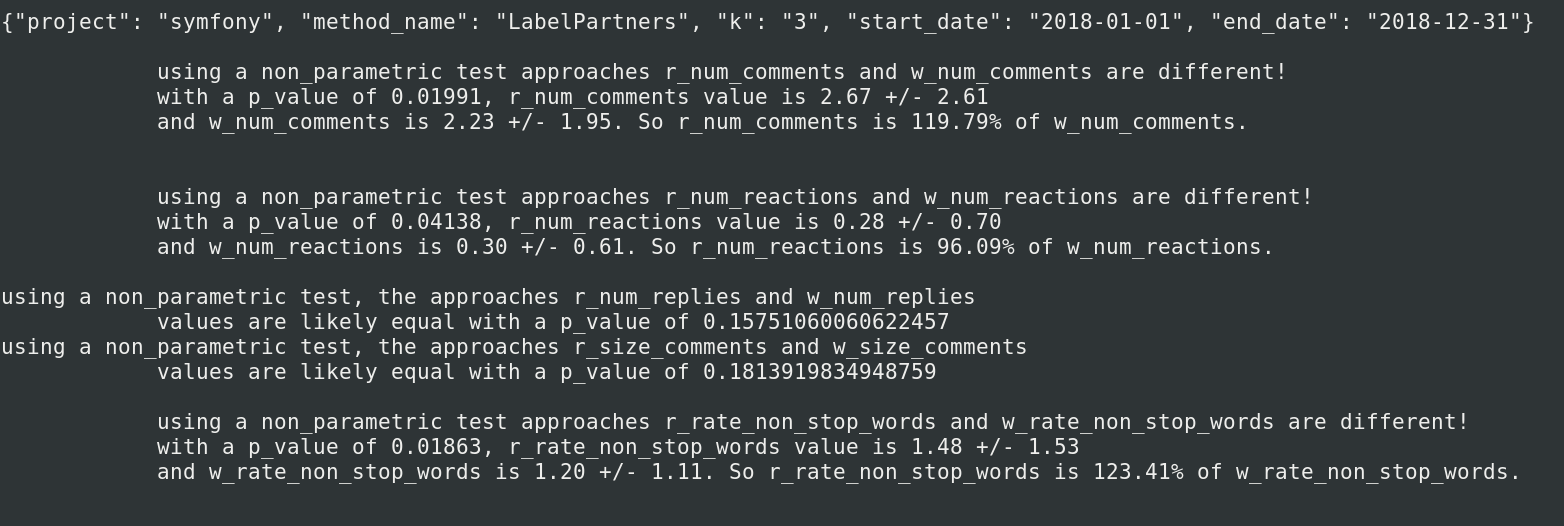
\includegraphics[width=\textwidth]{method-evaluation}
      \caption{Avaliação de Precision no Node.js}\label{fig:method-evaluation}
  \end{figure}


  \begin{figure}[!htbp]
      \centering
      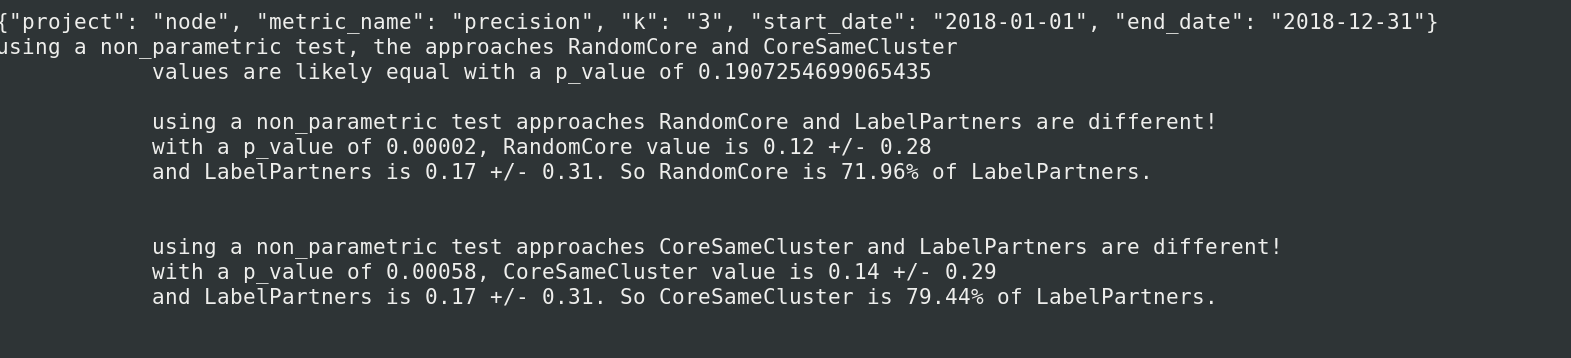
\includegraphics[width=\textwidth]{metric-evaluation}
      \caption{Avaliação das métricas de eficiência do método LabelPartners no Symfony}\label{fig:metric-evaluation}
  \end{figure}

  \section{Apresentação dos resultados}\label{sec:apresentacao}
  A apresentação dos resultados é dividia em duas partes: nas métricas de proximidade e nas métricas de eficiência. Em cada uma delas há a apresentação dos dados brutos e a comparação entre os grupos de análise levando em consideração a significância estatísticas das saídas.

  \subsection{Métricas de Proximidade}

  As métricas de proximidade foram extraídas para cada projeto separadamente. Os resultados Para o projeto Node.js estão nas tabelas~\ref{tab:precision-node} e~\ref{tab:hit-node}. A precisão para $k \in \{1, 3\}$ mostram o método \textit{LabelPartners} ligeiramente melhor, mas com a perda relativa para conjuntos de revisõs maiores. O mesmo acontece com o \textit{hit}, apesar das diferenças para todos valores de $k$ terem sido maiores.

  \begin{table}[htbp]
  \caption{Resultados da Precisão para o Node.js}
  \begin{center}
  \begin{tabular}{|c|c|c|c|}
  \hline
  \textbf{} & \textbf{RandomCore} & \textbf{CoreSameCluster}& \textbf{LabelPartners} \\
  \hline
    1  & 4\%     & 4\%          & 6\%        \\
    3  & 12\%    & 14\%         & 17\%       \\
    5  & 21\%    & 21\%         & 23\%       \\
    10 & 42\%    & 41\%         & 32\%       \\
  \hline
  \end{tabular}
  \label{tab:precision-node}
  \end{center}
  \end{table}


  \begin{table}[htbp]
  \caption{Resultados do \textit{hit} para o Node.js}
  \begin{center}
  \begin{tabular}{|c|c|c|c|}
  \hline
  \textbf{} & \textbf{RandomCore} & \textbf{CoreSameCluster}& \textbf{LabelPartners} \\
  \hline
  1   & 9\%     & 9\%          & 13\%       \\
  3   & 22\%    & 23\%         & 30\%       \\
  5   & 36\%    & 37\%         & 37\%       \\
  10  & 61\%    & 59\%         & 46\%       \\
  \hline
  \end{tabular}
  \label{tab:hit-node}
  \end{center}
  \end{table}

Os resultados das métricas de proximidade para o Symfony foram melhores, para todos os métodos. Os resultados de \textit{hit} apresentados na tabela~\ref{tab:hit-symfony} mostram uma eficiência em até 81\% dos casos. Os resultados de precisão na tabela~\ref{tab:precision-symfony} mostram maior discrepância entre os valores mais baixos de $k$ com o \textit{LabelPartners} em vantagem substancial. O desempenho dos métodos \textit{RandomCore} e \textit{CoreSameCluster} foi similar em todos os casos estudados, superiores ou próximos ao terceiro método para $k$s mais altos.

  \begin{table}[htbp]
  \caption{Resultados da Precisão para o Symfony}
  \begin{center}
  \begin{tabular}{|c|c|c|c|}
  \hline
  \textbf{} & \textbf{RandomCore} & \textbf{CoreSameCluster}& \textbf{LabelPartners} \\
  \hline
    1  & 8\%        & 9\%             & 23\%          \\
    3  & 21\%       & 21\%            & 40\%          \\
    5  & 33\%       & 35\%            & 50\%          \\
    10 & 65\%       & 59\%            & 62\%         \\
  \hline
  \end{tabular}
  \label{tab:precision-symfony}
  \end{center}
  \end{table}


  \begin{table}[htbp]
  \caption{Resultados da \textit{hit} para o Symfony}
  \begin{center}
  \begin{tabular}{|c|c|c|c|}
  \hline
  \textbf{} & \textbf{RandomCore} & \textbf{CoreSameCluster}& \textbf{LabelPartners} \\
  \hline
  1  & 14\%       & 17\%            & 39\%          \\
  3  & 35\%       & 37\%            & 59\%          \\
  5  & 53\%       & 55\%            & 67\%          \\
  10 & 81\%       & 78\%            & 76\%      \\
  \hline
  \end{tabular}
  \label{tab:hit-symfony}
  \end{center}
  \end{table}

No projeto Kubernetes é possível ver maior diferença entre os métodos \textit{RandomCore} e \textit{CoreSameCluster} para as médias da precisão (tabela~\ref{tab:precision-kubernetes}) e \textit{hit}(tabela~\ref{tab:hit-kubernetes}). É também o único caso da superioridade do \textit{LabelPartners} para $k \in \{5, 10\}$

  \begin{table}[htbp]
  \caption{Resultados da Precisão para o Kubernetes}
  \begin{center}
  \begin{tabular}{|c|c|c|c|}
  \hline
  \textbf{} & \textbf{RandomCore} & \textbf{CoreSameCluster}& \textbf{LabelPartners} \\
  \hline
  1  & 2\%        & 5\%             & 11\%          \\
  3  & 6\%        & 8\%             & 21\%          \\
  5  & 9\%        & 13\%            & 26\%          \\
  10 & 18\%       & 21\%            & 32\%          \\
  \hline
  \end{tabular}
  \label{tab:precision-kubernetes}
  \end{center}
  \end{table}


  \begin{table}[htbp]
  \caption{Resultados da \textit{hit} para o Kubernetes}
  \begin{center}
  \begin{tabular}{|c|c|c|c|}
  \hline
  \textbf{} & \textbf{RandomCore} & \textbf{CoreSameCluster}& \textbf{LabelPartners} \\
  \hline
  1  & 3\%        & 7\%             & 18\%          \\
  3  & 10\%       & 14\%            & 21\%          \\
  5  & 14\%       & 20\%            & 37\%          \\
  10 & 28\%       & 31\%            & 42\%          \\
  \hline
  \end{tabular}
  \label{tab:hit-kubernetes}
  \end{center}
  \end{table}

  Os resultados da precisão (tabela~\ref{tab:precision-tensorflow}) e \textit{hit} (tabela~\ref{tab:hit-tensorflow}) do projeto Tensorflow mostram superioridade leve do \textit{LabelPartners}, além de uma diferença maior entre os métodos \textit{RandomCore} e \textit{CoreSameCluster}, com o segundo sendo mais eficiente para valores de $k$ mais baixos.


  \begin{table}[htbp]
  \caption{Resultados da Precisão para o Tensorflow}
  \begin{center}
  \begin{tabular}{|c|c|c|c|}
  \hline
  \textbf{} & \textbf{RandomCore} & \textbf{CoreSameCluster}& \textbf{LabelPartners} \\
  \hline
  1  & 2\%        & 4\%             & 9\%           \\
  3  & 11\%       & 12\%            & 15\%          \\
  5  & 16\%       & 18\%            & 27\%          \\
  10 & 35\%       & 35\%            & 42\%          \\
  \hline
  \end{tabular}
  \label{tab:precision-tensorflow}
  \end{center}
  \end{table}

  \begin{table}[htbp]
  \caption{Resultados da \textit{hit} para o Tensorflow}
  \begin{center}
  \begin{tabular}{|c|c|c|c|}
  \hline
  \textbf{} & \textbf{RandomCore} & \textbf{CoreSameCluster}& \textbf{LabelPartners} \\
  \hline
    1  & 2\%        & 4\%             & 10\%          \\
    3  & 13\%       & 13\%            & 16\%          \\
    5  & 18\%       & 21\%            & 29\%          \\
    10 & 38\%       & 39\%            & 46\%          \\
  \hline
  \end{tabular}
  \label{tab:hit-tensorflow}
  \end{center}
  \end{table}


Apesar de um domínio aparente do \textit{LabelPartners} para valores de $k$ mais baixos, outro comportamento pode ser observado nas figuras~\ref{fig:perf-precision} e~\ref{fig:perf-hit}, que comparam a precisão e o \textit{hit} dos métodos. Em dois casos a eficiência para $k$ mais altos fica próxima para todos os métodos, enquanto em dois outros casos se observa uma escalabilidade maior dos métodos baseados em \textit{cores}, linear, enquanto o \textit{LabelPartners} não acompanha a mesma tendência. A aproximação dos métodos se dá em conjuntos de recomendações maiores pois quando não há mais \textit{cores} do mesmo grupo ou parceiros de revisão suficientes para indicação, todos os métodos recorrem a lista completa de \textit{cores} do repositório. Assim a tendência é que para $k$s mais altos o grupo recomendado seja muito parecido, levando ao resultado próximo. Além disso, como  grande parte das revisões possui apenas um revisor (como mostrado na figura~\ref{fig:dist-rc}), o valor das duas métricas tende a ficar mais próximo.


  \begin{figure}[htbp]
     \centering
     \begin{subfigure}[b]{0.475\textwidth}
         \centering
         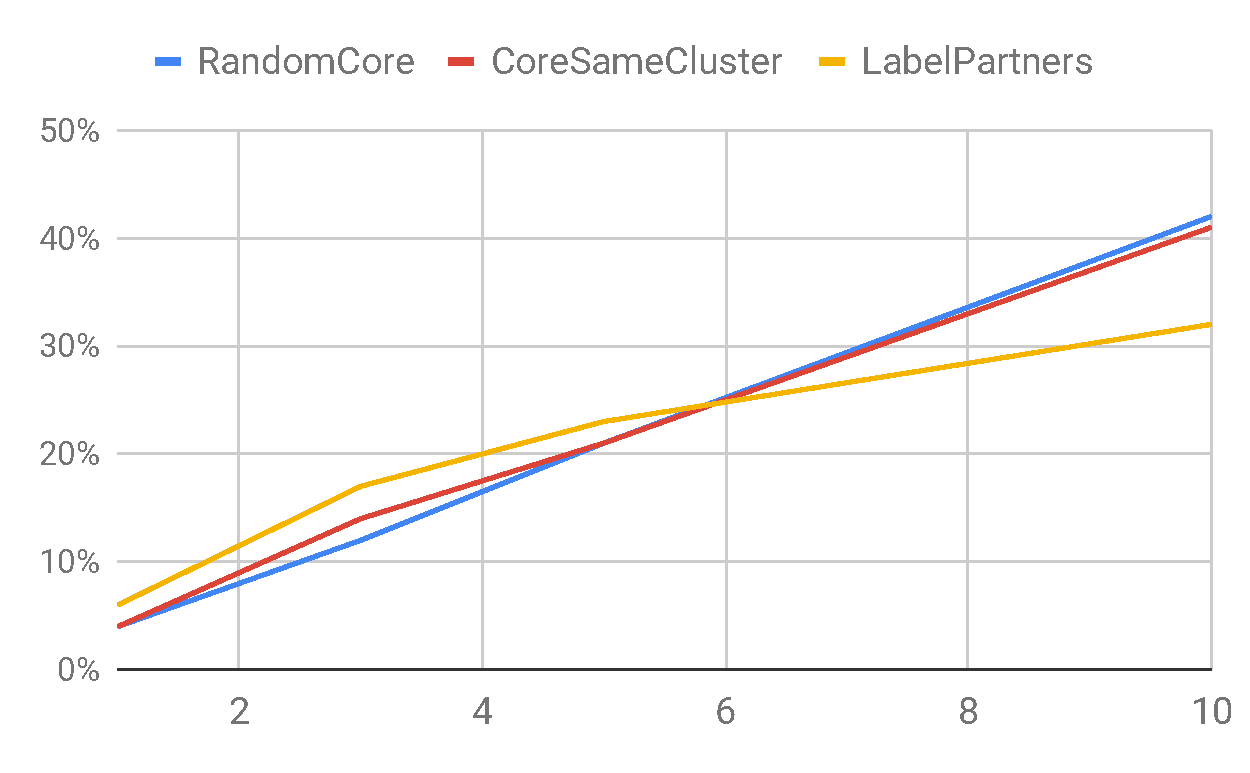
\includegraphics[width=\textwidth]{resultados/perf-precision-node}
         \caption[Node.js]%
         {{\small Node.js}}
         \label{fig:perf-precision-node}
     \end{subfigure}
     \hfill
     \begin{subfigure}[b]{0.475\textwidth}
         \centering
         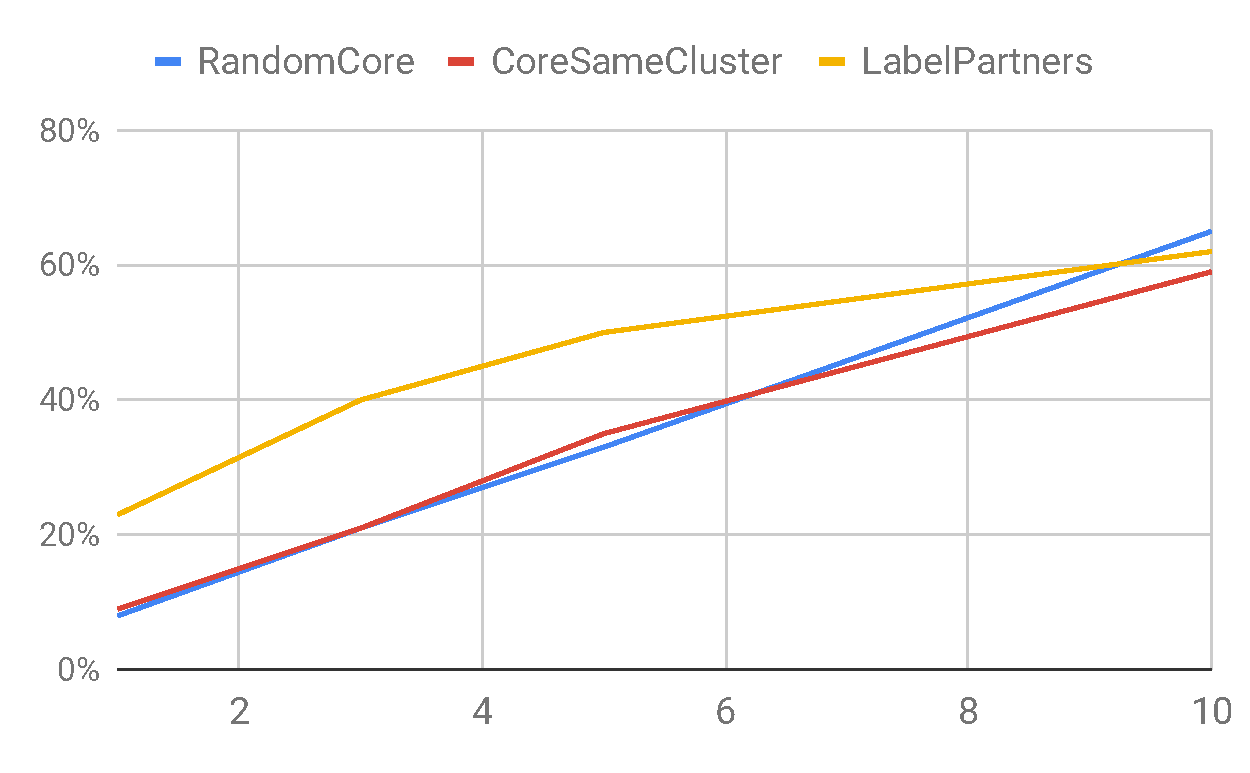
\includegraphics[width=\textwidth]{resultados/perf-precision-symfony}
         \caption[Symfony]%
         {{\small Symfony}}
         \label{fig:perf-precision-symfony}
     \end{subfigure}
     \vskip\baselineskip
     \begin{subfigure}[b]{0.475\textwidth}
         \centering
         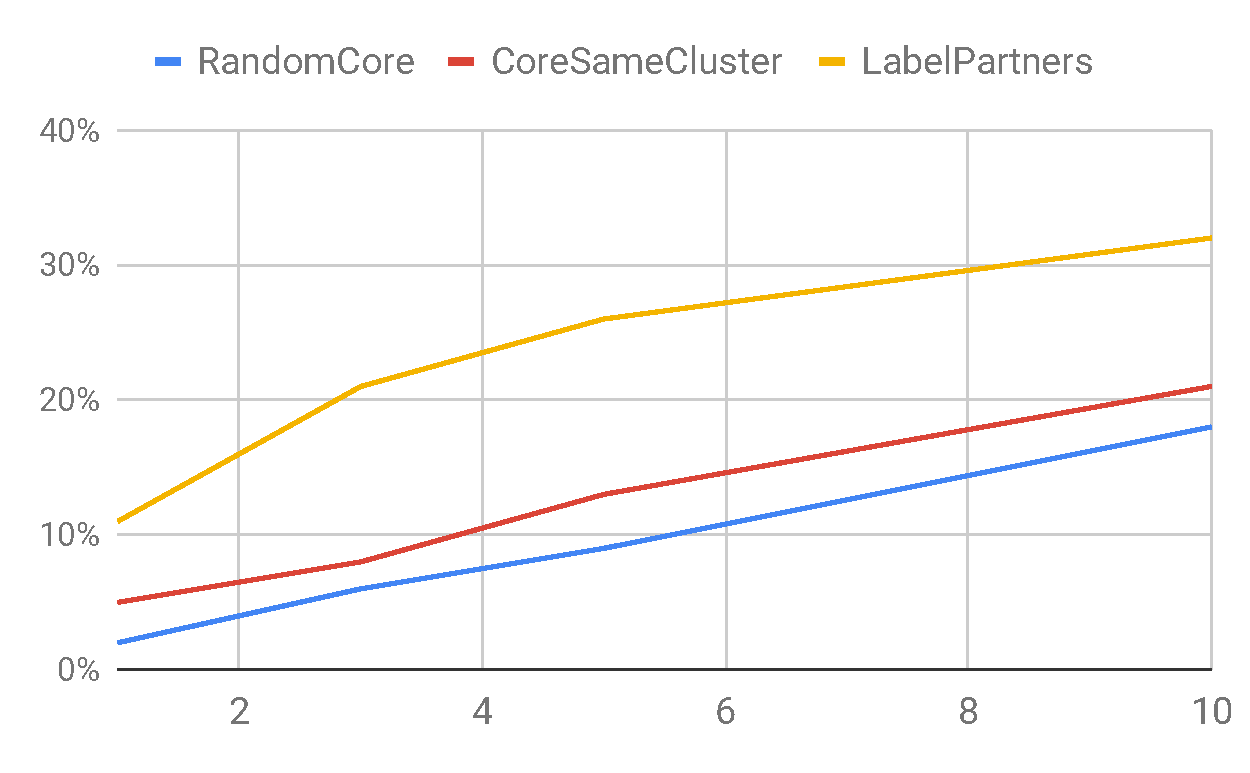
\includegraphics[width=\textwidth]{resultados/perf-precision-kubernetes}

         \caption[Kubernetes]%
         {{\small Kubernetes}}
         \label{fig:perf-precision-kubernetes}
     \end{subfigure}
     \quad
     \begin{subfigure}[b]{0.475\textwidth}
         \centering
         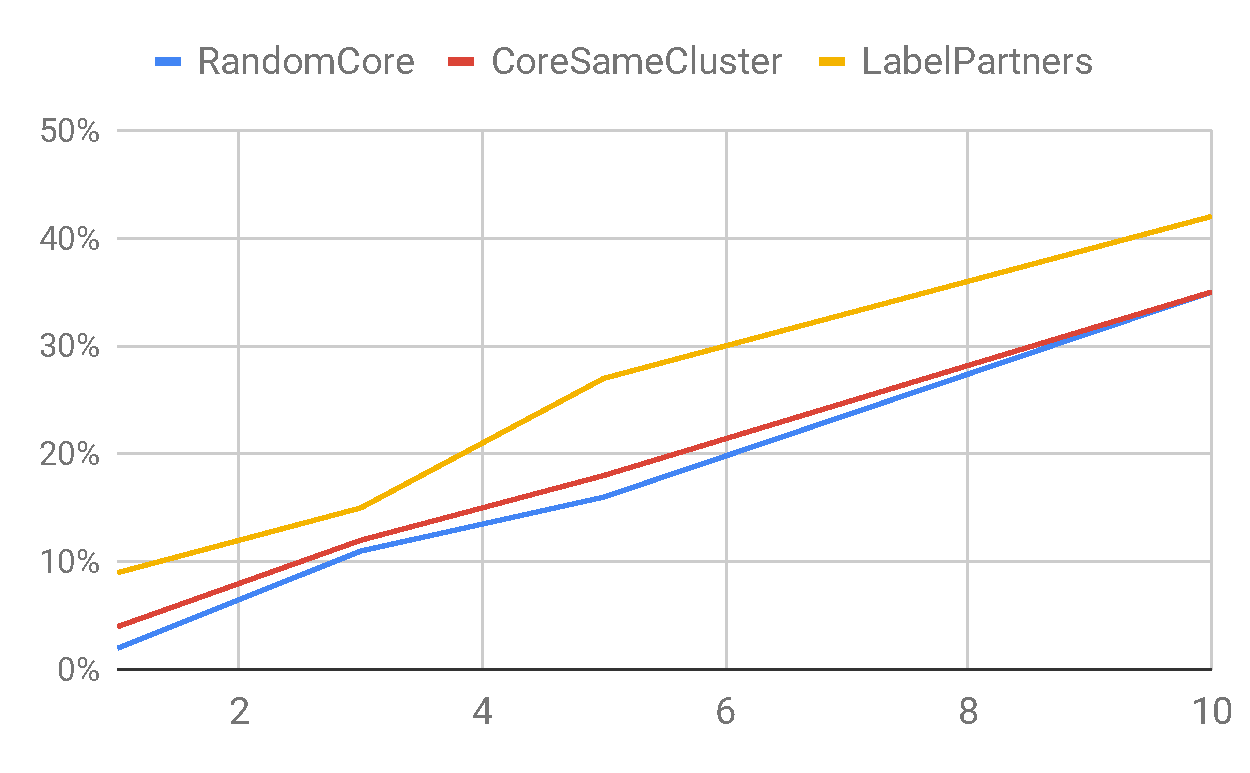
\includegraphics[width=\textwidth]{resultados/perf-precision-tensorflow}
         \caption[Tensorflow]%
         {{\small Tensorflow}}
         \label{fig:perf-precision-tensorflow}
     \end{subfigure}
     \caption[]
     {\small Comparação da precisão entre os diferentes métodos.}
     \label{fig:perf-precision}
 \end{figure}

O maior desempenho dos algoritmos 1 e 2 para $k$s elevados pode ser justificada pela quantidade indicação de indivíduos centrais no projeto, que tem a responsabilidade (e nível de permissão) para aceitar o \textit{``pull request''}. Apesar de potencializar os resultados nas métricas de proximidade, ainda é preciso avaliar se estes indivíduos tem a disponibilidade e as habilidades interpessoais para realizar boas revisões, segundo as métricas de eficiência escolhidas.



  \begin{figure}[htbp]
     \centering
     \begin{subfigure}[b]{0.475\textwidth}
         \centering
         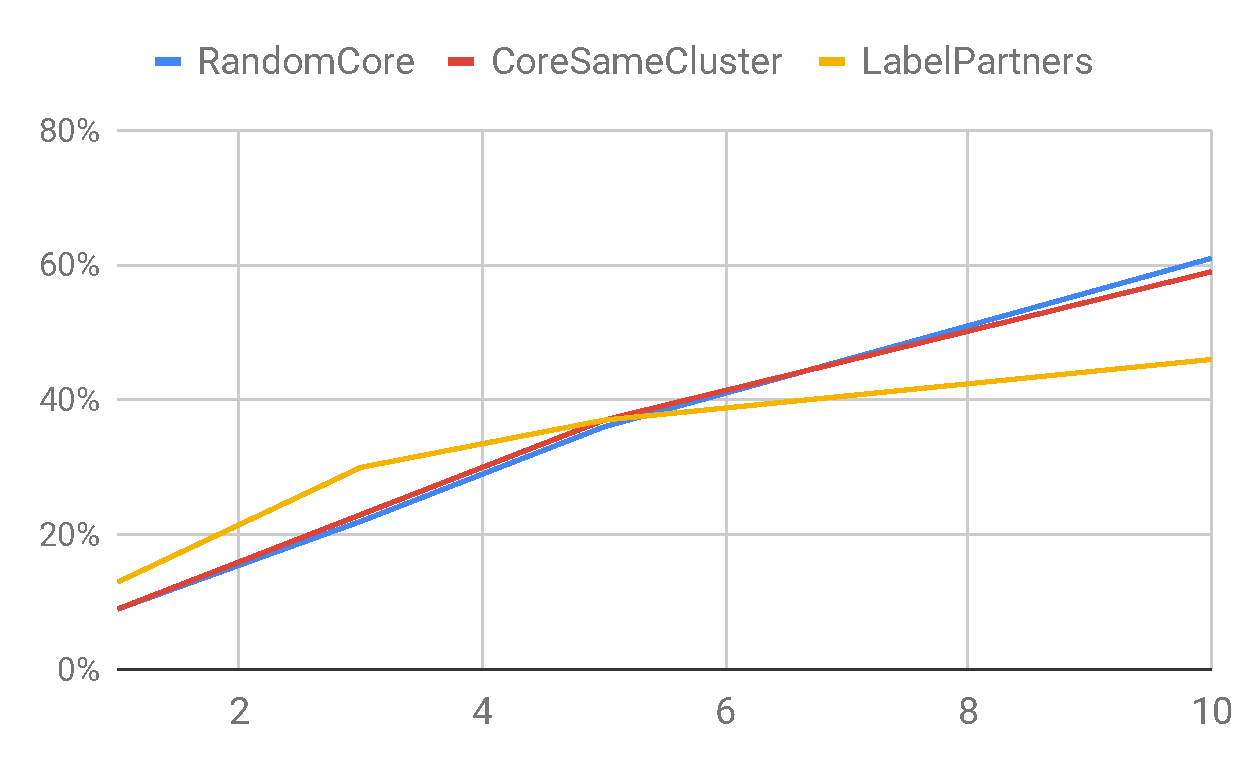
\includegraphics[width=\textwidth]{resultados/perf-hit-node}
         \caption[Node.js]%
         {{\small Node.js}}
         \label{fig:perf-hit-node}
     \end{subfigure}
     \hfill
     \begin{subfigure}[b]{0.475\textwidth}
         \centering
         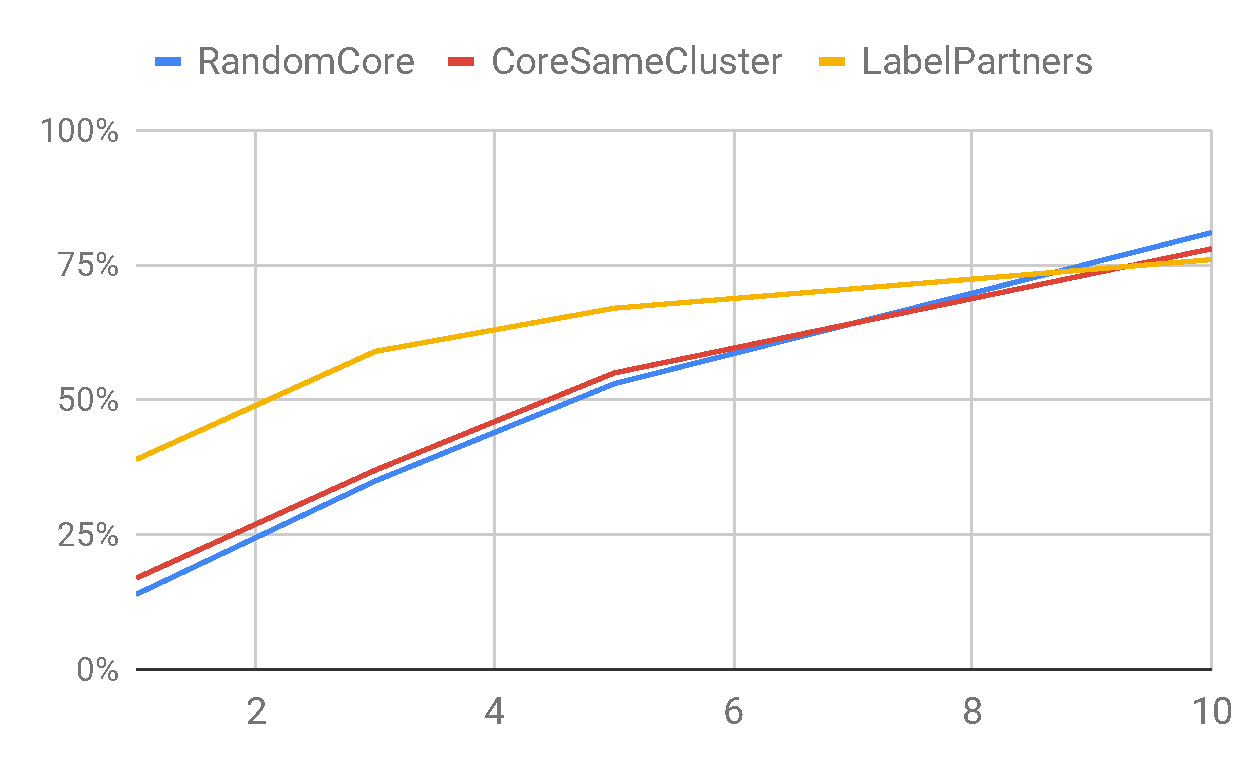
\includegraphics[width=\textwidth]{resultados/perf-hit-symfony}
         \caption[Symfony]%
         {{\small Symfony}}
         \label{fig:perf-hit-symfony}
     \end{subfigure}
     \vskip\baselineskip
     \begin{subfigure}[b]{0.475\textwidth}
         \centering
         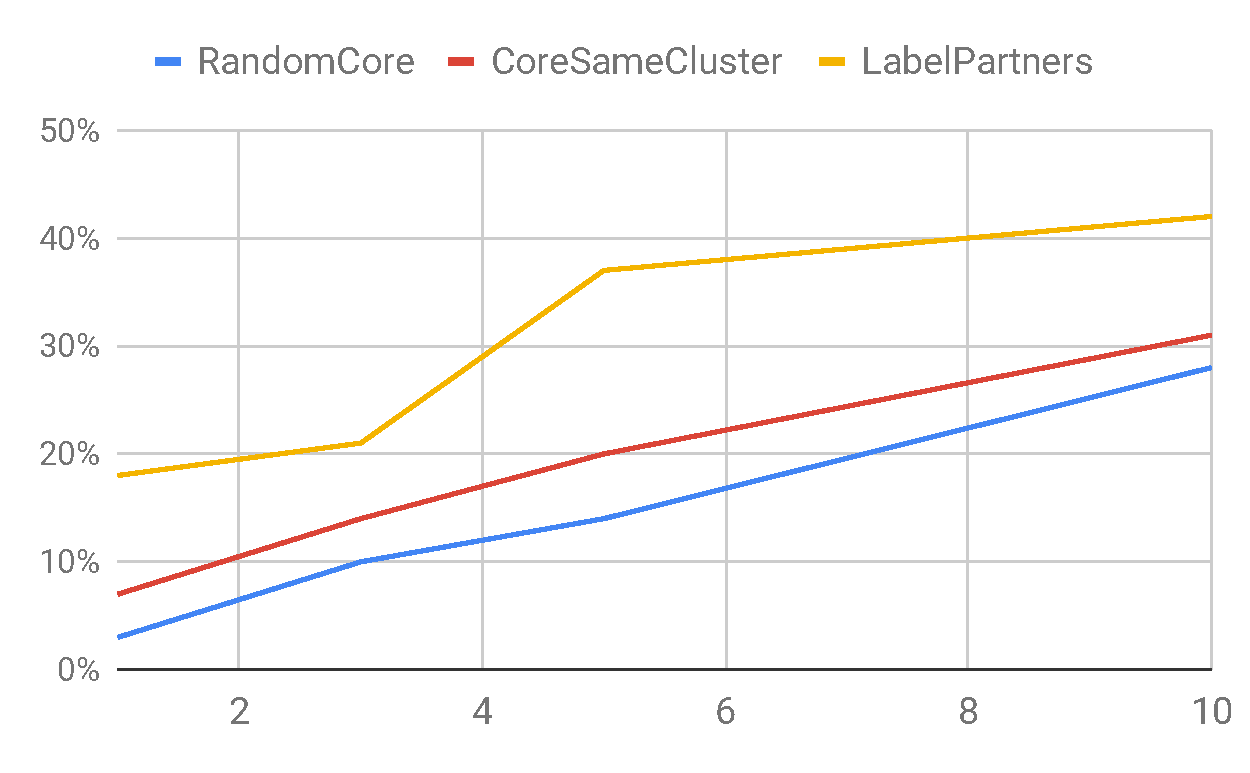
\includegraphics[width=\textwidth]{resultados/perf-hit-kubernetes}

         \caption[Kubernetes]%
         {{\small Kubernetes}}
         \label{fig:perf-hit-kubernetes}
     \end{subfigure}
     \quad
     \begin{subfigure}[b]{0.475\textwidth}
         \centering
         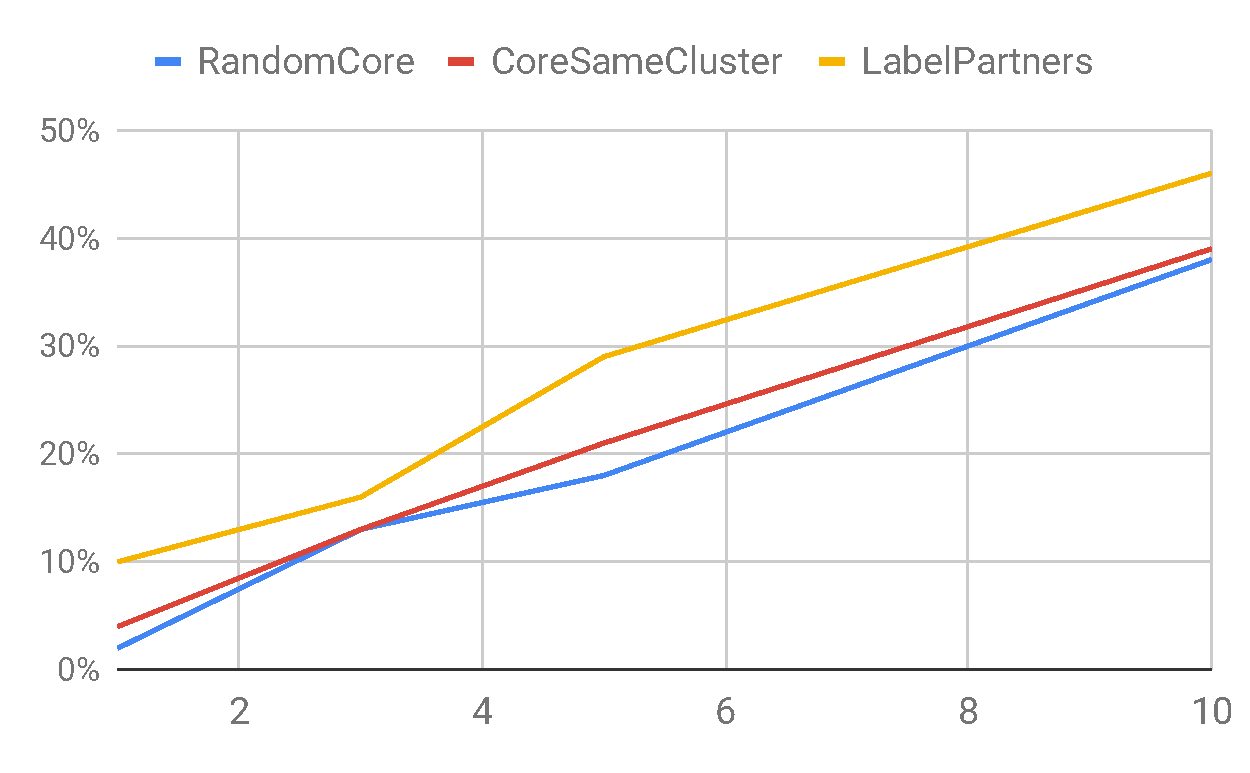
\includegraphics[width=\textwidth]{resultados/perf-hit-tensorflow}
         \caption[Tensorflow]%
         {{\small Tensorflow}}
         \label{fig:perf-hit-tensorflow}
     \end{subfigure}
     \caption[]
     {\small Comparação da precisão entre os diferentes métodos.}
     \label{fig:perf-hit}
 \end{figure}

 Apesar da análise visual dos comportamentos dos métodos perante a variação do conjunto recomendado, é necessário avaliar em quais casos houve diferença significativa entre as performances observadas. Como explicado na seção~\ref{sec:significancia}, os métodos são comparados dois a dois. São definidas as seguintes hipóteses para a precisão:

 \begin{itemize}
   \item H0 (hipótese nula): os métodos possuem precisão igual;
   \item H1 (hipótese alternativa): os métodos possuem precisões diferentes.
 \end{itemize}

 Já para o \textit{hit} as seguintes hipóteses são levantadas:

  \begin{itemize}
    \item H0 (hipótese nula): os métodos possuem desempenho igual;
    \item H1 (hipótese alternativa): os métodos possuem desempenho distinto.
  \end{itemize}

 As amostras com resultados dos testes paramétricos ou não paramétricos executados (de acordo com o protocolo apresentado na seção~\ref{sec:significancia}) onde $ p < 0.05 $ são considerados estatisticamente relevantes, e apresentados na tabelas~\ref{tab:resultados-precisao} e~\ref{tab:resultados-hit}.

 \begin{table}[htbp]
 \caption{Comparação da precisão apontando para diferenças estatisticamente relevantes}
 \begin{center}
   \resizebox{\textwidth}{!}{%
   \begin{tabular}{|c|c|c|c|c|c|c|c|c|}
     \hline
   \textbf{Projeto} & \textbf{k} & \textbf{Método A} & \textbf{Método B} & \textbf{Média A} & \textbf{Média B} & \textbf{Tipo de Teste} & \textbf{p-value} & \textbf{Proporção} \\
   \hline

   Node.js          & 1          & RandomCore        & LabelPartners     & 0.04             & 0.06              & Não Paramétrico        & 0.006            & 72\%               \\
   Node.js          & 1          & CoreSameCluster   & LabelPartners     & 0.04             & 0.06              & Não Paramétrico        & 0.001            & 72\%               \\
   Node.js          & 3          & RandomCore        & LabelPartners     & 0.12             & 0.17             & Não Paramétrico        & 0.00002          & 71\%               \\
   Node.js          & 3          & CoreSameCluster   & LabelPartners     & 0.14             & 0.17             & Não Paramétrico        & 0.00058          & 79\%               \\
   Node.js          & 10         & RandomCore        & LabelPartners     & 0.42             & 0.32             & Não Paramétrico        & 0.00000          & 130\%              \\
   Node.js          & 10         & CoreSameCluster   & LabelPartners     & 0.40             & 0.32             & Não Paramétrico        & 0.00000          & 127\%              \\
   Symfony          & 1          & RandomCore        & LabelPartners     & 0.08             & 0.23             & Não Paramétrico        & 0.00000          & 33\%               \\
   Symfony          & 1          & CoreSameCluster   & LabelPartners     & 0.09             & 0.23             & Não Paramétrico        & 0.00000          & 38\%               \\
   Symfony          & 3          & RandomCore        & LabelPartners     & 0.21             & 0.40             & Não Paramétrico        & 0.00000          & 52\%               \\
   Symfony          & 3          & CoreSameCluster   & LabelPartners     & 0.21             & 0.40             & Não Paramétrico        & 0.00000          & 52\%               \\
   Symfony          & 5          & RandomCore        & LabelPartners     & 0.33             & 0.50             & Não Paramétrico        & 0.00000          & 65\%               \\
   Symfony          & 5          & CoreSameCluster   & LabelPartners     & 0.35             & 0.50             & Não Paramétrico        & 0.00000          & 68\%               \\
   Symfony          & 10         & RandomCore        & CoreSameCluster   & 0.65             & 0.59             & Não Paramétrico        & 0.00826          & 109\%              \\
   Kubernetes       & 1          & RandomCore        & CoreSameCluster   & 0.02             & 0.05             & Não Paramétrico        & 0.00000          & 37\%               \\
   Kubernetes       & 1          & RandomCore        & LabelPartners     & 0.02             & 0.11             & Não Paramétrico        & 0.00000          & 15\%               \\
   Kubernetes       & 1          & CoreSameCluster   & LabelPartners     & 0.05             & 0.11             & Não Paramétrico        & 0.00000          & 40\%               \\
   Kubernetes       & 3          & RandomCore        & CoreSameCluster   & 0.06             & 0.08             & Não Paramétrico        & 0.00004          & 69\%               \\
   Kubernetes       & 3          & RandomCore        & LabelPartners     & 0.06             & 0.35             & Não Paramétrico        & 0.00000          & 27\%               \\
   Kubernetes       & 3          & CoreSameCluster   & LabelPartners     & 0.08             & 0.35             & Não Paramétrico        & 0.00000          & 39\%               \\
   Kubernetes       & 5          & RandomCore        & CoreSameCluster   & 0.09             & 0.13             & Não Paramétrico        & 0.00000          & 70\%               \\
   Kubernetes       & 5          & RandomCore        & LabelPartners     & 0.09             & 0.26             & Não Paramétrico        & 0.00000          & 34\%               \\
   Kubernetes       & 5          & CoreSameCluster   & LabelPartners     & 0.13             & 0.26             & Não Paramétrico        & 0.00000          & 48\%               \\
   Kubernetes       & 10         & RandomCore        & CoreSameCluster   & 0.18             & 0.21             & Não Paramétrico        & 0.00801          & 88\%               \\
   Kubernetes       & 10         & RandomCore        & LabelPartners     & 0.18             & 0.32             & Não Paramétrico        & 0.00000          & 56\%               \\
   Kubernetes       & 10         & CoreSameCluster   & LabelPartners     & 0.21             & 0.32             & Não Paramétrico        & 0.00000          & 64\%               \\
   Tensorflow       & 1          & RandomCore        & CoreSameCluster   & 0.02             & 0.04             & Não Paramétrico        & 0.02871          & 41\%               \\
   Tensorflow       & 1          & RandomCore        & LabelPartners     & 0.02             & 0.09             & Não Paramétrico        & 0.00000          & 18\%               \\
   Tensorflow       & 1          & CoreSameCluster   & LabelPartners     & 0.04             & 0.09             & Não Paramétrico        & 0.00286          & 44\%               \\
   Tensorflow       & 5          & RandomCore        & LabelPartners     & 0.16             & 0.27             & Não Paramétrico        & 0.00020          & 33\%               \\
   Tensorflow       & 5          & CoreSameCluster   & LabelPartners     & 0.18             & 0.27             & Não Paramétrico        & 0.00261          & 38\%               \\
   Tensorflow       & 10         & RandomCore        & LabelPartners     & 0.35             & 0.42             & Não Paramétrico        & 0.01961          & 83\%               \\
   Tensorflow       & 10         & CoreSameCluster   & LabelPartners     & 0.35             & 0.42             & Não Paramétrico        & 0.02402          & 83\%               \\
   \end{tabular}%
   }
   \hline

 \label{tab:resultados-precisao}
 \end{center}
 \end{table}


 É possível observar que em todos os casos as amostras não eram homocedásticas e normais, e por isso foram aplicados testes não paramêtricos. Foram poucos os casos onde existiu diferença significativa entre os métodos \textit{RandomCore} e \textit{CoreSameCluster}, notoriamente no projeto Kubernetes. A maior parte das comparações significativas mostra o método \textit{LabelPartners} como mais preciso, salvo em casos de $k = 10$ no Node.js.


 \begin{table}[htbp]
 \caption{Comparação do \textit{hit} apontando para diferenças estatisticamente relevantes}
 \begin{center}
   \resizebox{\textwidth}{!}{%
   \begin{tabular}{|c|c|c|c|c|c|c|c|c|}
     \hline
   \textbf{Projeto} & \textbf{k} & \textbf{Método A} & \textbf{Método B} & \textbf{Média A} & \textbf{Média B} & \textbf{Tipo de Teste} & \textbf{p-value} & \textbf{Proporção} \\
\hline
   Node.js          & 1          & RandomCore        & LabelPartners     & 0.09             & 0.13             & Não Paramétrico        & 0.00572          & 72\%               \\
   Node.js          & 1          & CoreSameCluster   & LabelPartners     & 0.9              & 0.13             & Não Paramétrico        & 0.00175          & 68\%               \\
   Node.js          & 3          & RandomCore        & LabelPartners     & 0.22             & 0.30             & Não Paramétrico        & 0.0002           & 72\%               \\
   Node.js          & 3          & CoreSameCluster   & LabelPartners     & 0.23             & 0.30             & Não Paramétrico        & 0.0037           & 77\%               \\
   Node.js          & 10         & RandomCore        & LabelPartners     & 0.61             & 0.46             & Não Paramétrico        & 0.00000          & 133\%              \\
   Node.js          & 10         & CoreSameCluster   & LabelPartners     & 0.59             & 0.46             & Não Paramétrico        & 0.00000          & 129\%              \\
   Symfony          & 1          & RandomCore        & LabelPartners     & 0.14             & 0.39             & Não Paramétrico        & 0.00000          & 34\%               \\
   Symfony          & 1          & CoreSameCluster   & LabelPartners     & 0.17             & 0.39             & Não Paramétrico        & 0.00000          & 42\%               \\
   Symfony          & 3          & RandomCore        & LabelPartners     & 0.35             & 0.49             & Não Paramétrico        & 0.00000          & 59\%               \\
   Symfony          & 3          & CoreSameCluster   & LabelPartners     & 0.37             & 0.49             & Não Paramétrico        & 0.00000          & 62\%               \\
   Symfony          & 5          & RandomCore        & LabelPartners     & 0.53             & 0.67             & Não Paramétrico        & 0.00000          & 79\%               \\
   Symfony          & 5          & CoreSameCluster   & LabelPartners     & 0.55             & 0.67             & Não Paramétrico        & 0.00002          & 82\%               \\
   Symfony          & 10         & RandomCore        & LabelPartners     & 0.81             & 0.79             & Não Paramétrico        & 0.01013          & 107\%              \\
   Kubernetes       & 1          & RandomCore        & CoreSameCluster   & 0.03             & 0.07             & Não Paramétrico        & 0.00000          & 39\%               \\
   Kubernetes       & 1          & RandomCore        & LabelPartners     & 0.03             & 0.18             & Não Paramétrico        & 0.00000          & 15\%               \\
   Kubernetes       & 1          & CoreSameCluster   & LabelPartners     & 0.07             & 0.18             & Não Paramétrico        & 0.00000          & 39\%               \\
   Kubernetes       & 3          & RandomCore        & CoreSameCluster   & 0.10             & 0.14             & Não Paramétrico        & 0.00005          & 73\%               \\
   Kubernetes       & 3          & RandomCore        & LabelPartners     & 0.10             & 0.31             & Não Paramétrico        & 0.00000          & 32\%               \\
   Kubernetes       & 3          & CoreSameCluster   & LabelPartners     & 0.14             & 0.31             & Não Paramétrico        & 0.00000          & 43\%               \\
   Kubernetes       & 5          & RandomCore        & CoreSameCluster   & 0.14             & 0.20             & Não Paramétrico        & 0.00000          & 72\%               \\
   Kubernetes       & 5          & RandomCore        & LabelPartners     & 0.14             & 0.37             & Não Paramétrico        & 0.00000          & 39\%               \\
   Kubernetes       & 5          & CoreSameCluster   & LabelPartners     & 0.20             & 0.37             & Não Paramétrico        & 0.00000          & 54\%               \\
   Kubernetes       & 10         & RandomCore        & CoreSameCluster   & 0.28             & 0.31             & Não Paramétrico        & 0.01013          & 89\%               \\
   Kubernetes       & 10         & RandomCore        & LabelPartners     & 0.28             & 0.42             & Não Paramétrico        & 0.00000          & 65\%               \\
   Kubernetes       & 10         & CoreSameCluster   & LabelPartners     & 0.31             & 0.42             & Não Paramétrico        & 0.00000          & 72\%               \\
   Tensorflow       & 1          & RandomCore        & CoreSameCluster   & 0.02             & 0.04             & Não Paramétrico        & 0.02834          & 43\%               \\
   Tensorflow       & 1          & RandomCore        & LabelPartners     & 0.02             & 0.10             & Não Paramétrico        & 0.00000          & 20\%               \\
   Tensorflow       & 1          & CoreSameCluster   & LabelPartners     & 0.04             & 0.10             & Não Paramétrico        & 0.00290          & 45\%               \\
   Tensorflow       & 5          & RandomCore        & LabelPartners     & 0.18             & 0.29             & Não Paramétrico        & 0.00022          & 61\%               \\
   Tensorflow       & 5          & CoreSameCluster   & LabelPartners     & 0.21             & 0.29             & Não Paramétrico        & 0.00283          & 69\%               \\
   Tensorflow       & 10         & RandomCore        & LabelPartners     & 0.38             & 0.46             & Não Paramétrico        & 0.02034          & 83\%               \\
   Tensorflow       & 10         & CoreSameCluster   & LabelPartners     & 0.39             & 0.46             & Não Paramétrico        & 0.02915          & 84\%
   \end{tabular}%
   }
   \hline


 \label{tab:resultados-hit}
 \end{center}
 \end{table}

 O comportamento das medições significativas do \textit{hit} é muito próximo da precisão. Em apenas um dos casos de comparação com $p < 0.05$ (Symfony, $k = 10$) não houve diferença relevante no mesmo caso para ambas as métricas de proximidade.


\subsection{Métricas de eficiência}

As métricas de eficiência se aproximam mais dos objetivos do presente trabalho, uma vez que através delas busca-se traduzir se os métodos apresentados potencializam a colaboração no contexto estudado. Para isso é necessário comparar dois grupos distintos de revisores: aqueles que foram recomendados pelos métodos e aqueles que não foram. A diferença no desempenho destes conjuntos pode indicar em quais casos os métodos são responsáveis por indicar indivíduos aptos à um grau maior de colaboração, interação e convergência com os objetivos da revisão de código no desenvolvimento distribuído, amplamente apresentados e discutidos neste trabalho. Diferente das métricas de proximidade, apenas os resultados significativos serão apresentados aqui, em decorrência do espaço necessário para análise de um grupo maior de métricas. Como descrito anteriormente, é necessário definir a hipótese nula e alternativa para cada métrica. São apresentados os casos onde $p < 0.05$. A tabela~\ref{tab:metricas-eficiencia-hipoteses} descreve as métricas, sua simbologia e as hipóteses referentes a cada uma delas.

\begin{table}[htbp]
\caption{Métricas de proximidade e as respectivas hipóteses }
\begin{center}
  \bgroup
  \def\arraystretch{1.8}%
  \resizebox{\textwidth}{!}{%
  \begin{tabular}{|C|C|C|C|C|}
  \hline
  Métrica                       & Variável               & Descrição                                                                             & H0 (hipótese nula)                                                                               & H1 (hipótese alternativa) \\
  \hline
  Número de Comentários         & $num\_comments$          & \multicolumn{1}{p{5cm}|}{\raggedright Média da quantidade de comentários que cada revisor fez por revisão}                   & \multicolumn{1}{p{7cm}|}{\raggedright Os recomendados pelo método proposto fazem comentários do mesmo tamanho que os não recomendados} & \multicolumn{1}{p{7cm}|}{\raggedright  Os  recomendados pelo método proposto fazem comentários de tamanho distinto em relação aos não recomendados} \\
  Número de Reações             & $num\_reactions$         & \multicolumn{1}{p{5cm}|}{\raggedright Média de reações que cada revisor recebeu por revisão}                                 & \multicolumn{1}{p{7cm}|}{\raggedright Os recomendados pelo método proposto recebem a mesma quantidade de reações que os não recomendados}                      & \multicolumn{1}{p{7cm}|}{\raggedright Os recomendados pelo método proposto recebem quantidades distintas de reações em relação aos não recomendados}                    \\
  Número de repostas            & $num\_replies$           & \multicolumn{1}{p{5cm}|}{\raggedright Média de respostas que cada revisor recebeu por revisão}                               & \multicolumn{1}{p{7cm}|}{\raggedright Os recomendados pelo método proposto recebem a mesma quantidade de respostas que os não recomendados}                    & \multicolumn{1}{p{7cm}|}{\raggedright Os recomendados pelo método proposto recebem quantidades distintas de respostas em relação aos não recomendados}                  \\
  Tamanho dos comentários       & $size\_comments$         & \multicolumn{1}{p{5cm}|}{\raggedright Tamanho médio dos comentários que cada revisor fez por revisão}                        & \multicolumn{1}{p{7cm}|}{\raggedright Os recomendados pelo método proposto escrevem comentários do mesmo tamanho que os não recomendados}                      & \multicolumn{1}{p{7cm}|}{\raggedright Os recomendados pelo método proposto escrevem comentários de tamanho distintinto em relação aos não recomendados}                 \\
  Proporção de \textit{non stop words} & $rate\_non\_stop\_words$ & \multicolumn{1}{p{5cm}|}{\raggedright Média da proporção de \textit{non stop words} dos comentários que cada revisor fez por revisão} & \multicolumn{1}{p{7cm}|}{\raggedrights Os comentários dos recomendados pelo método proposto apresentam a mesma proporção de \textit{non stop words} que os não recomendados} & \multicolumn{1}{p{7cm}|}{\raggedright Os comentários dos recomendados pelo método proposto apresentam proporção de \textit{non stop words} distinta em relação aos não recomendados}
                                                                                               &
  \end{tabular}%\end{tabular}
  }
  \hline
  \egroup
\label{tab:metricas-eficiencia-hipoteses}
\end{center}
\end{table}

A análise é feita para cada um dos projetos, com o tamanho dos grupos recomendados $k \in \{1, 3, 5, 10\}$ já aplicados anteriormente, de forma a facilitar posteriores comparações. Para cada método são executados 80 combinações diferentes de projetos, $k$s e métricas de avaliação. Os resultados são apresentados em tabelas distintas. Para o \textit{RandomCore}, como apresenta a tabela~\ref{tab:resultados-randomcore}, foram poucos os casos testados onde pode ser observada diferença significativa entre os grupos de recomendados e não recomendados. Neles, a maioria expressa uma diferença pequena entre os groupos ou ainda situações onde os indivíduos recomendados se saem pior do que os não recomendados.

\begin{table}[htbp]
\centering
\resizebox{\textwidth}{!}{%
\begin{tabular}{|c|c|c|c|c|c|c|c|}
\hline
\textbf{Projeto} & \textbf{k} & \textbf{Métrica}       & \textbf{Média Recomendados} & \textbf{Média Não Recomendados} & \textbf{Tipo de Teste} & \textbf{p-value} & \textbf{Proporção} \\
\hline
Node.js    & 1  & num\_comments          & 2.39               & 2.36                   & Não Paramétrico & 0.03016 & 101\%     \\
Node.js    & 1  & num\_replies           & 1.20               & 1.34                   & Não Paramétrico & 0.00638 & 90\%      \\
Node.js    & 3  & rate\_non\_stop\_words & 1.23               & 1.29                   & Não Paramétrico & 0.01321 & 95\%      \\
Symfony    & 5  & size\_comments         & 258.90             & 297.70                 & Não Paramétrico & 0.00384 & 87\%      \\
Symfony    & 10 & num\_reactions         & 0.31               & 0.29                   & Não Paramétrico & 0.02873 & 107\%     \\
Symfony    & 10 & num\_replies           & 1.50               & 1.30                   & Não Paramétrico & 0.00750 & 115\%     \\
Symfony    & 10 & rate\_non\_stop\_words & 1.35               & 1.28                   & Não Paramétrico & 0.03289 & 105\%     \\
Kubernetes & 3  & size\_comments         & 472.64             & 418.93                 & Não Paramétrico & 0.00150 & 113\%     \\
Tensorflow & 3  & num\_replies           & 1.27               & 2.19                   & Não Paramétrico & 0.04128 & 58\%      \\
Tensorflow & 10 & num\_reactions         & 0.35               & 0.10                   & Não Paramétrico & 0.04107 & 350\%
\end{tabular}%
}
\hline
\caption{Casos com diferença significativa para o método \textit{RandomCore}}
\label{tab:resultados-randomcore}
\end{table}

É possível observar que não há um comportamento diretamente relacionado com o tamanho do conjunto recomendado, o que desassocia os resultados das métricas de proximidade. De maneira geral o número de respostas e o número de comentários foram as métricas de pior desempenho deste método, enquanto a maior diferença ficou com a número de reações, que em todos os casos significativos, mostra uma vantagem do grupo recomendado. No projeto Node.js é possível observar que nos casos significativos houve apenas um caso com uma ligeira vantagem do grupo recomendado, e nos outros este grupo se sai pior. No Kubernetes há apenas um caso significativo, onde o tamanho dos comentários é maior dentre os autores indicados.

A tabela~\ref{tab:resultados-coresamecluster} apresenta os casos para o método \textit{CoreSameCluster} onde foram verificadas diferenças significativas entre os dois grupos. É um conjunto maior que o encontrado para o método \textit{CoreSameCluster}, além de mais consistente em métricas como a proporação de \textit{non stop words} e do número de respostas. O número de comentários também foi claramente maior para o conjunto dos recomendados. Diferente do primeiro método, apenas em um dos casos é possível observar um desempenho pior no grupo recomendado: Para o projeto Tensorflow, o número de respostas recebidas pelo grupo indicado quando $k = 3$ foi apenas 71\% do total recebido pelo grupo não recomendado.

\begin{table}[htbp]
\centering
\resizebox{\textwidth}{!}{%
\begin{tabular}{|c|c|c|c|c|c|c|c|}
\hline
\textbf{Projeto} & \textbf{k} & \textbf{Métrica}       & \textbf{Média Recomendados} & \textbf{Média Não Recomendados} & \textbf{Tipo de Teste} & \textbf{p-value} & \textbf{Proporção} \\
\hline
Node.js          & 1          & num\_reactions         & 0.5                         & 0.47                            & Não Paramétrico                       & 0.02897          & 106\%              \\
Symfony          & 1          & num\_replies           & 1.97                        & 1.31                            &          Não Paramétrico              & 0.01197          & 150\%              \\
Symfony          & 3          & num\_comments          & 2.95                        & 2.25                            &   Não Paramétrico                     & 0.00922          & 131\%              \\
Symfony          & 3          & num\_replies           & 1.73                        & 1.29                            &   Não Paramétrico                     & 0.01639          & 134\%              \\
Symfony          & 3          & rate\_non\_stop\_words & 1.58                        & 1.22                            &    Não Paramétrico                    & 0.01175          & 130\%              \\
Symfony          & 5          & num\_replies           & 1.58                        & 1.24                            &    Não Paramétrico                    & 0.00283          & 127\%              \\
Symfony          & 10         & num\_comments          & 2.59                        & 2.33                            &    Não Paramétrico                    & 0.02054          & 111\%              \\
Symfony          & 10         & num\_replies           & 1.57                        & 1.27                            &    Não Paramétrico                    & 0.00279          & 124\%              \\
Symfony          & 10         & rate\_non\_stop\_words & 1.4                         & 1.27                            &    Não Paramétrico                    & 0.03665          & 110\%              \\
Tensorflow       & 3          & num\_replies           & 1.53                        & 2.15                            &    Não Paramétrico                    & 0.04805          & 71\%               \\
Tensorflow       & 10         & num\_reactions         & 0.31                        & 0.1                             &    Não Paramétrico                    & 0.00656          & 310\%              \\
Kubernetes       & 3          & num\_comments          & 4.15                        & 3.1                             &     Não Paramétrico                   & 0.00338          & 134\%              \\
Kubernetes       & 3          & rate\_non\_stop\_words & 2.29                        & 1.72                            &     Não Paramétrico                   & 0.01102          & 133\%              \\
Kubernetes       & 10         & num\_comments          & 3.72                        & 3.11                            &     Não Paramétrico                   & 0.00524          & 120\%              \\
Kubernetes       & 10         & rate\_non\_stop\_words & 2.04                        & 1.73                            &    Não Paramétrico                    & 0.01274          & 118\%
\end{tabular}%
}
\hline
\caption{Casos com diferença significativa para o método \textit{CoreSameCluster}}
\label{tab:resultados-coresamecluster}
\end{table}

É possível observar para o segundo método que o tamanho de $k$ não teve impacto direto na comparação entre os grupos. Para o número de reações no Tensorflow ($k = 10$), foi registrada a maior discrepância entre os grupos: os recomendados em média receberam o triplo de reações do que seus pares não recomendados. O pior desempenho do método é associado ao projeto Node.js, no qual em apenas um caso o número de reações foi levemente maior para o grupo indicado (106\%).

O \textit{LabelPartners} apresentou o resultado mais consistente, como apresenta a tabela~\ref{tab:resultados-labelpartners}. Isso porque os resultados foram constantes em todos os projetos, com diferentes valores de $k$. Todas as métricas foram significativas em pelo menos um projeto, e no geral a diferença prevaleceu para todos os tamanhos de conjuntos recomendados. O método é também o detentor de maior número de casos onde a diferença de desempenho dos dois grupos é estatisticamente significativa. Em 44 ocasiões o método apresentou grupos com desempenho significativamente distintos em relação aos indivíduos não recomendados, e apenas em uma delas o resultado do segundo conjunto foi ligeiramente melhor.

\begin{table}[htbp]
\centering
\resizebox{\textwidth}{!}{%
\begin{tabular}{|c|c|c|c|c|c|c|c|}
\hline
\textbf{Projeto} & \textbf{k} & \textbf{Métrica}       & \textbf{Média Recomendados} & \textbf{Média Não Recomendados} & \textbf{Tipo de Teste} & \textbf{p-value} & \textbf{Proporção} \\
\hline
Node.js    & 1  & num\_comments          & 3.42               & 2.35                   & Não Paramétrico & 0.00964 & 146\%     \\
Node.js    & 1  & num\_replies           & 2.14               & 1.31                   & Não Paramétrico & 0.00995 & 163\%     \\
Node.js    & 1  & size\_comments         & 483.62             & 309.8                  & Não Paramétrico & 0.00463 & 156\%     \\
Node.js    & 1  & rate\_non\_stop\_words & 1.89               & 1.27                   & Não Paramétrico & 0.0308  & 149\%     \\
Node.js    & 3  & size\_comments         & 385.53             & 313.36                 & Não Paramétrico & 0.00399 & 123\%     \\
Node.js    & 5  & num\_replies           & 1.69               & 1.33                   & Não Paramétrico & 0.0358  & 127\%     \\
Node.js    & 5  & size\_comments         & 369.76             & 316.03                 & Não Paramétrico & 0.00348 & 117\%     \\
Node.js    & 10 & num\_comments          & 2.55               & 2.38                   & Não Paramétrico & 0.02944 & 107\%     \\
Node.js    & 10 & num\_replies           & 1.61               & 1.31                   & Não Paramétrico & 0.02298 & 123\%     \\
Node.js    & 10 & size\_comments         & 369.43             & 300.3                  & Não Paramétrico & 0.00008 & 123\%     \\
Symfony    & 1  & num\_comments          & 3.03               & 2.26                   & Não Paramétrico & 0.00789 & 134\%     \\
Symfony    & 1  & rate\_non\_stop\_words & 1.68               & 1.21                   & Não Paramétrico & 0.01234 & 139\%     \\
Symfony    & 3  & num\_comments          & 2.67               & 2.23                   & Não Paramétrico & 0.01991 & 120\%     \\
Symfony    & 3  & num\_reactions         & 0.28               & 0.3                    & Não Paramétrico & 0.04138 & 96\%      \\
Symfony    & 3  & rate\_non\_stop\_words & 1.48               & 1.2                    & Não Paramétrico & 0.01863 & 123\%     \\
Symfony    & 5  & num\_comments          & 2.56               & 2.3                    & Não Paramétrico & 0.02954 & 111\%     \\
Symfony    & 5  & rate\_non\_stop\_words & 1.4                & 1.24                   & Não Paramétrico & 0.03355 & 113\%     \\
Symfony    & 10 & rate\_non\_stop\_words & 1.36               & 1.22                   & Não Paramétrico & 0.04724 & 111\%     \\
Tensorflow & 1  & num\_comments          & 5.74               & 3.71                   & Não Paramétrico & 0.00202 & 155\%     \\
Tensorflow & 1  & num\_reactions         & 0.8                & 0.11                   & Não Paramétrico & 0.00139 & 727\%     \\
Tensorflow & 1  & num\_replies           & 3.43               & 1.93                   & Não Paramétrico & 0.0054  & 178\%     \\
Tensorflow & 1  & size\_comments         & 1118.74            & 444.74                 & Não Paramétrico & 0.00156 & 252\%     \\
Tensorflow & 1  & rate\_non\_stop\_words & 3.05               & 2.27                   & Não Paramétrico & 0.00554 & 134\%     \\
Tensorflow & 3  & num\_comments          & 4.47               & 3.79                   & Não Paramétrico & 0.00219 & 118\%     \\
Tensorflow & 3  & num\_reactions         & 0.55               & 0.1                    & Não Paramétrico & 0.01798 & 550\%     \\
Tensorflow & 3  & num\_replies           & 2.77               & 1.95                   & Não Paramétrico & 0.01184 & 142\%     \\
Tensorflow & 3  & size\_comments         & 784.84             & 456.97                 & Não Paramétrico & 0.01579 & 172\%     \\
Tensorflow & 3  & rate\_non\_stop\_words & 2.41               & 2.32                   & Não Paramétrico & 0.00379 & 104\%     \\
Kubernetes & 1  & num\_comments          & 3.94               & 3.11                   & Não Paramétrico & 0.00127 & 127\%     \\
Kubernetes & 1  & num\_replies           & 2.65               & 1.89                   & Não Paramétrico & 0.02029 & 140\%     \\
Kubernetes & 1  & size\_comments         & 550.93             & 415.52                 & Não Paramétrico & 0.02411 & 133\%     \\
Kubernetes & 1  & rate\_non\_stop\_words & 2.19               & 1.72                   & Não Paramétrico & 0.00453 & 127\%     \\
Kubernetes & 3  & num\_comments          & 3.81               & 3.06                   & Não Paramétrico & 0.00014 & 125\%     \\
Kubernetes & 3  & num\_replies           & 2.52               & 1.86                   & Não Paramétrico & 0.00206 & 135\%     \\
Kubernetes & 3  & size\_comments         & 538.81             & 410.01                 & Não Paramétrico & 0.00889 & 131\%     \\
Kubernetes & 3  & rate\_non\_stop\_words & 2.06               & 1.7                    & Não Paramétrico & 0.00164 & 121\%     \\
Kubernetes & 5  & num\_comments          & 3.71               & 3.03                   & Não Paramétrico & 0.00009 & 122\%     \\
Kubernetes & 5  & num\_replies           & 2.44               & 1.84                   & Não Paramétrico & 0.00013 & 133\%     \\
Kubernetes & 5  & size\_comments         & 513.72             & 405.75                 & Não Paramétrico & 0.00758 & 127\%     \\
Kubernetes & 5  & rate\_non\_stop\_words & 2.03               & 1.68                   & Não Paramétrico & 0.00116 & 121\%     \\
Kubernetes & 10 & num\_comments          & 3.59               & 3.02                   & Não Paramétrico & 0.00003 & 119\%     \\
Kubernetes & 10 & num\_replies           & 2.36               & 1.81                   & Não Paramétrico & 0.00003 & 130\%     \\
Kubernetes & 10 & size\_comments         & 485.31             & 406.54                 & Não Paramétrico & 0.0354  & 119\%     \\
Kubernetes & 10 & rate\_non\_stop\_words & 1.96               & 1.68                   & Não Paramétrico & 0.00022 & 117\%
\end{tabular}%
}
\hline
\caption{Casos com diferença significativa para o método \textit{LabelPartners}}
\label{tab:resultados-labelpartners}
\end{table}

A métrica de \textit{non stop words} foi o principal destaque em relação aos outros métodos, tendo sido significativamente melhor em vários casos. A quantidade de reações praticamente não foi relevante em nenhum caso, e quando foi mostrou diferenças pequenas. O método também foi o único a se destacar nos projetos Node.js e Kubernetes, sendo neste segundo responsável por indicar grupos mais eficientes em quatro das cinco métricas em todos os casos. Este comportamento também pode ser observado no Tensorflow, mas apenas para valores de $k$ mais baixos. 

  \section{Discussão dos resultados}\label{sec:discussao}

\chapter{CONCLUSÃO}\label{chap:conclusao}

  \section{Ameaças}\label{sec:ameacas}

  \section{Trabalhos futuros}\label{sec:trabalhos_futuros}

  \section{Considerações finais}\label{sec:consideracoes_finais}




%% ----------------------------------------------------------

%% ELEMENTOS POS-TEXTUAIS

\postextual

\bibliographystyle{abntex2-num}
\bibliography{../bibrefs/refs.bib}




%% Apendices

%%% ---
\end{document}
\endinput
